\graphicspath{{./Figs/}}

\chapter{Results and Discussion} 

\section{Wind Tunnel Results}
Wind tunnel 

\subsection{Aerodynamic Coefficient of Lift}
\todo{fix the fig to Figure}
\cref{fig:Cl_10ms_6000} and \cref{fig:Cl_10ms_11000} show that as the motor speed increases from 6000RPM to 11000RPM the co-efficient of lift increases slightly for both the tractor and pusher configurations. The lift curve also does not drop off as typically seen in aircraft. The tractor configuration sees an increase in the lift coefficient beyond the stall point while the pusher configuration has a linear decrease in the lift coefficient beyond the stall point. Increasing the airspeed dramatically decreases the lift coefficient. This is seen at all motor speeds and is shown between \cref{fig:Cl_10ms_6000} and \cref{fig:Cl_20ms_6000} as well as between \cref{fig:Cl_10ms_11000} and \cref{fig:Cl_20ms_11000}
\begin{figure}[H]
    \centering
    \begin{subfigure}[b]{0.467\textwidth}
        \centering
        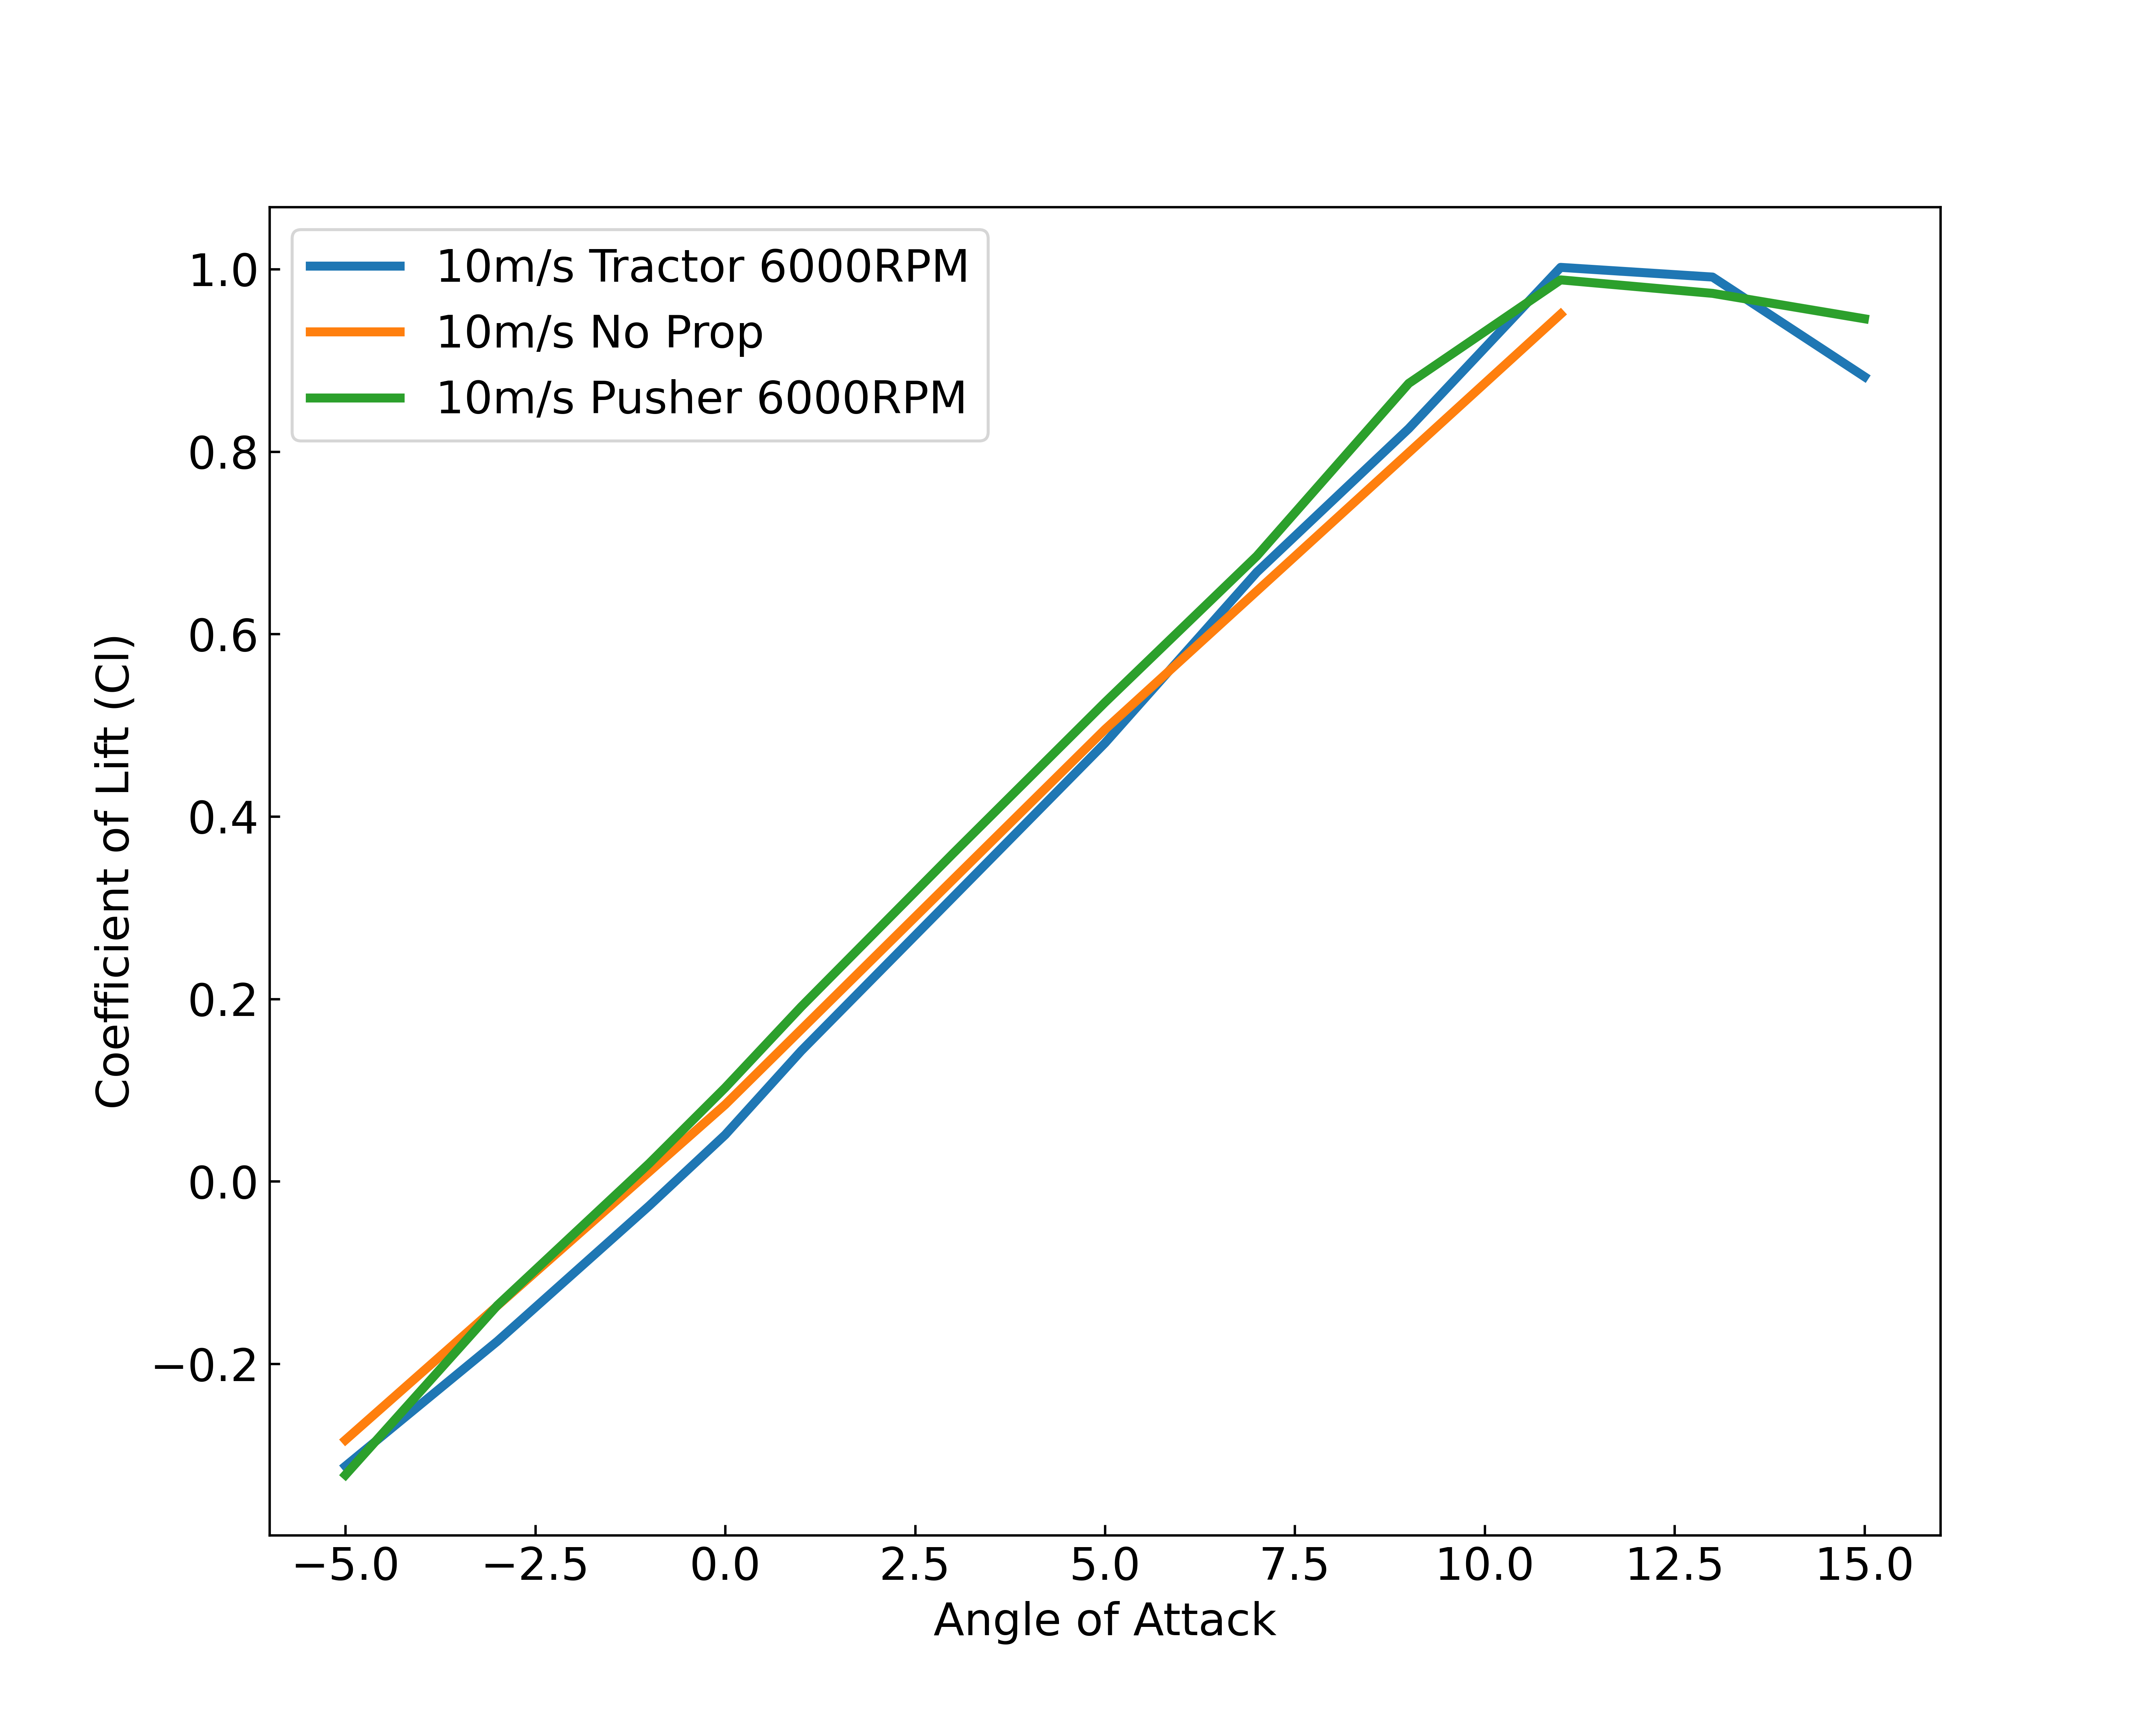
\includegraphics[width=\textwidth]{05_Results/Figs/Cl/10ms_6000RPM_Cl.png}
        \caption{Coefficient of lift at 10m/s airspeed and 6000RPM motor speed}
        \label{fig:Cl_10ms_6000}
    \end{subfigure}
    \begin{subfigure}[b]{0.467\textwidth}
        \centering
        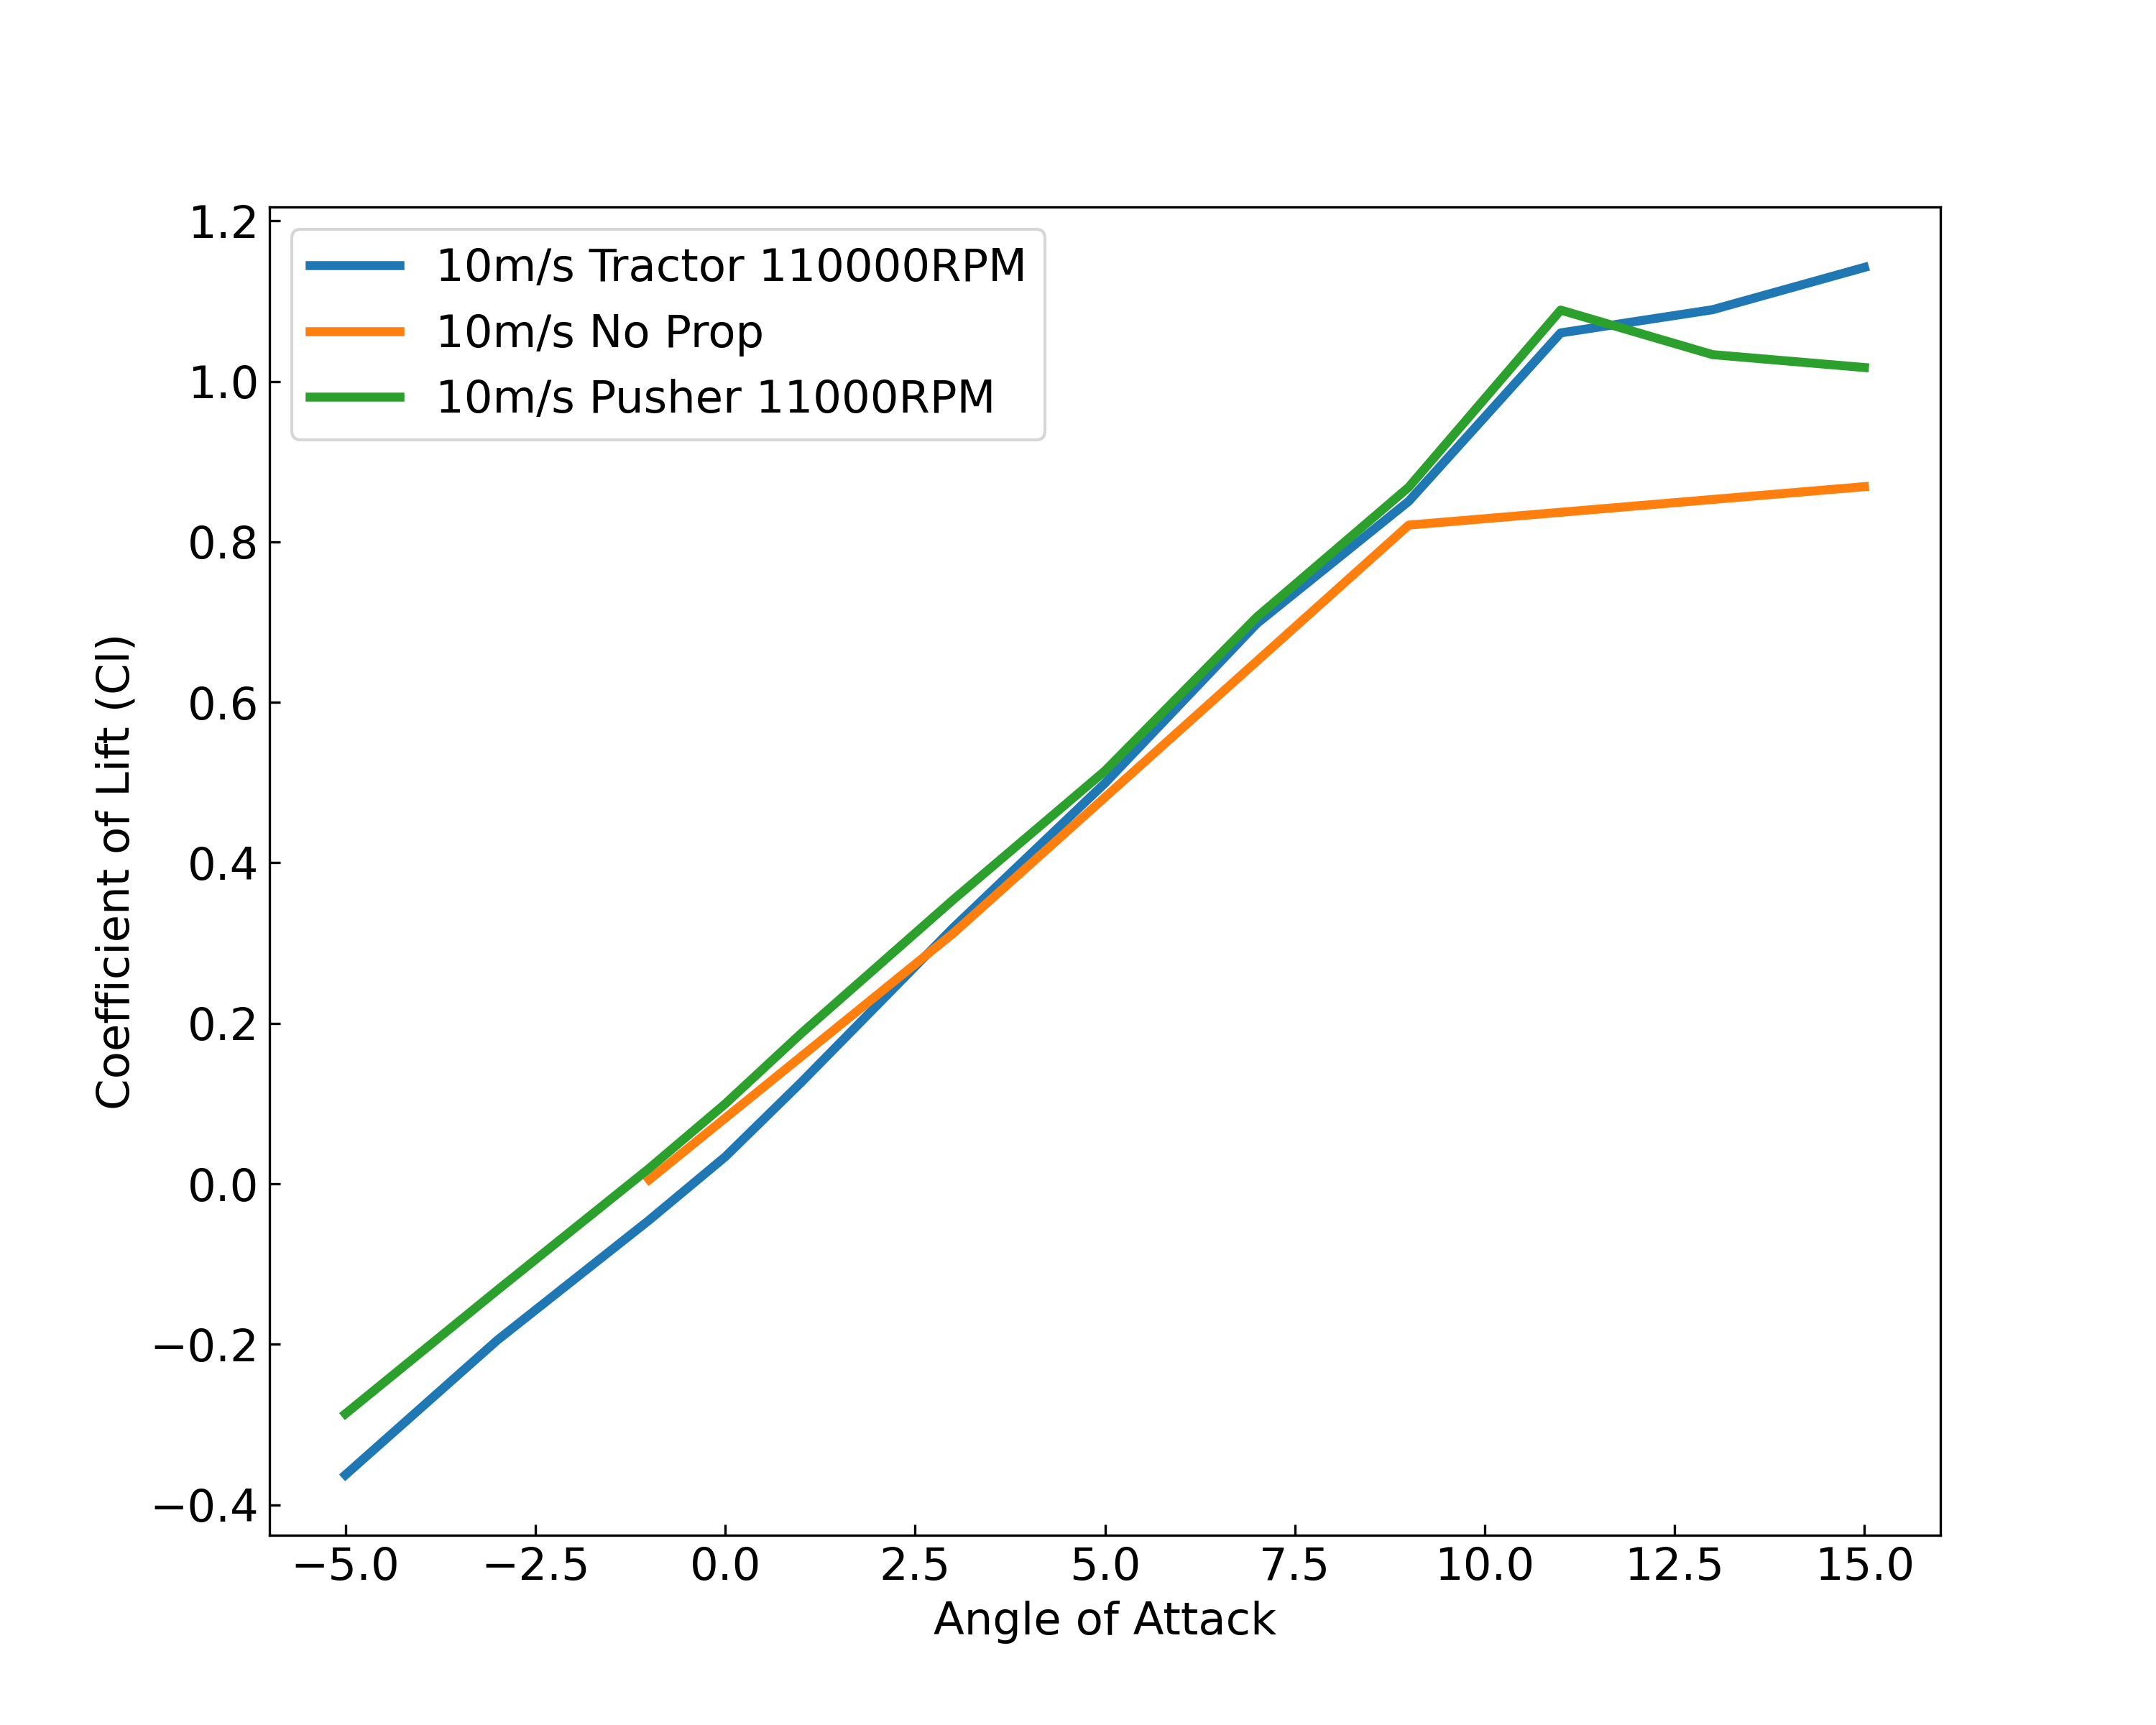
\includegraphics[width=\textwidth]{05_Results/Figs/Cl/10ms_110000RPM_Cl.png}
        \caption{Coefficient of lift at 10m/s airspeed and 11000RPM motor speed}
        \label{fig:Cl_10ms_11000}
    \end{subfigure}
    \begin{subfigure}[b]{0.467\textwidth}
        \centering
        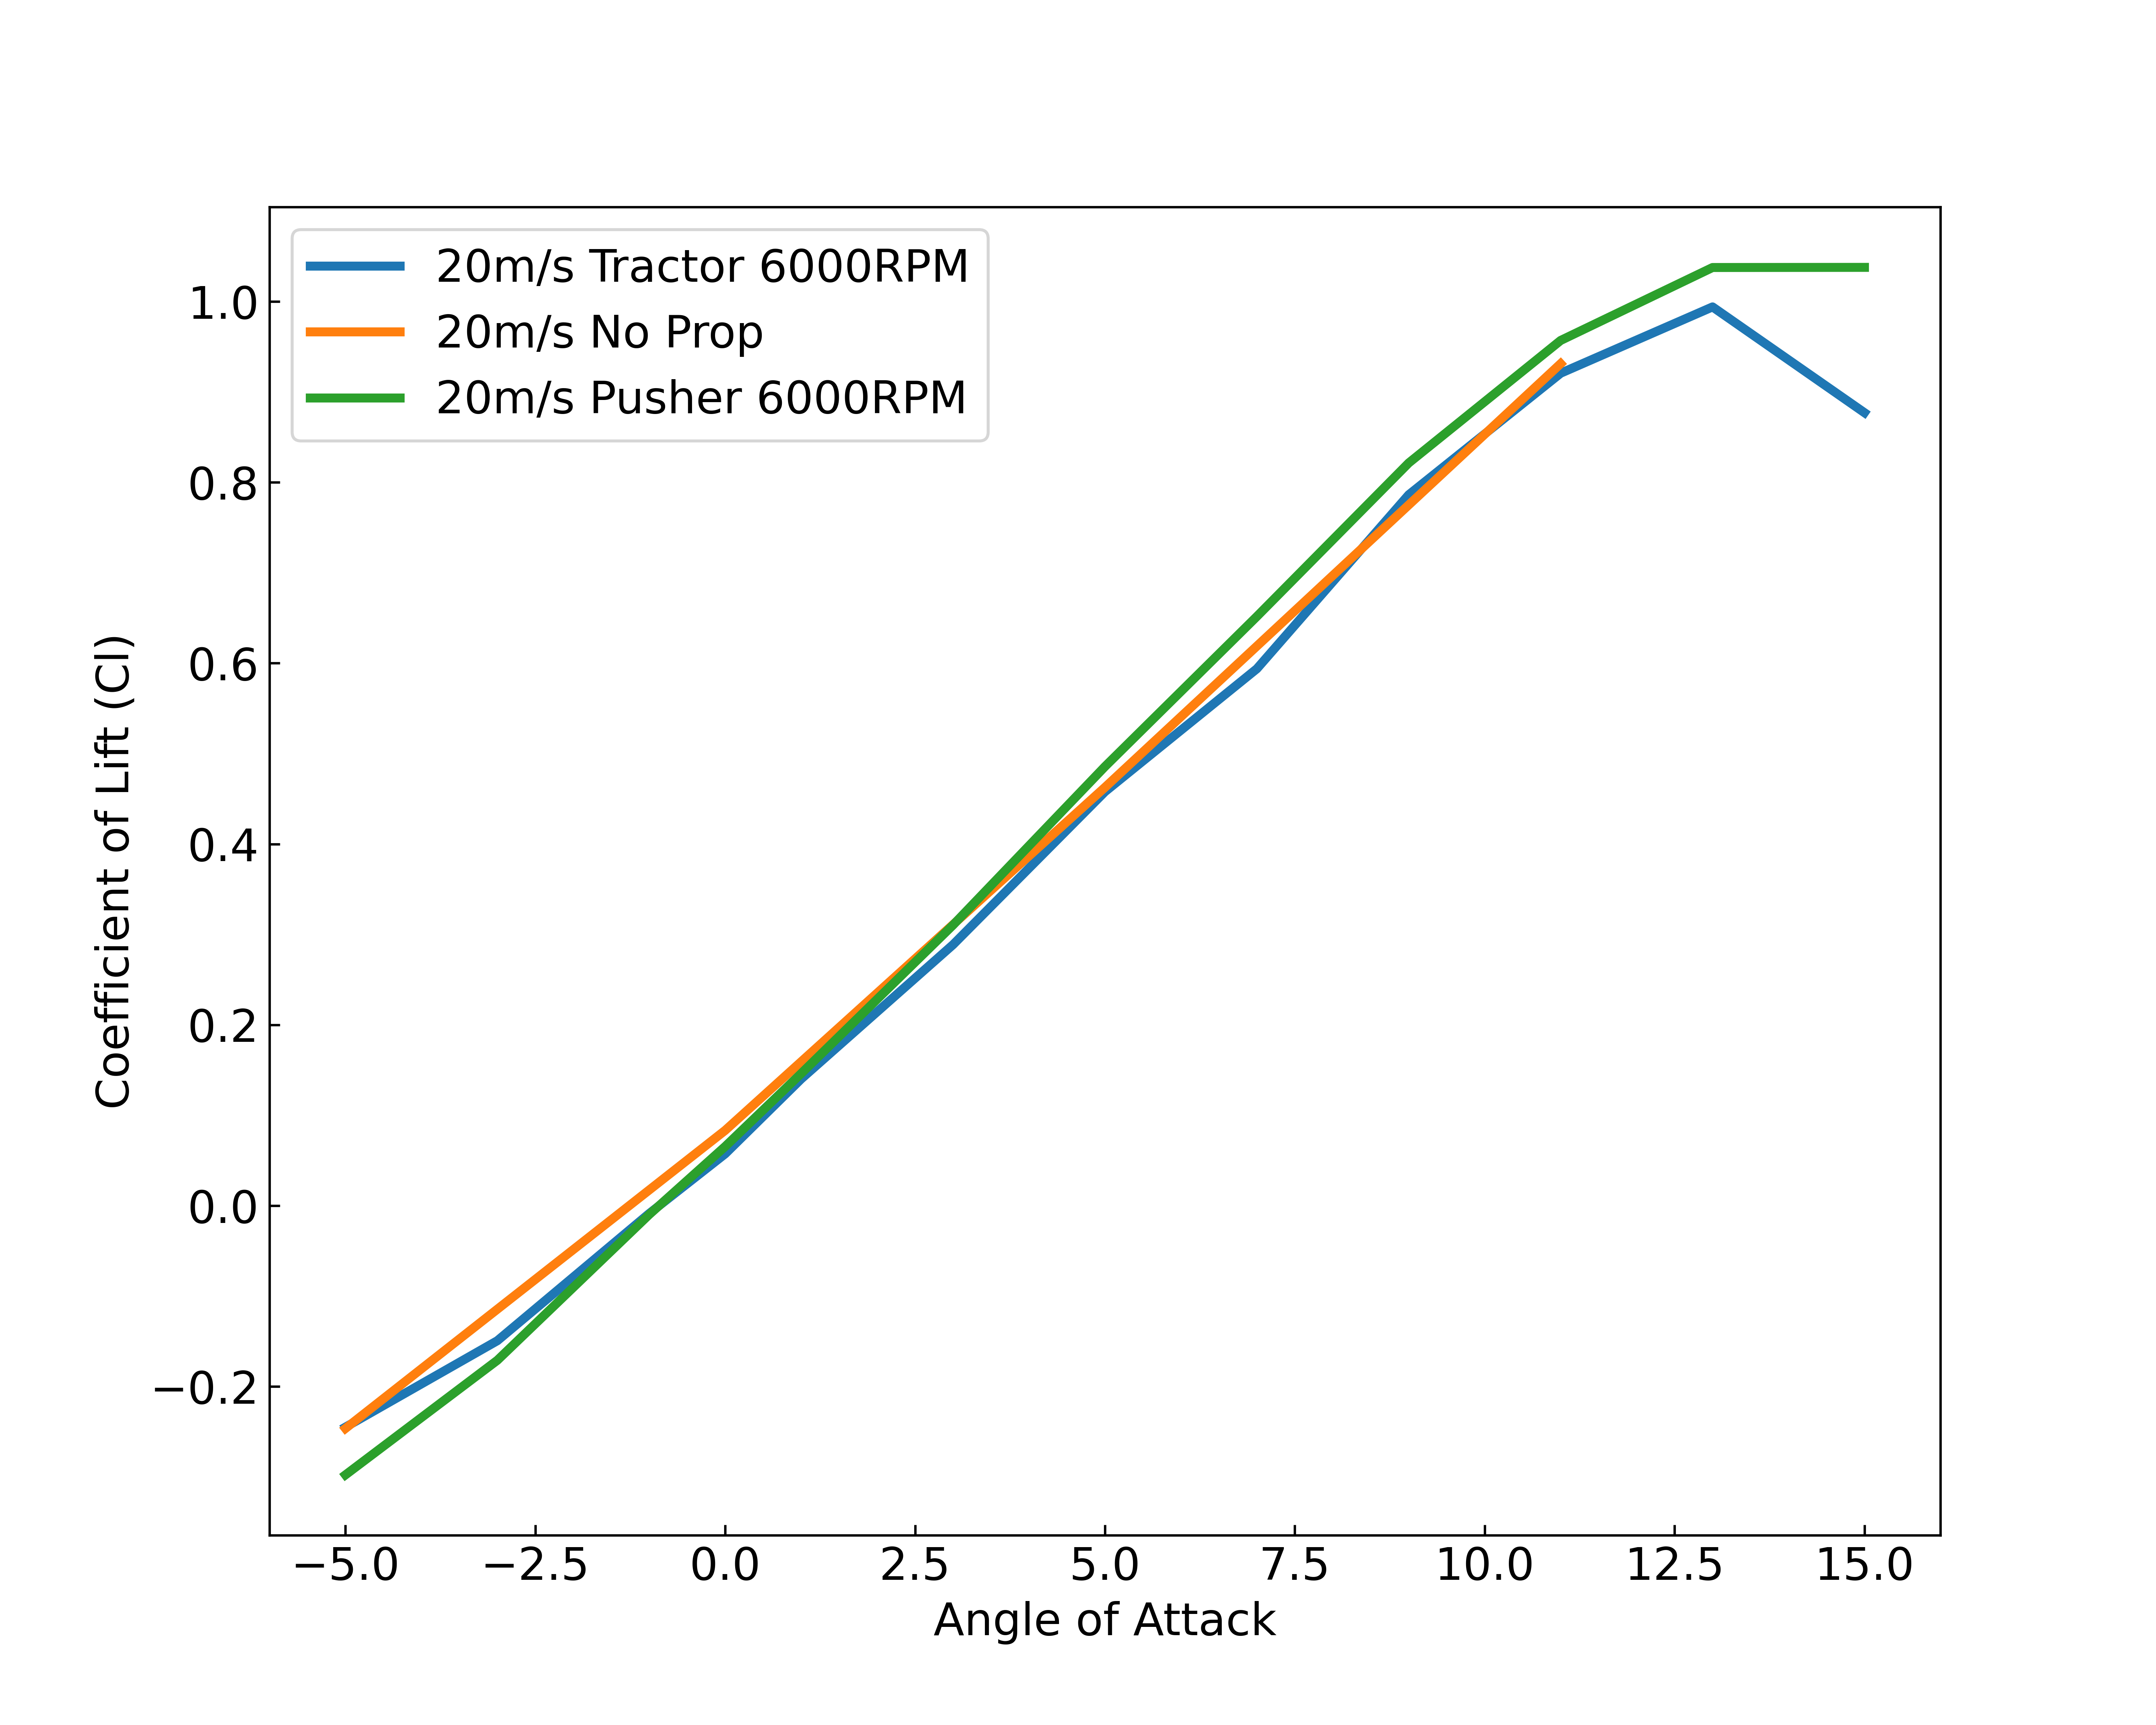
\includegraphics[width=\textwidth]{05_Results/Figs/Cl/20ms_6000RPM_Cl.png}
        \caption{Coefficient of lift at 20m/s airspeed and 6000RPM motor speed}
        \label{fig:Cl_20ms_6000}
    \end{subfigure}
    \begin{subfigure}[b]{0.467\textwidth}
        \centering
        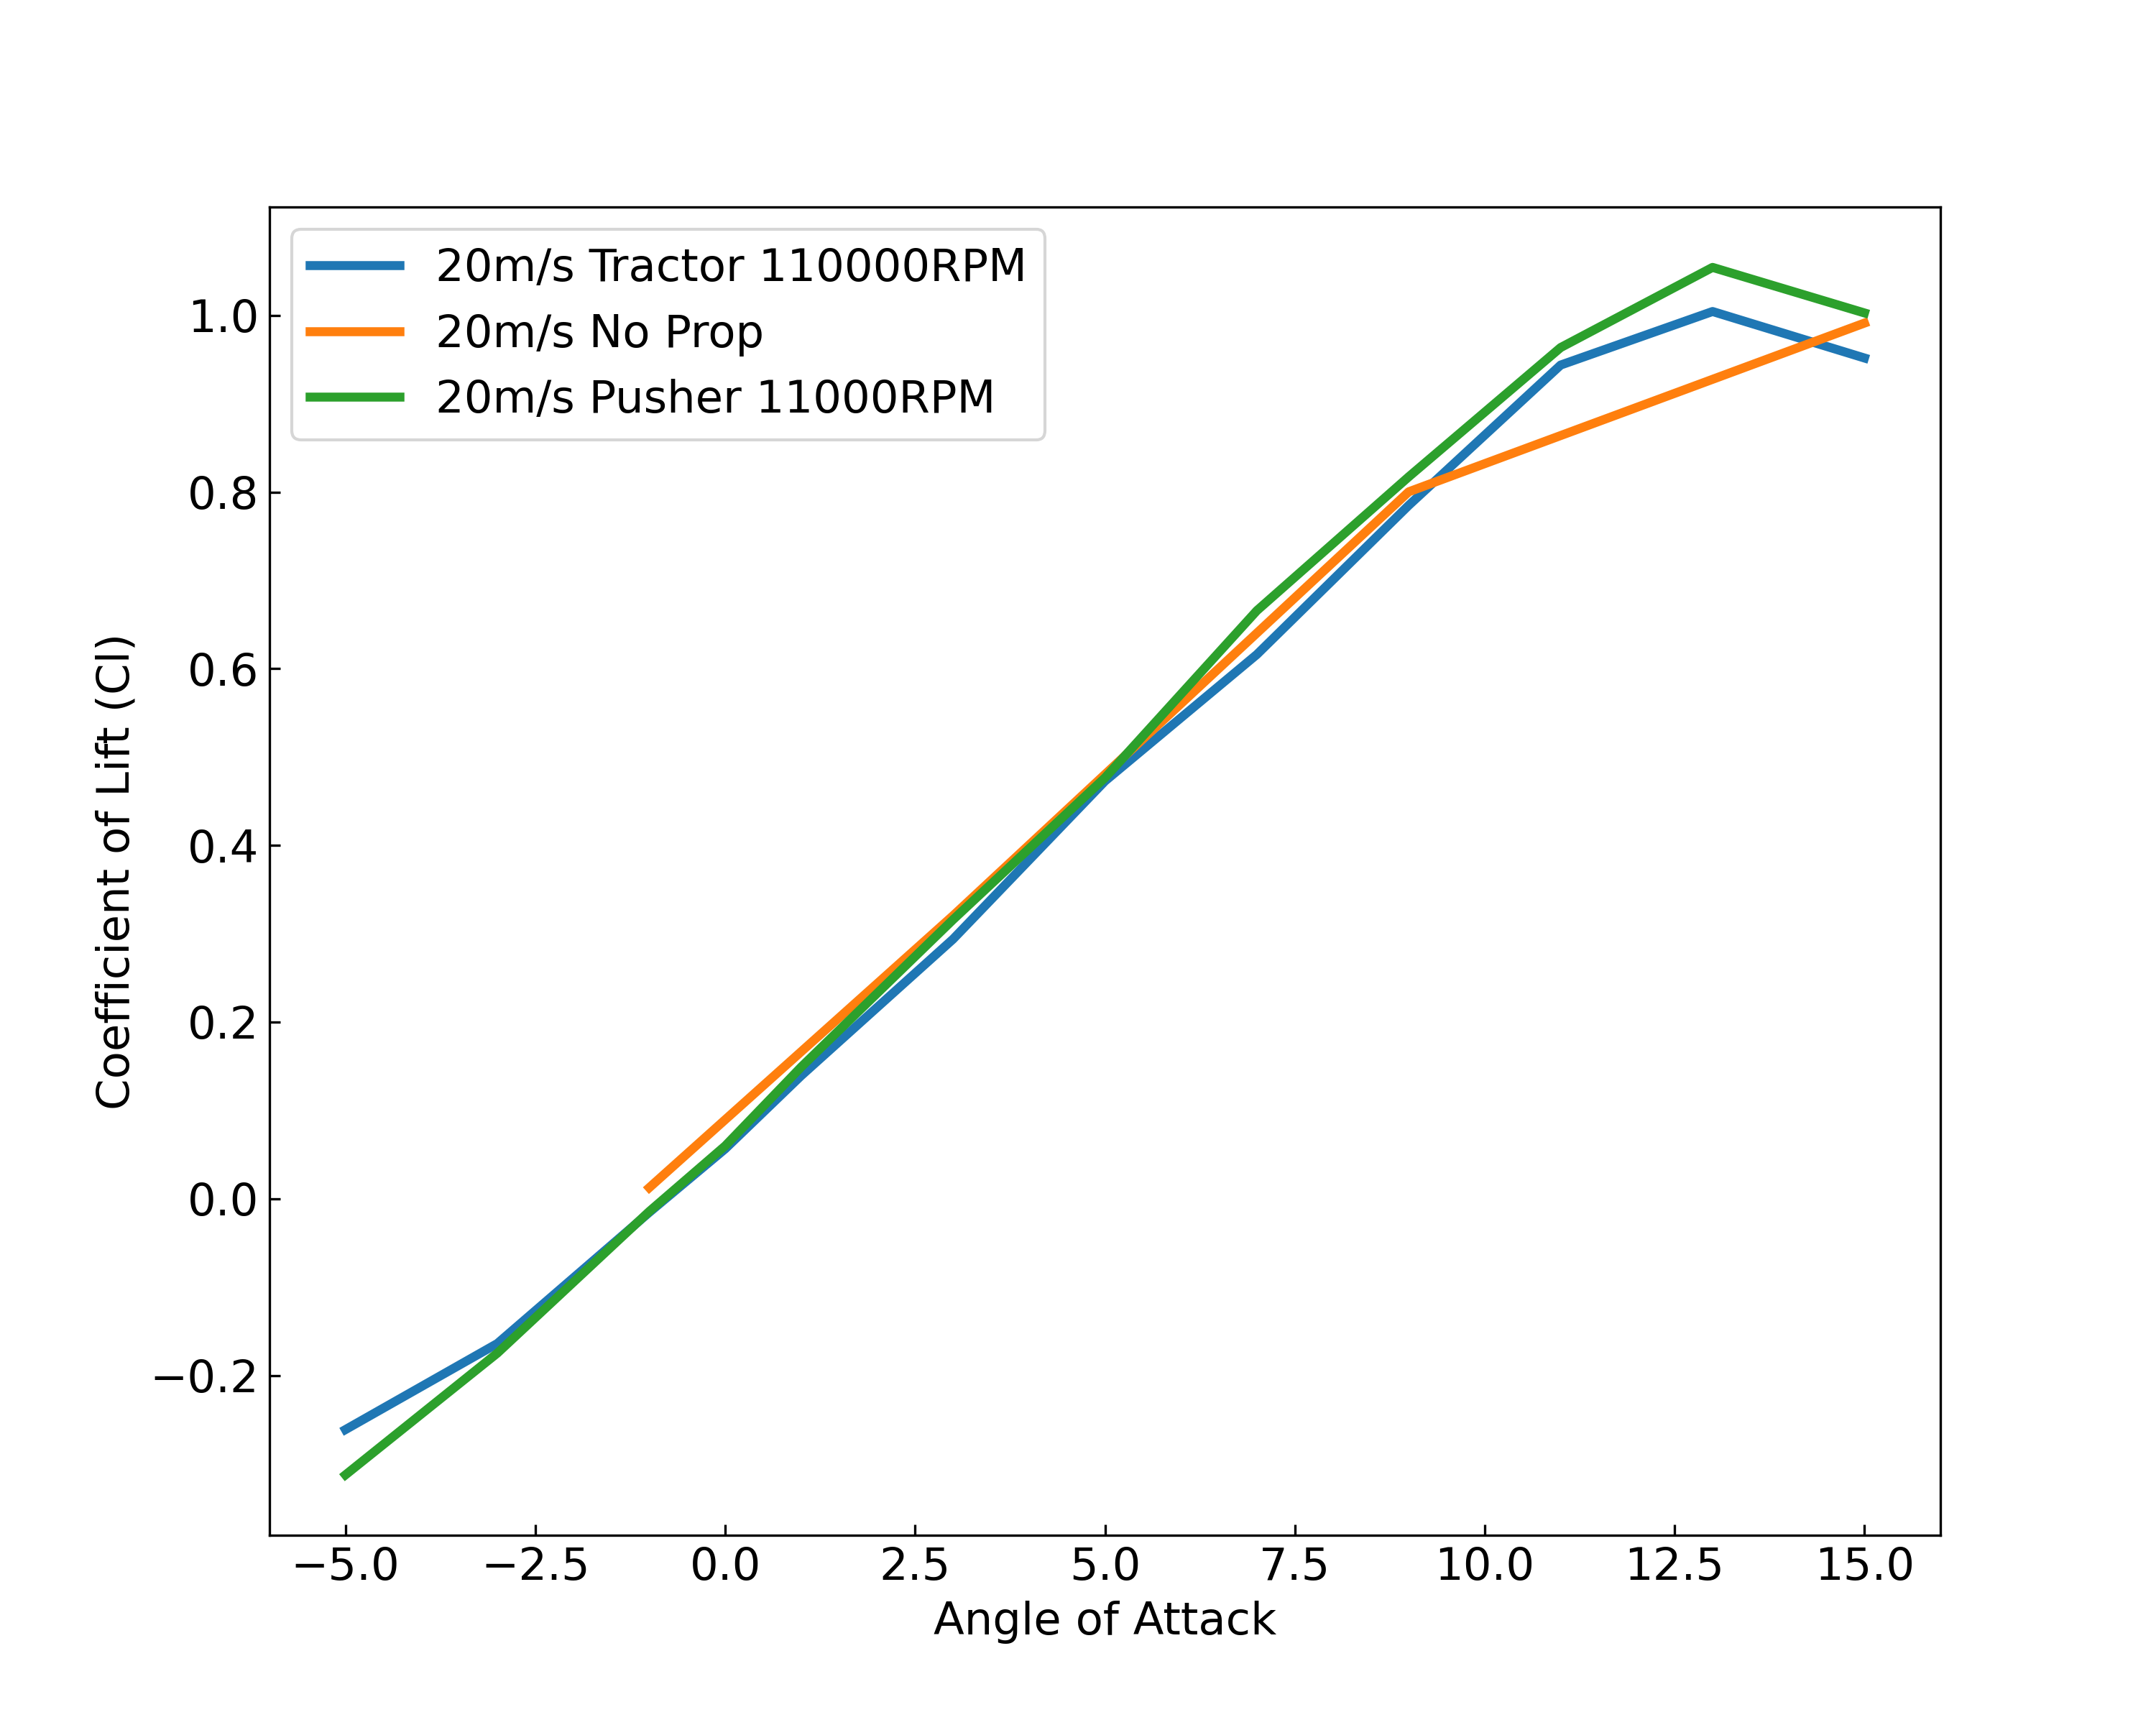
\includegraphics[width=\textwidth]{05_Results/Figs/Cl/20ms_110000RPM_Cl.png}
        \caption{Coefficient of lift at 20m/s airspeed and 11000RPM motor speed}
        \label{fig:Cl_20ms_11000}
    \end{subfigure}
    \caption{Coefficient of lift variation with various conditions for the pusher, tractor and no propeller configurations }
\end{figure}

\subsection{Aerodynamic Coefficient of Drag}
Figure \ref{fig:Cd_11000RPM} shows that as the airspeed of the wind tunnel increased the coefficient of drag shifted upwards for both the pusher and tractor configration. The drag for both the tractor and puller configuration at 10m$s^{-1}$ airspeed is negative an indicates that the drag on the MAV model is being reduced with the addition of the propeller to the MAV model. The highest coefficient of drag is seen when no propeller is operating on the MAV model. When no propeller is added, no significant changes are seen with airspeed for the coefficient of drag. The tractor configuration in general reduces drag compared with the pusher configuration, this is most clearly seen at 20m$s^{-1}$ in Figure \ref{fig:Cd_11000RPM}. As the airspeed increases the coefficient of drag is also seen to increase for the pusher and tractor configuration.
\todo{change line style here }
begin{figure}[H]
    \centering
    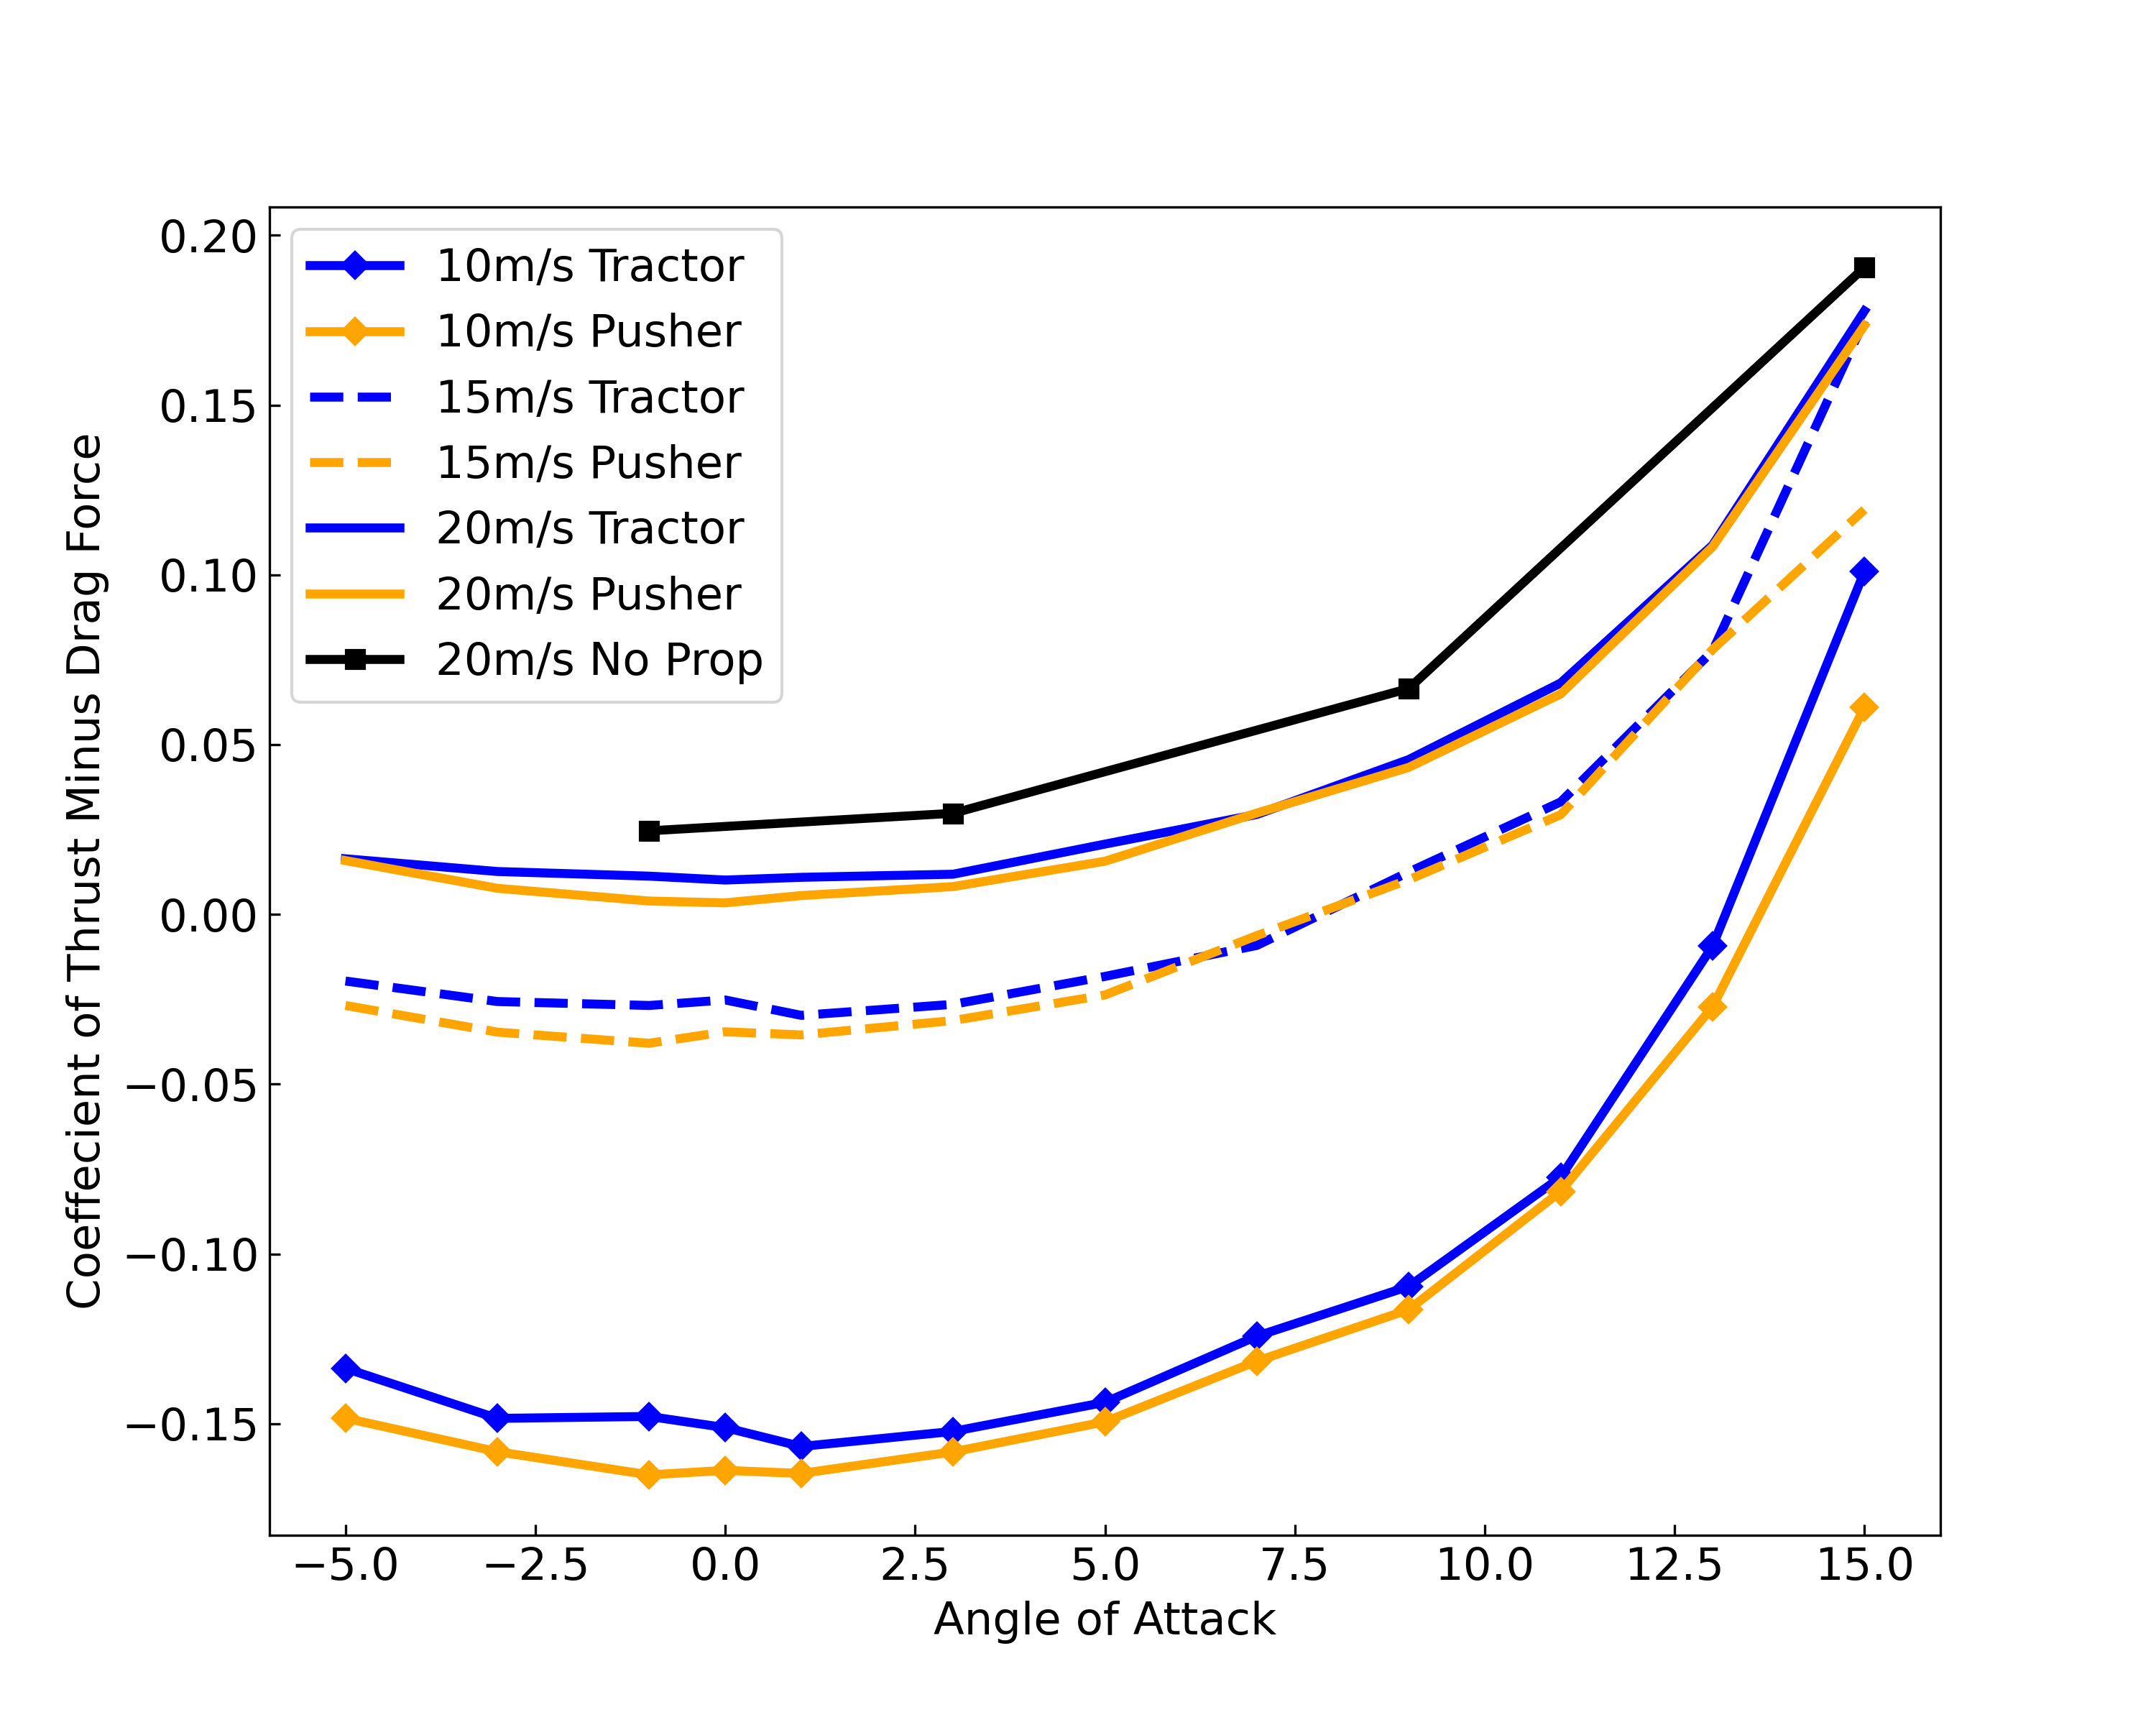
\includegraphics[scale = 0.7]{05_Results/Figs/Cd/110000RPM_Cd.png}
    \caption{Coefficient of drag variation at 11000RPM motor speed for the tractor, pusher and no propeller configurations}
    \label{fig:Cd_11000RPM}
\end{figure}
Figure \ref{fig:Cd_20ms} shows minimal differences between the pusher and tractor configurations. The addition of the propeller increases drag at 6000RPM, however as the motor speed increases to 11000RPM there is a significant drop in the coefficient of drag for both the tractor and pusher configuration. 
\todo{get rid of extra no prop lines - keep one only}
\begin{figure}[H]
    \centering
    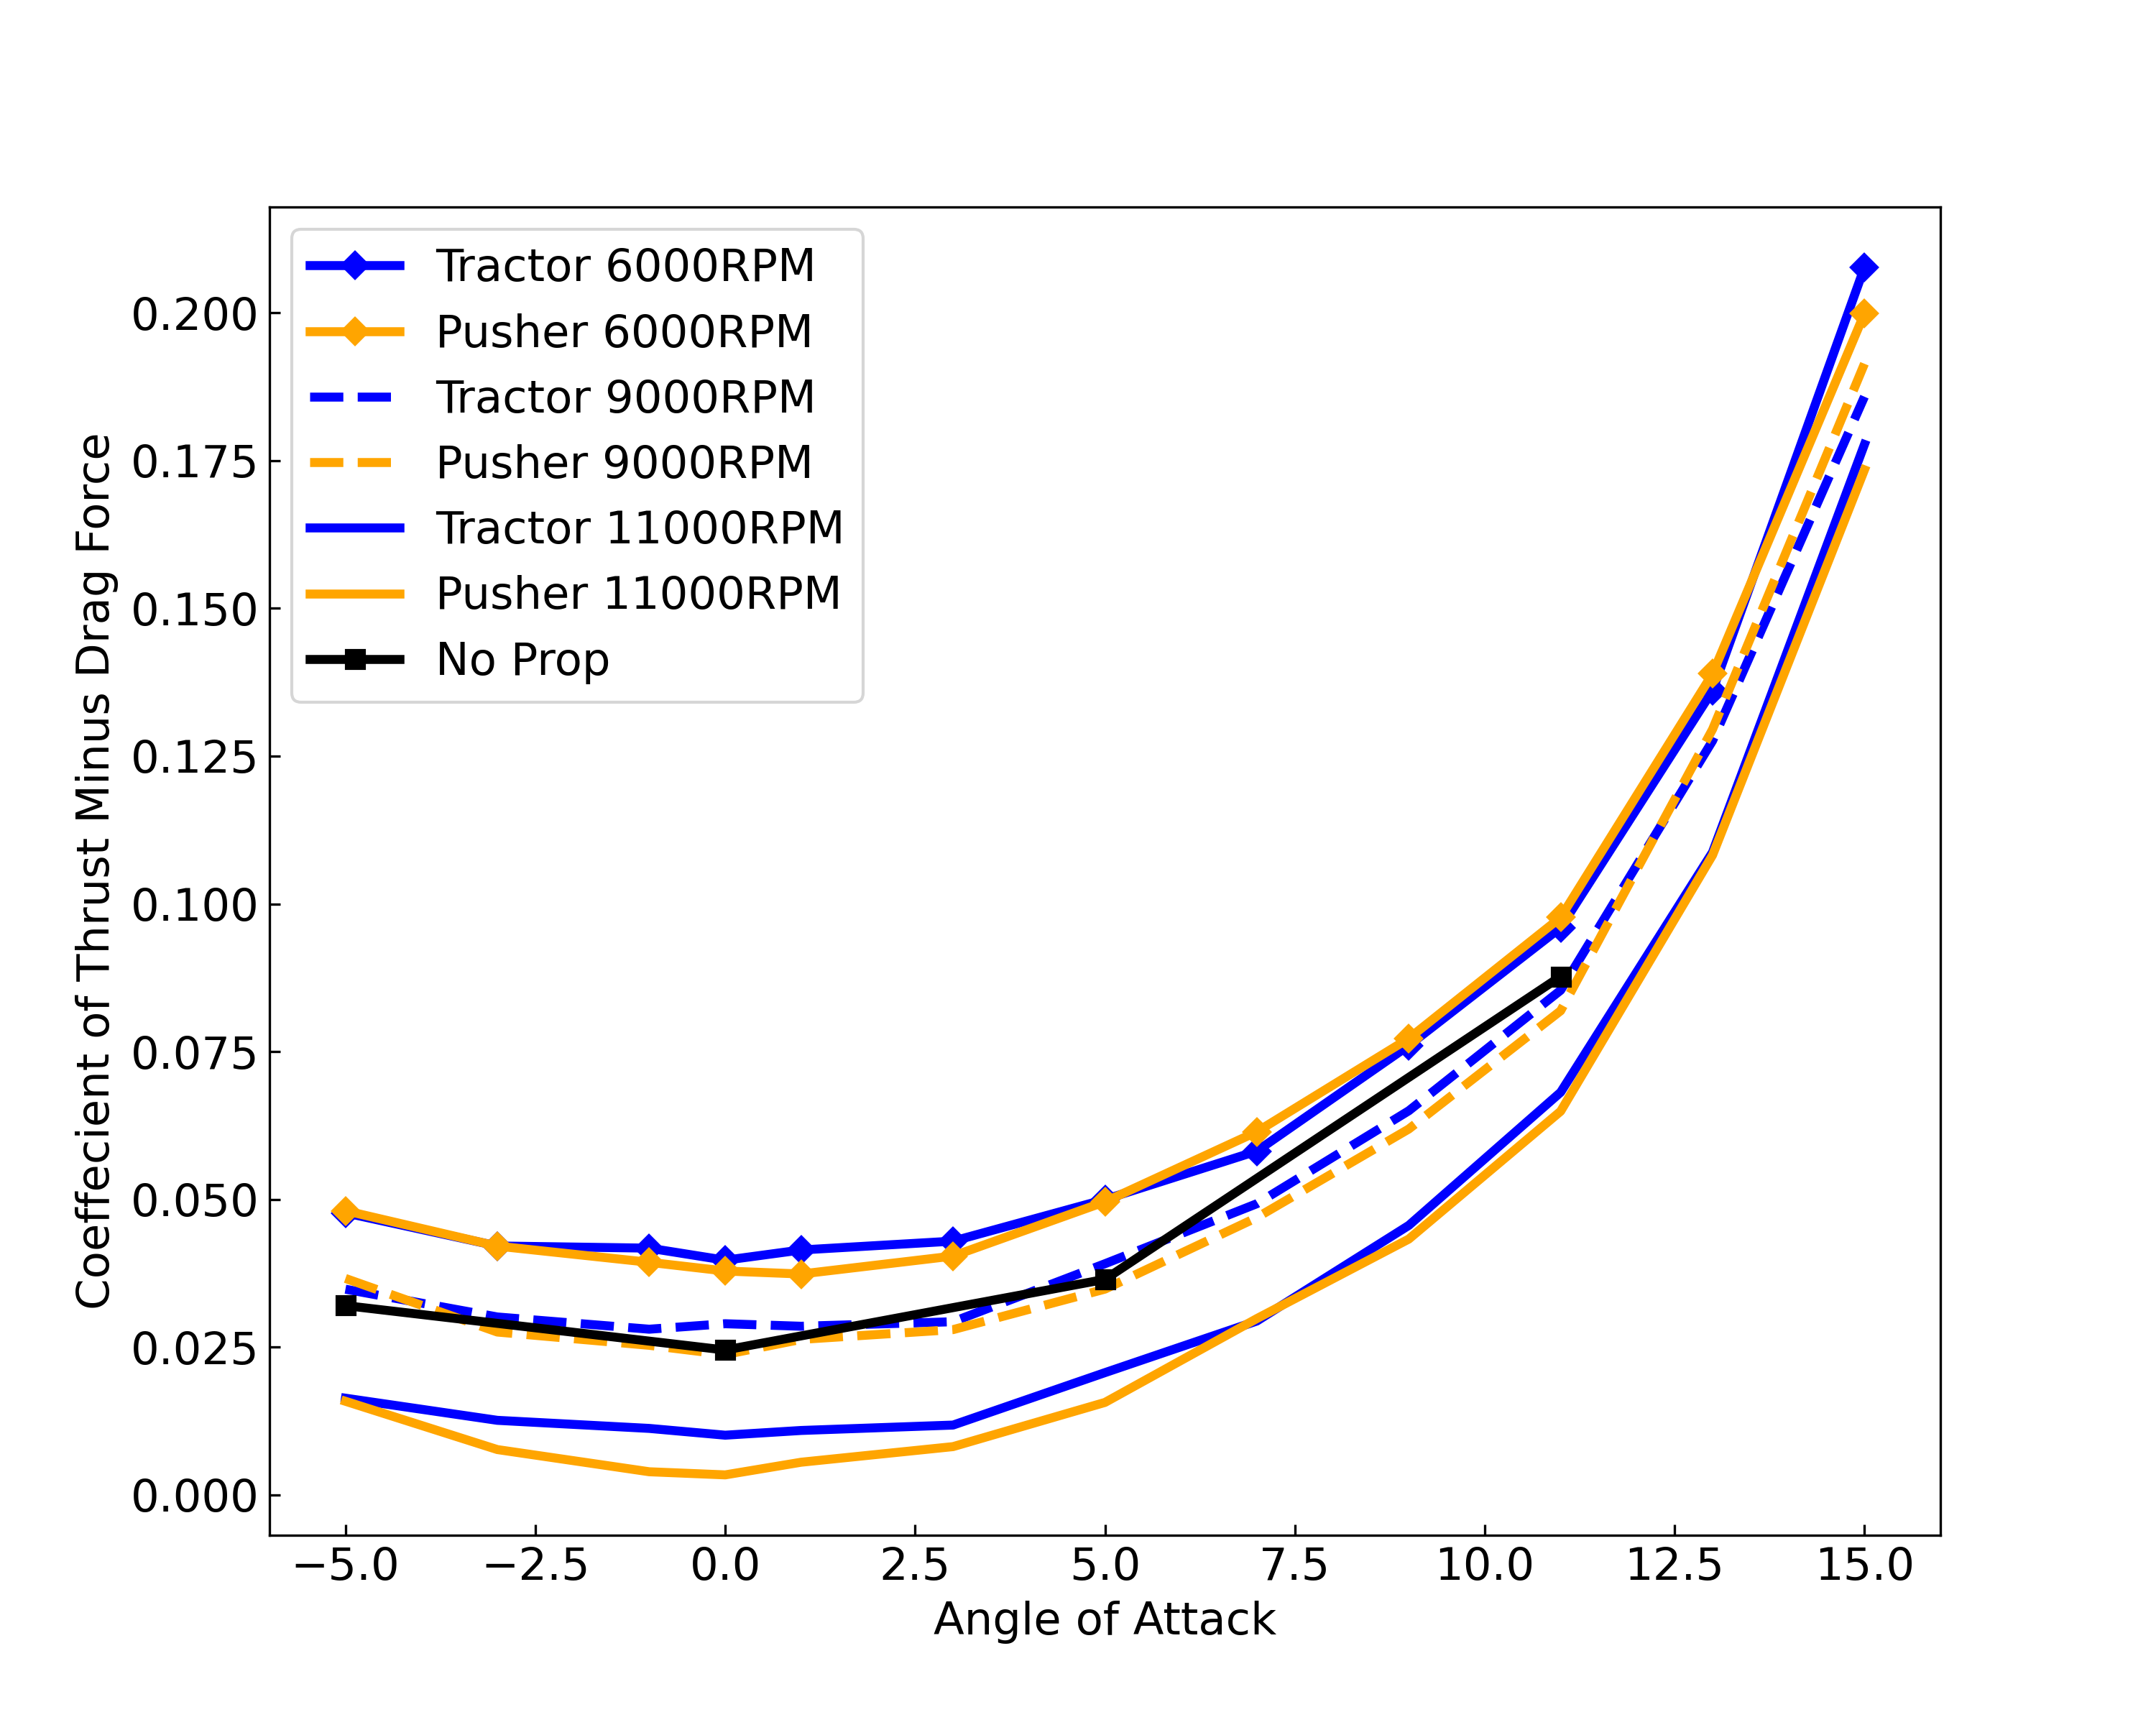
\includegraphics[scale = 0.7]{05_Results/Figs/Cd/20ms_Cd.png}
    \caption{Coefficient of drag variation at 20ms airspeed for the tractor, pusher and no propeller configuration}
    \label{fig:Cd_20ms}
\end{figure}

\subsection{Pitching Moment Coefficient}

Figure \ref{fig:Cm_graphs} shows that as the motor speed increases from 6000RPM to 11000RPM the tractor configuration experienced a decrease in pitching coefficient compared with the no propeller model up until stall at approximately 12$^\circ$ angle of attack. The pusher configration experienced an increase in the pitching moment compared with the no propeller model. Increasing the airspeed decreased the pitching moment for all motor speeds.

\begin{figure}[H]
    \centering
    \begin{subfigure}[b]{0.467\textwidth}
        \centering
        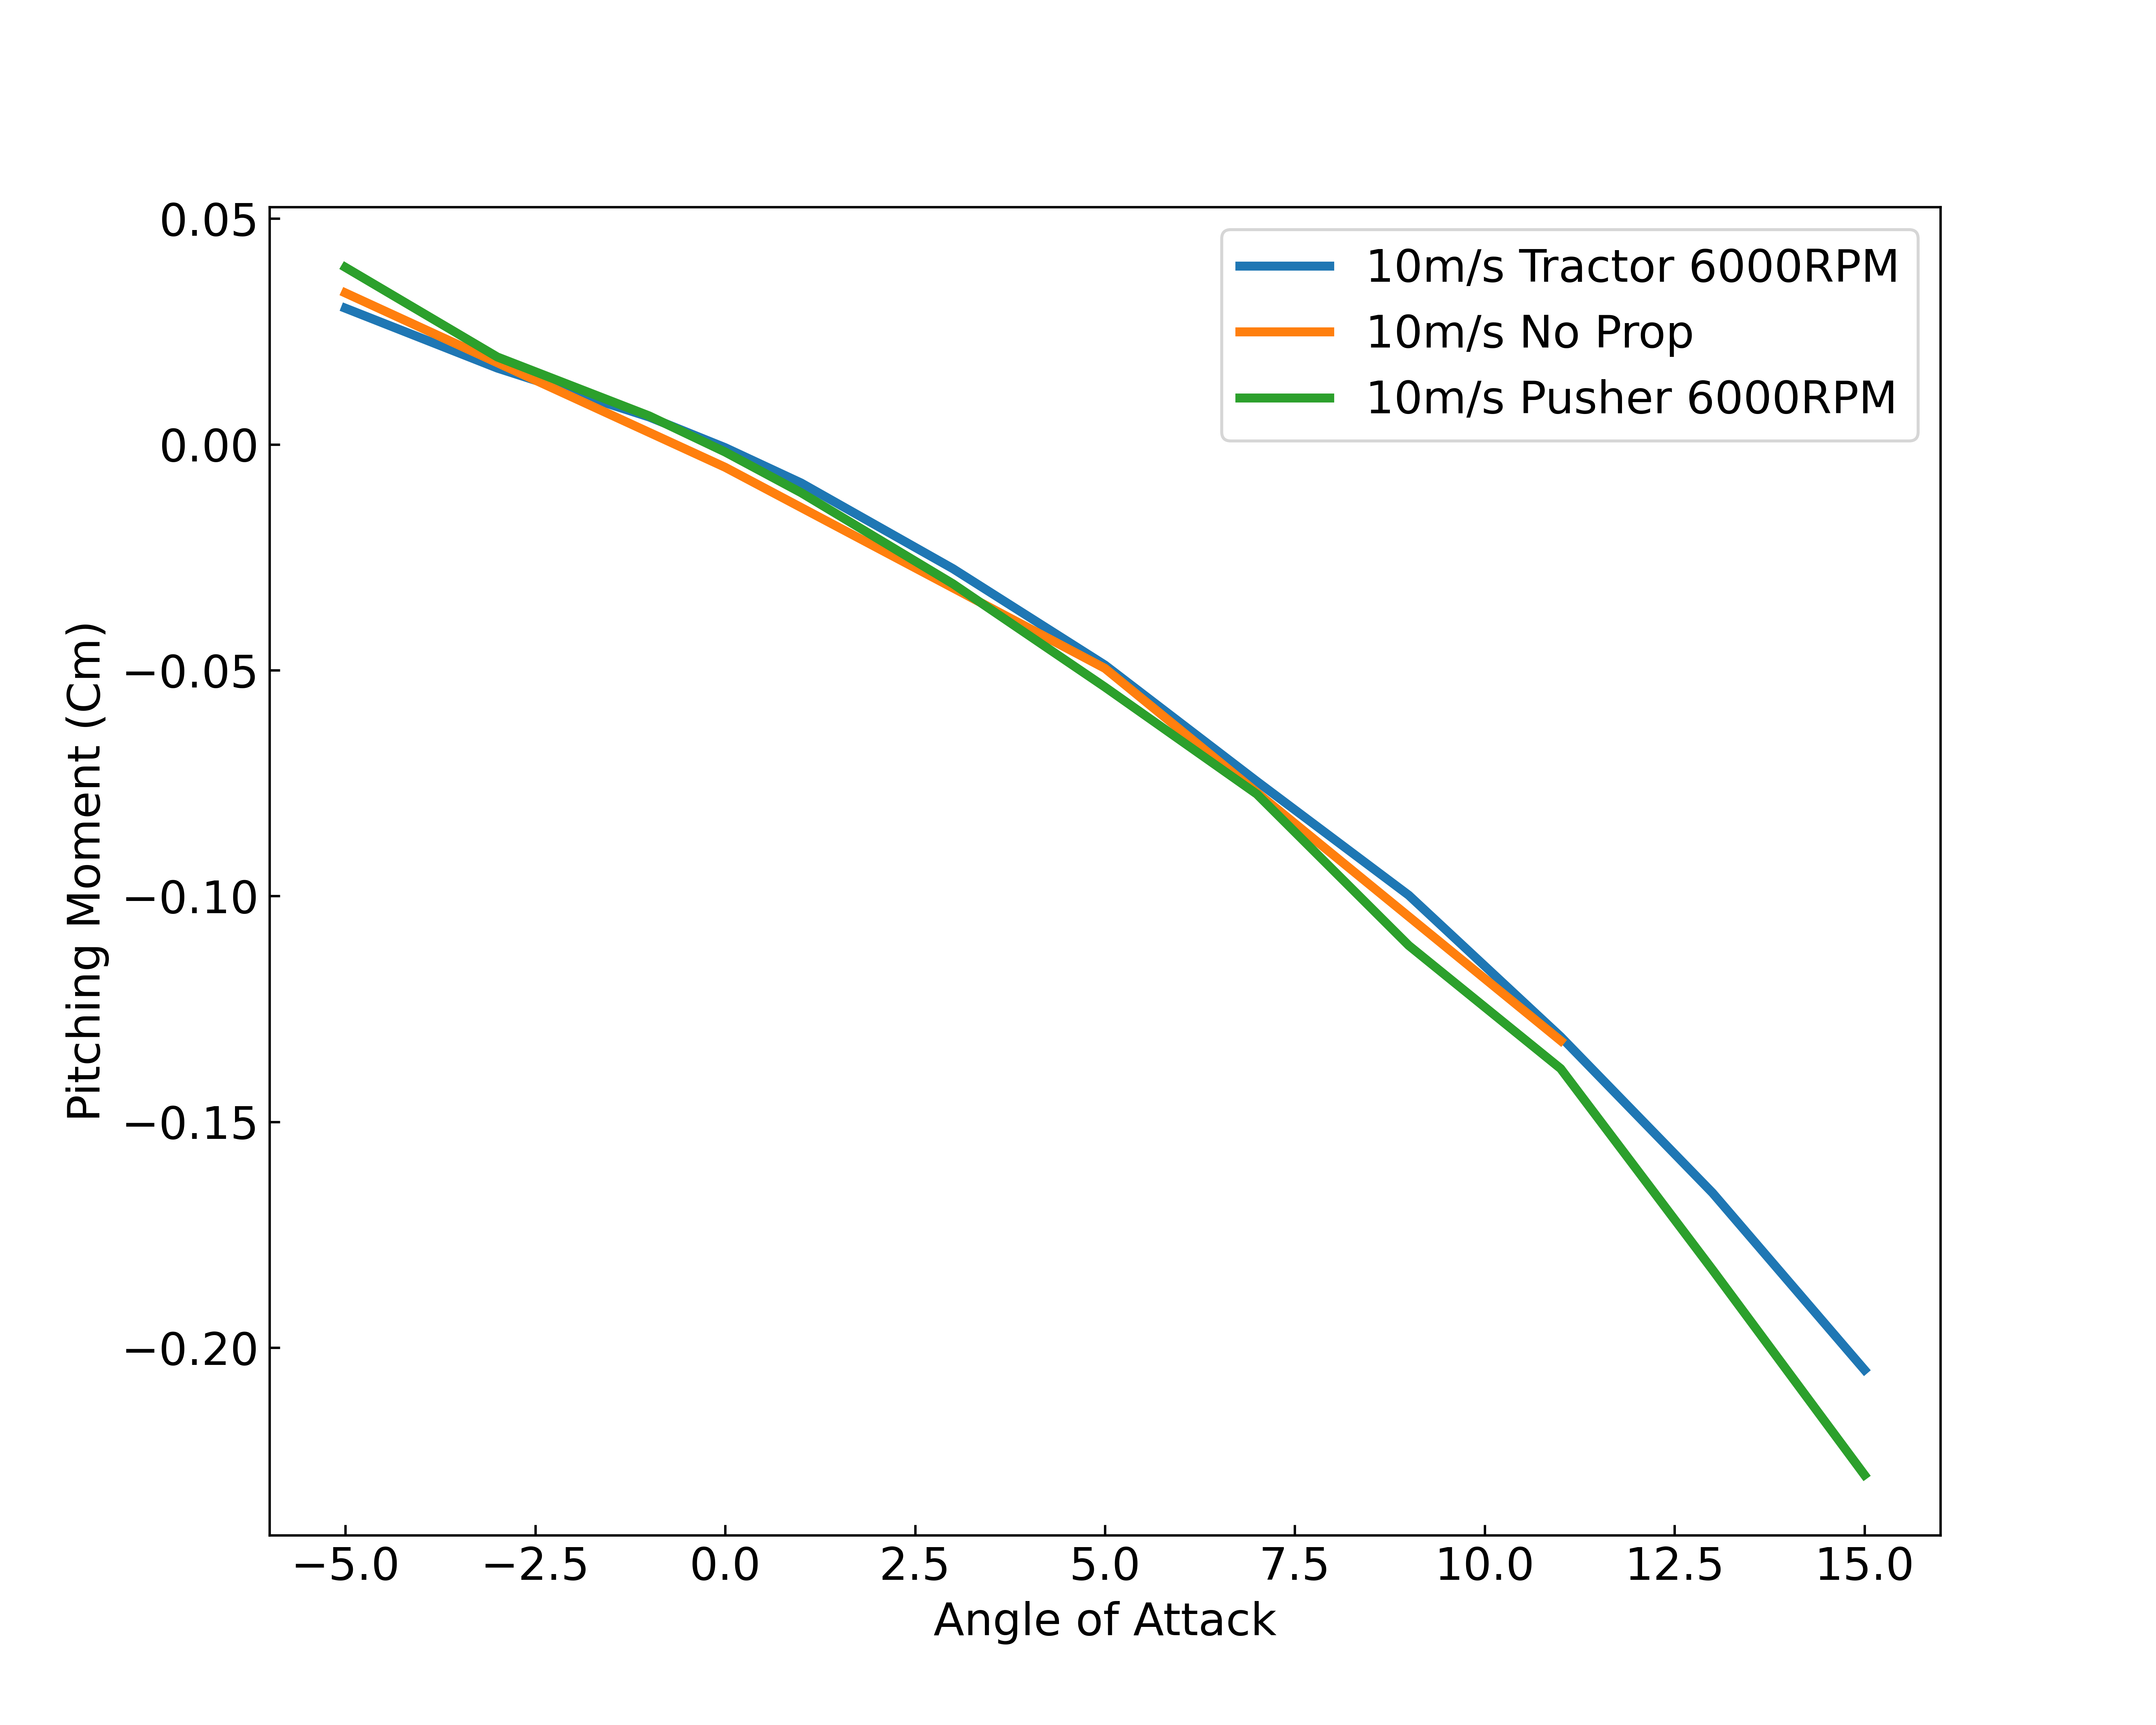
\includegraphics[width=\textwidth]{05_Results/Figs/Cm/10ms_6000RPM_Cm.png}
        \caption{Pitching Moment Coefficient at 10m/s airspeed and 6000RPM motor speed}
        \label{fig:Cm_10ms_6000}
    \end{subfigure}
    \begin{subfigure}[b]{0.467\textwidth}
        \centering
        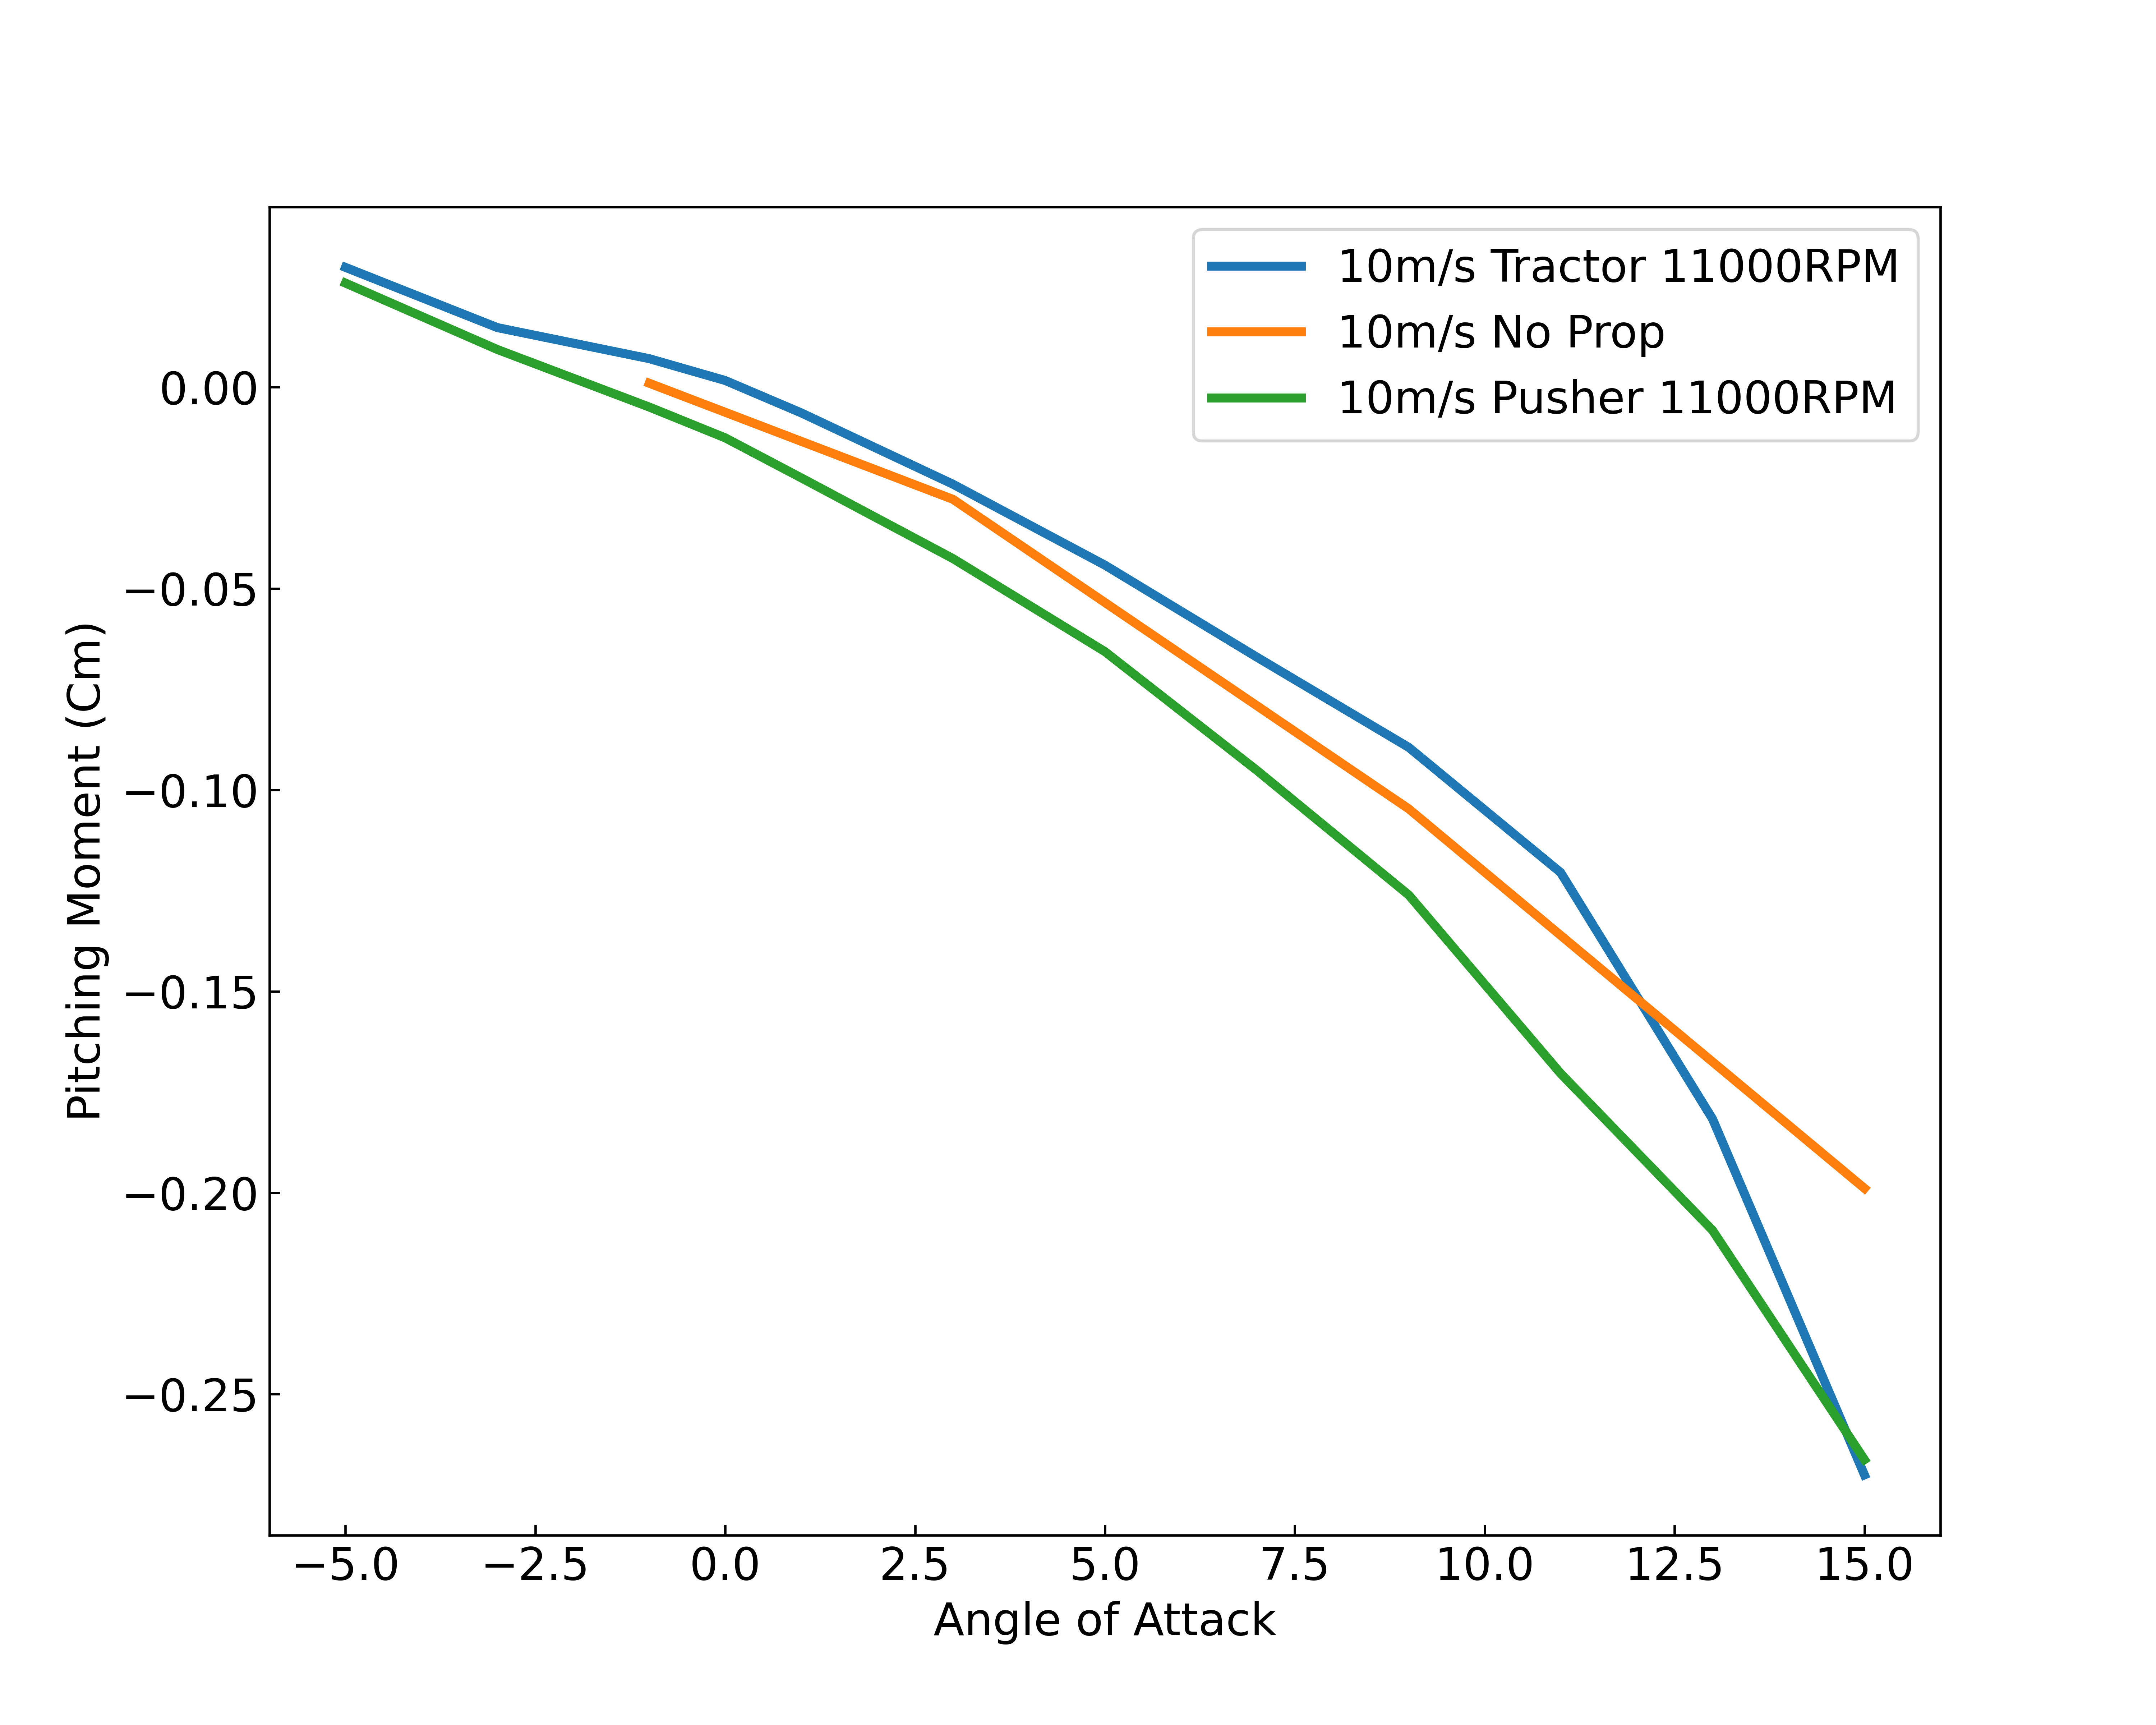
\includegraphics[width=\textwidth]{05_Results/Figs/Cm/10ms_11000RPM_Cm.png}
        \caption{Pitching Moment Coefficient at 10m/s airspeed and 11000RPM motor speed}
        \label{fig:Cm_10ms_11000}
    \end{subfigure}
    \begin{subfigure}[b]{0.467\textwidth}
        \centering
        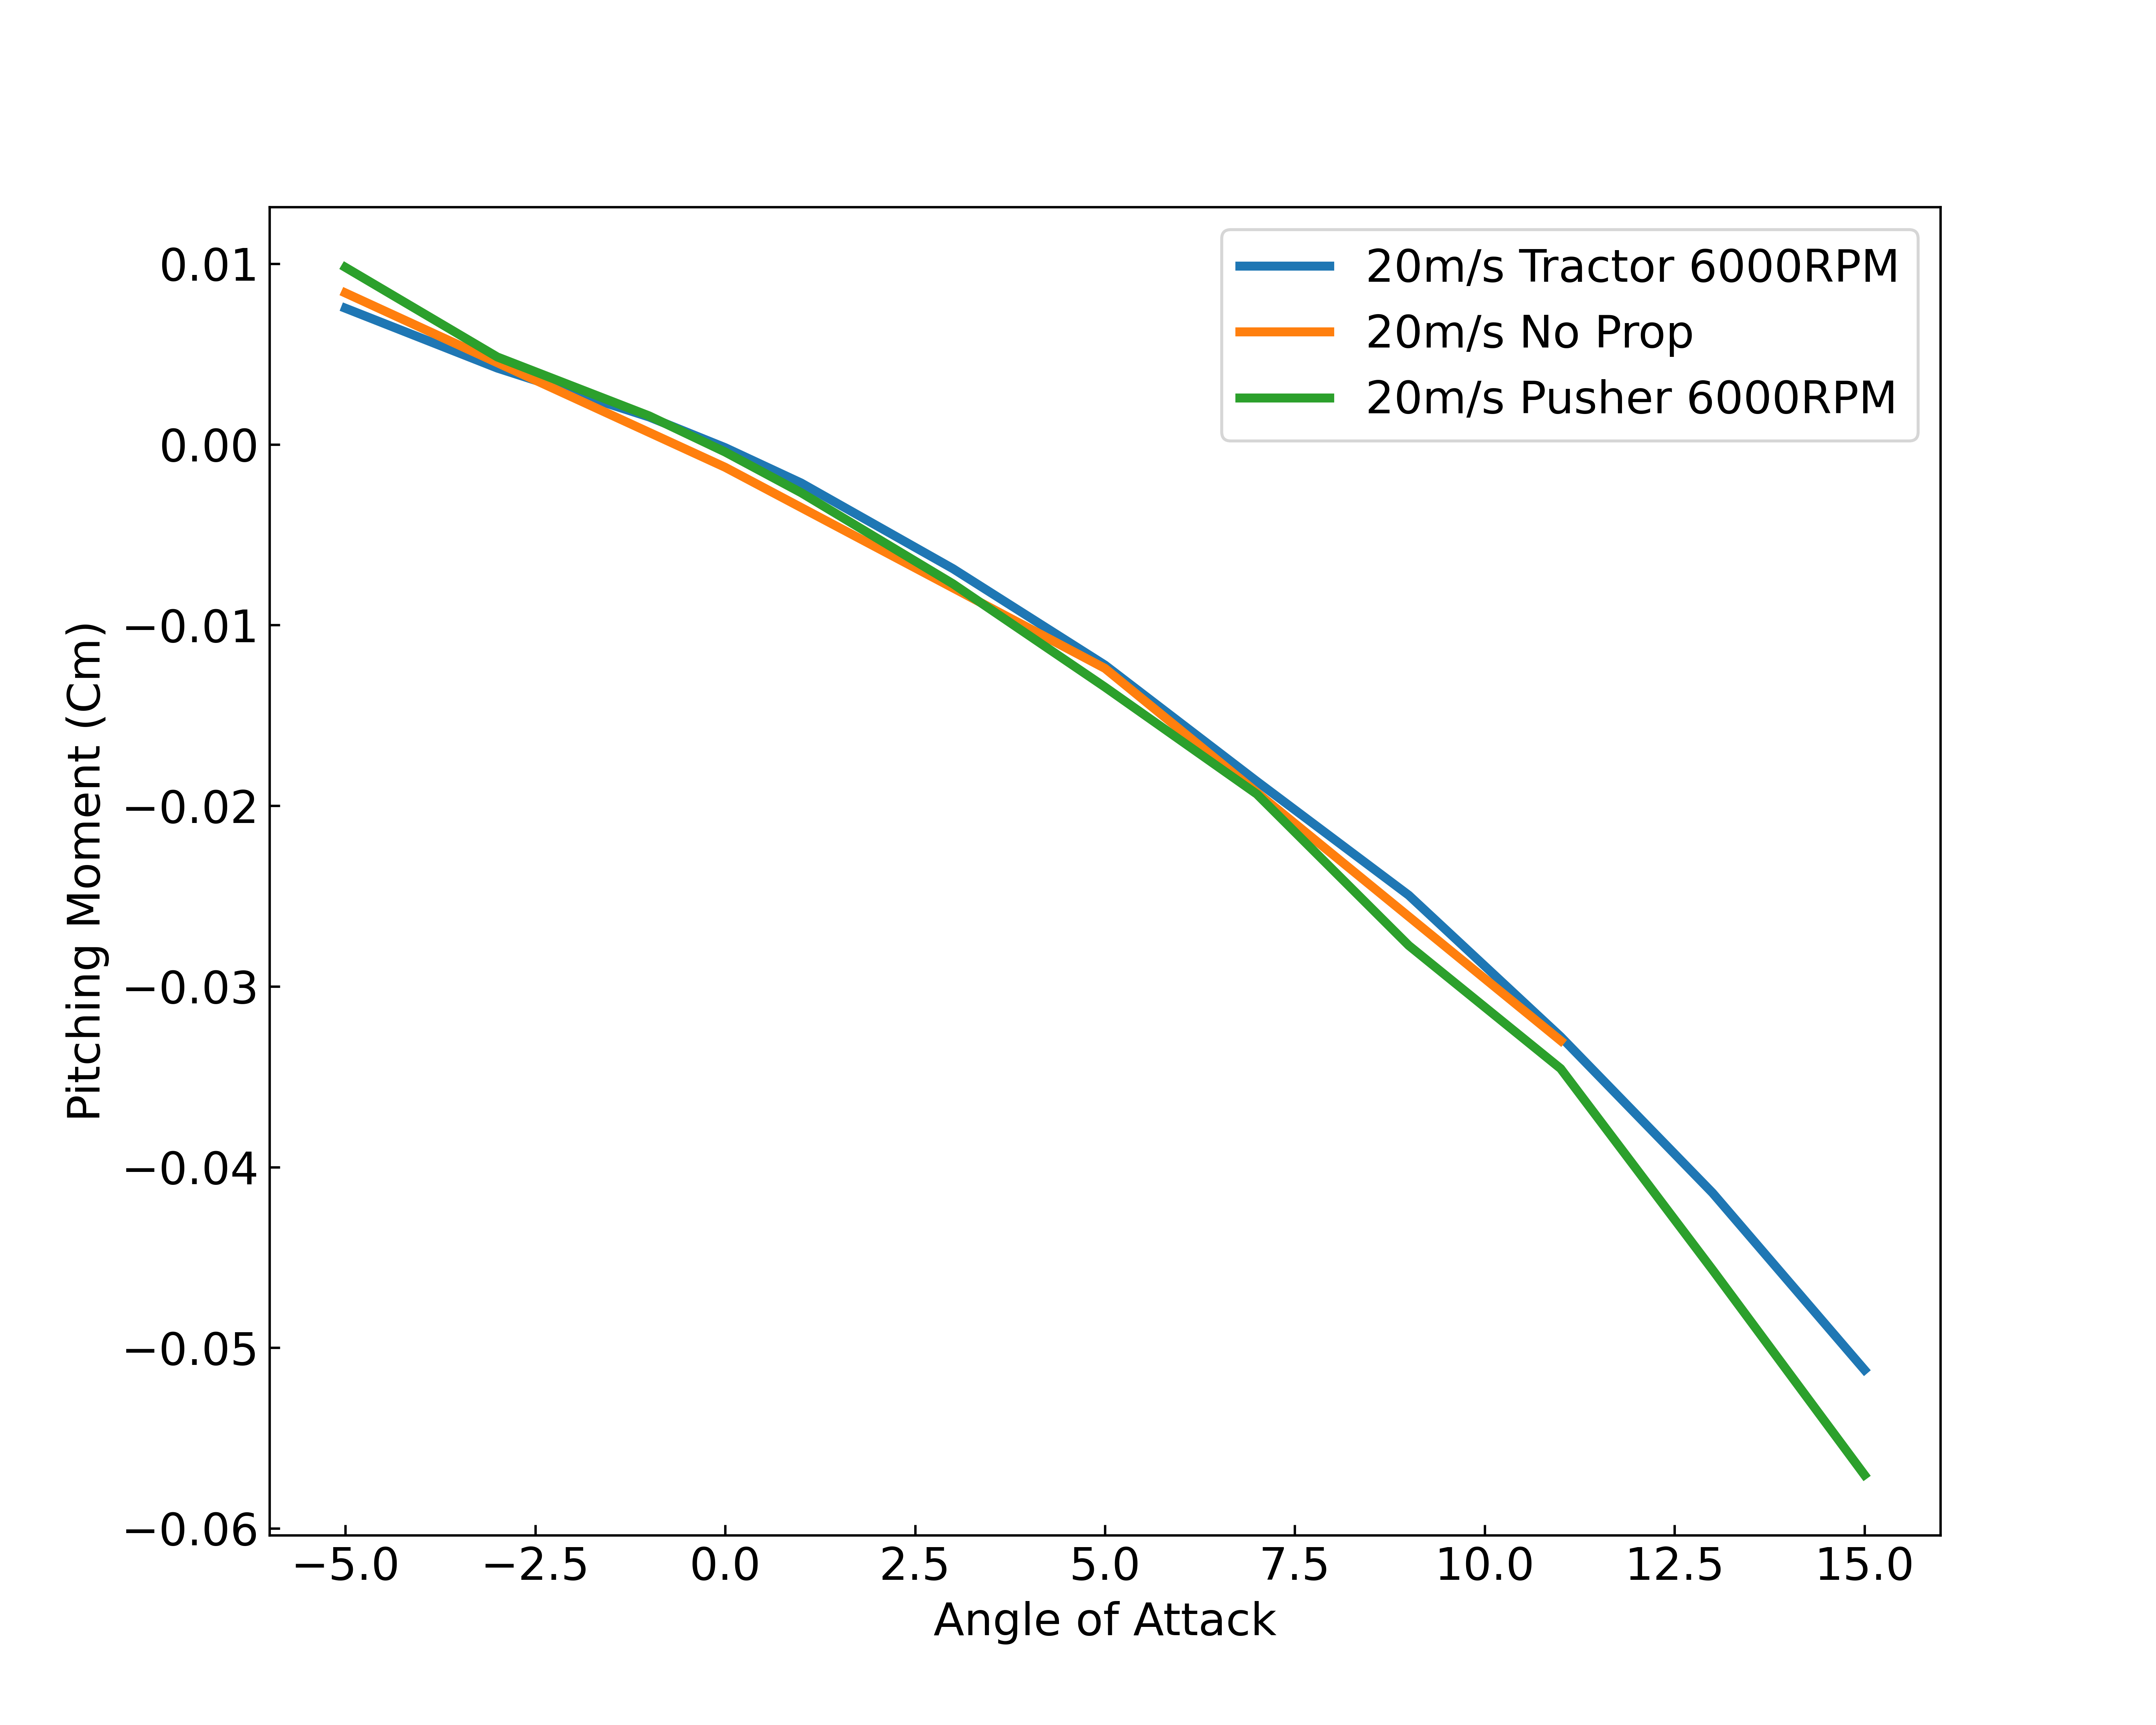
\includegraphics[width=\textwidth]{05_Results/Figs/Cm/20ms_6000RPM_Cm.png}
        \caption{Pitching Moment Coefficient at 20m/s airspeed and 6000RPM motor speed}
        \label{fig:Cm_20ms_6000}
    \end{subfigure}
    \begin{subfigure}[b]{0.467\textwidth}
        \centering
        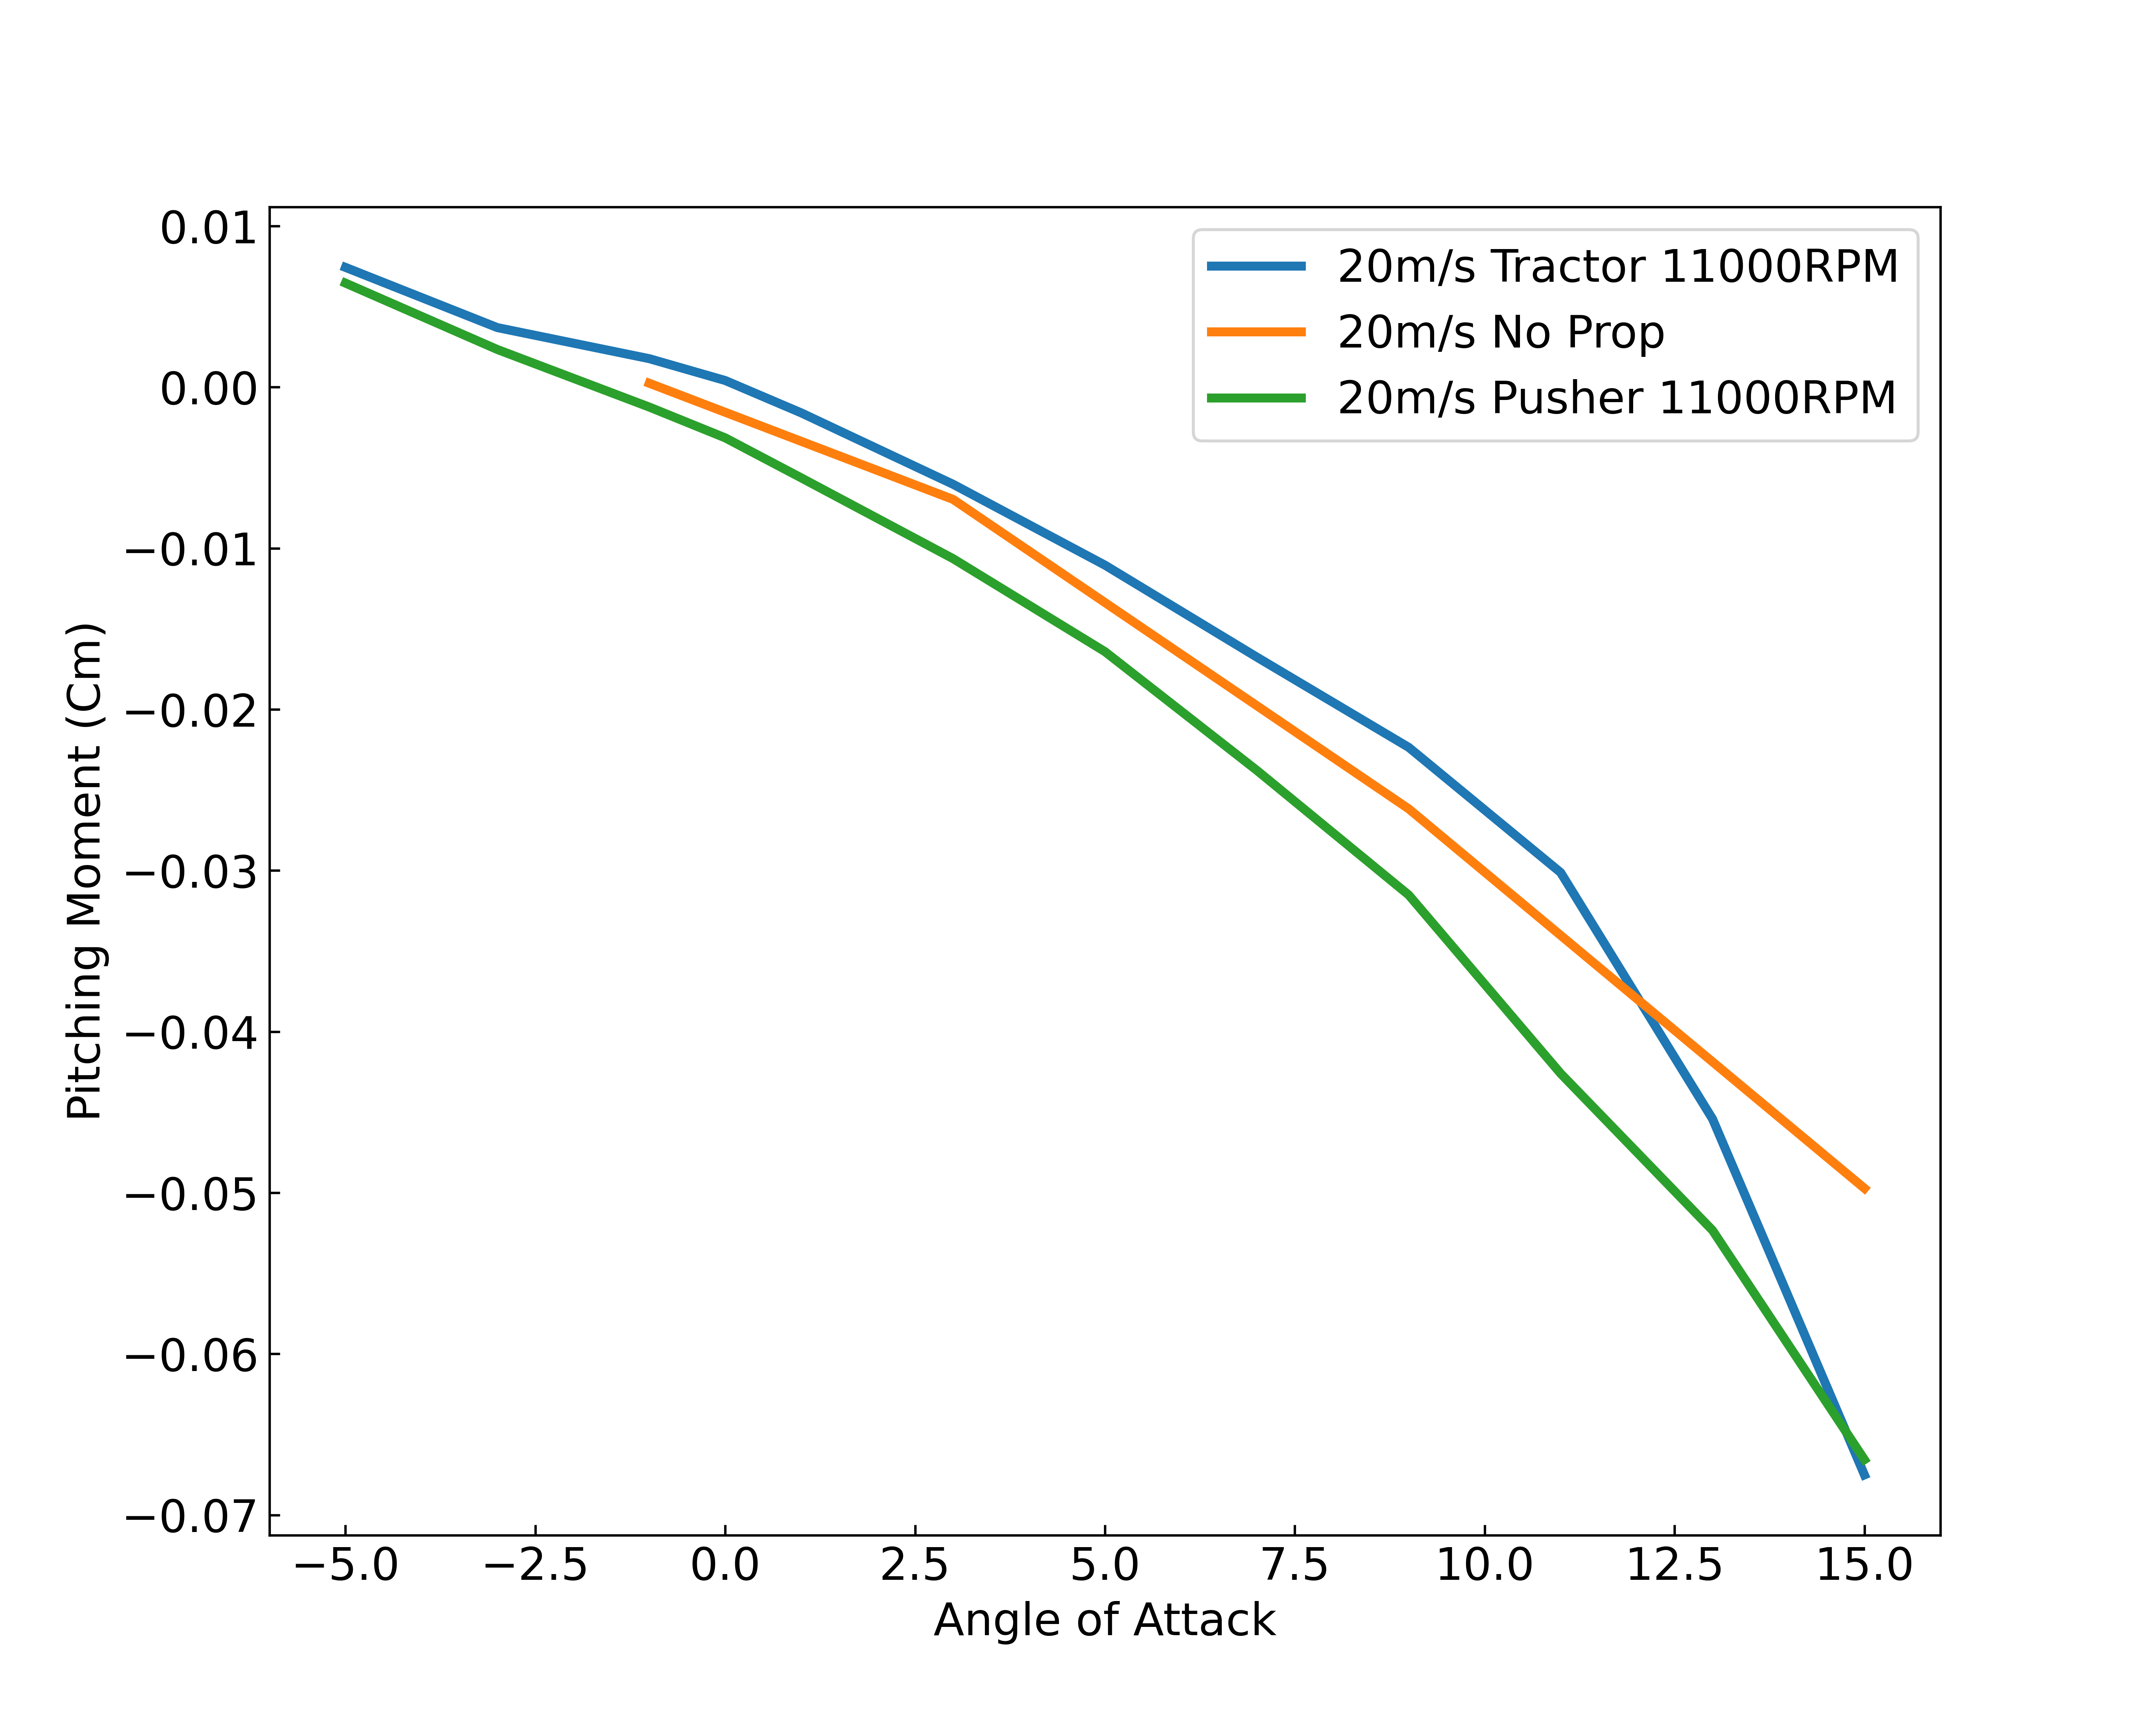
\includegraphics[width=\textwidth]{05_Results/Figs/Cm/20ms_11000RPM_Cm.png}
        \caption{Pitching Moment Coefficient at 20m/s airspeed and 11000RPM motor speed}
        \label{fig:Cm_20ms_11000}
    \end{subfigure}
    \label{fig:Cm_graphs}
\end{figure}



\subsection{Yawing Moment Coefficient}
The yawing coefficient was larger for the tractor configuration due to a larger moment arm 

\begin{figure}[H]
    \centering
    \begin{subfigure}[b]{0.467\textwidth}
        \centering
        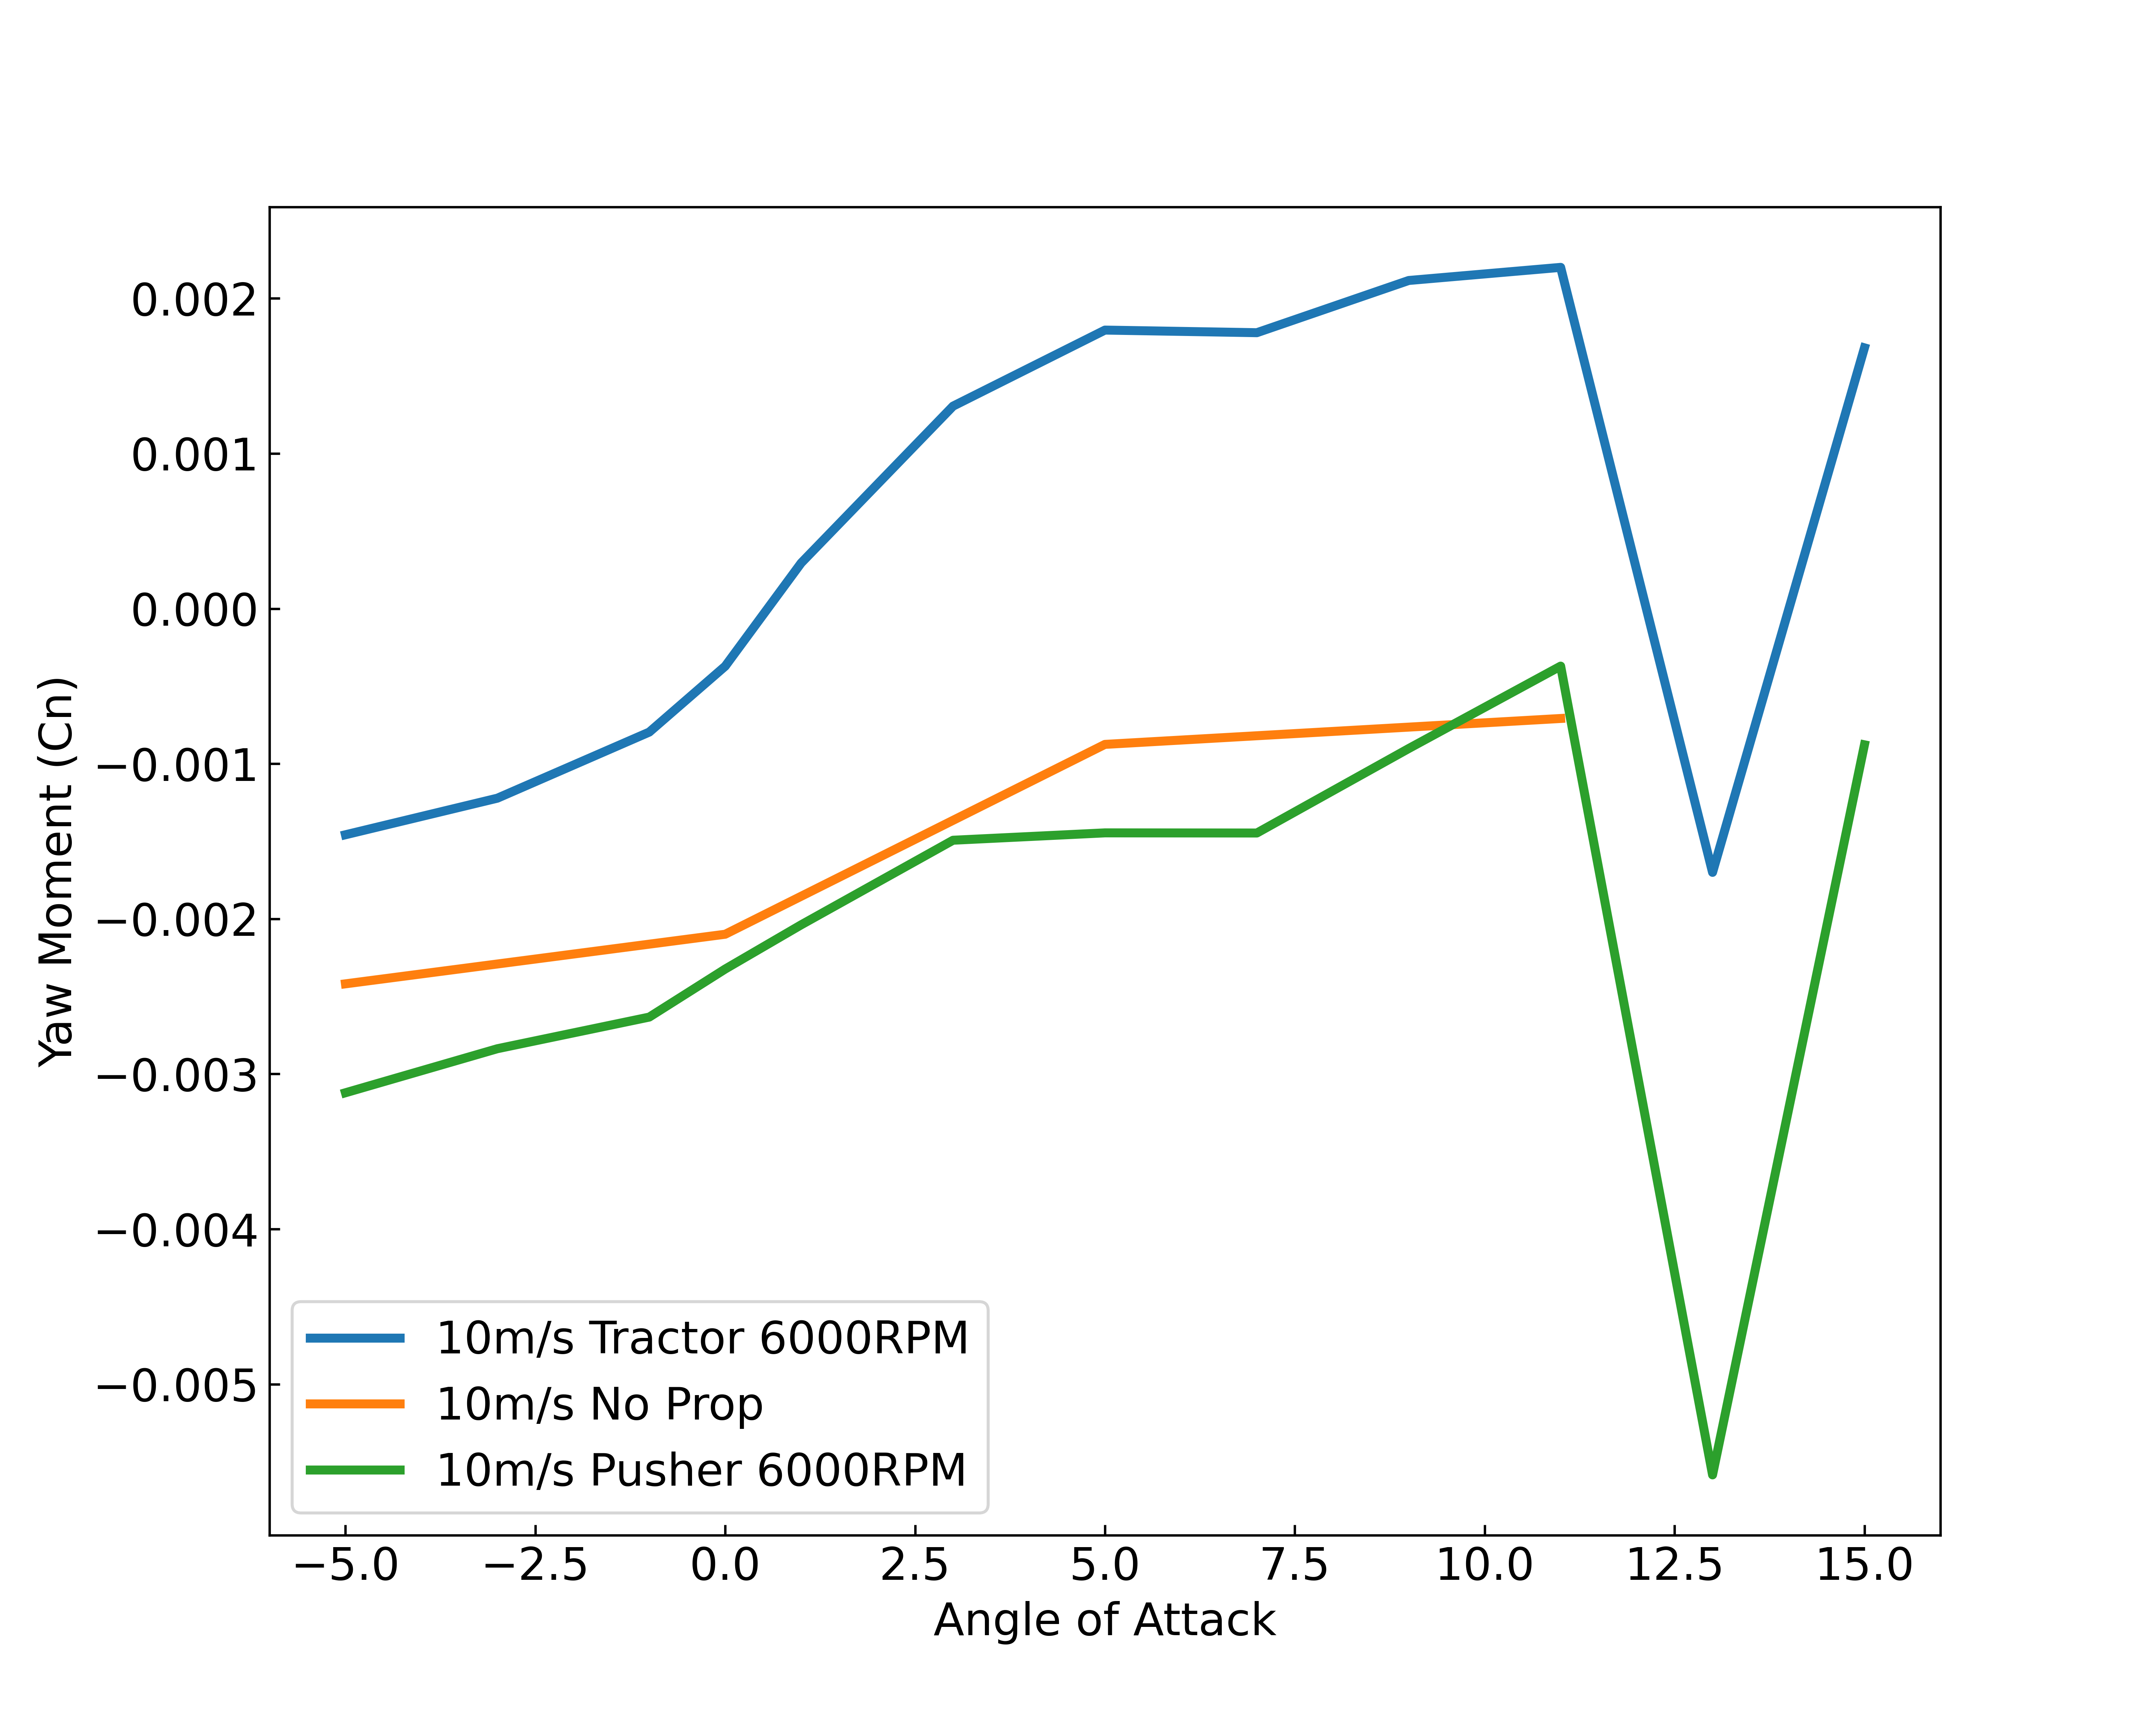
\includegraphics[width=\textwidth]{05_Results/Figs/Cn/10ms_6000RPM_Cn.png}
        \caption{Yawing Moment Coefficient at 10m/s airspeed and 6000RPM motor speed}
        \label{fig:Cn_10ms_6000}
    \end{subfigure}
    \begin{subfigure}[b]{0.467\textwidth}
        \centering
        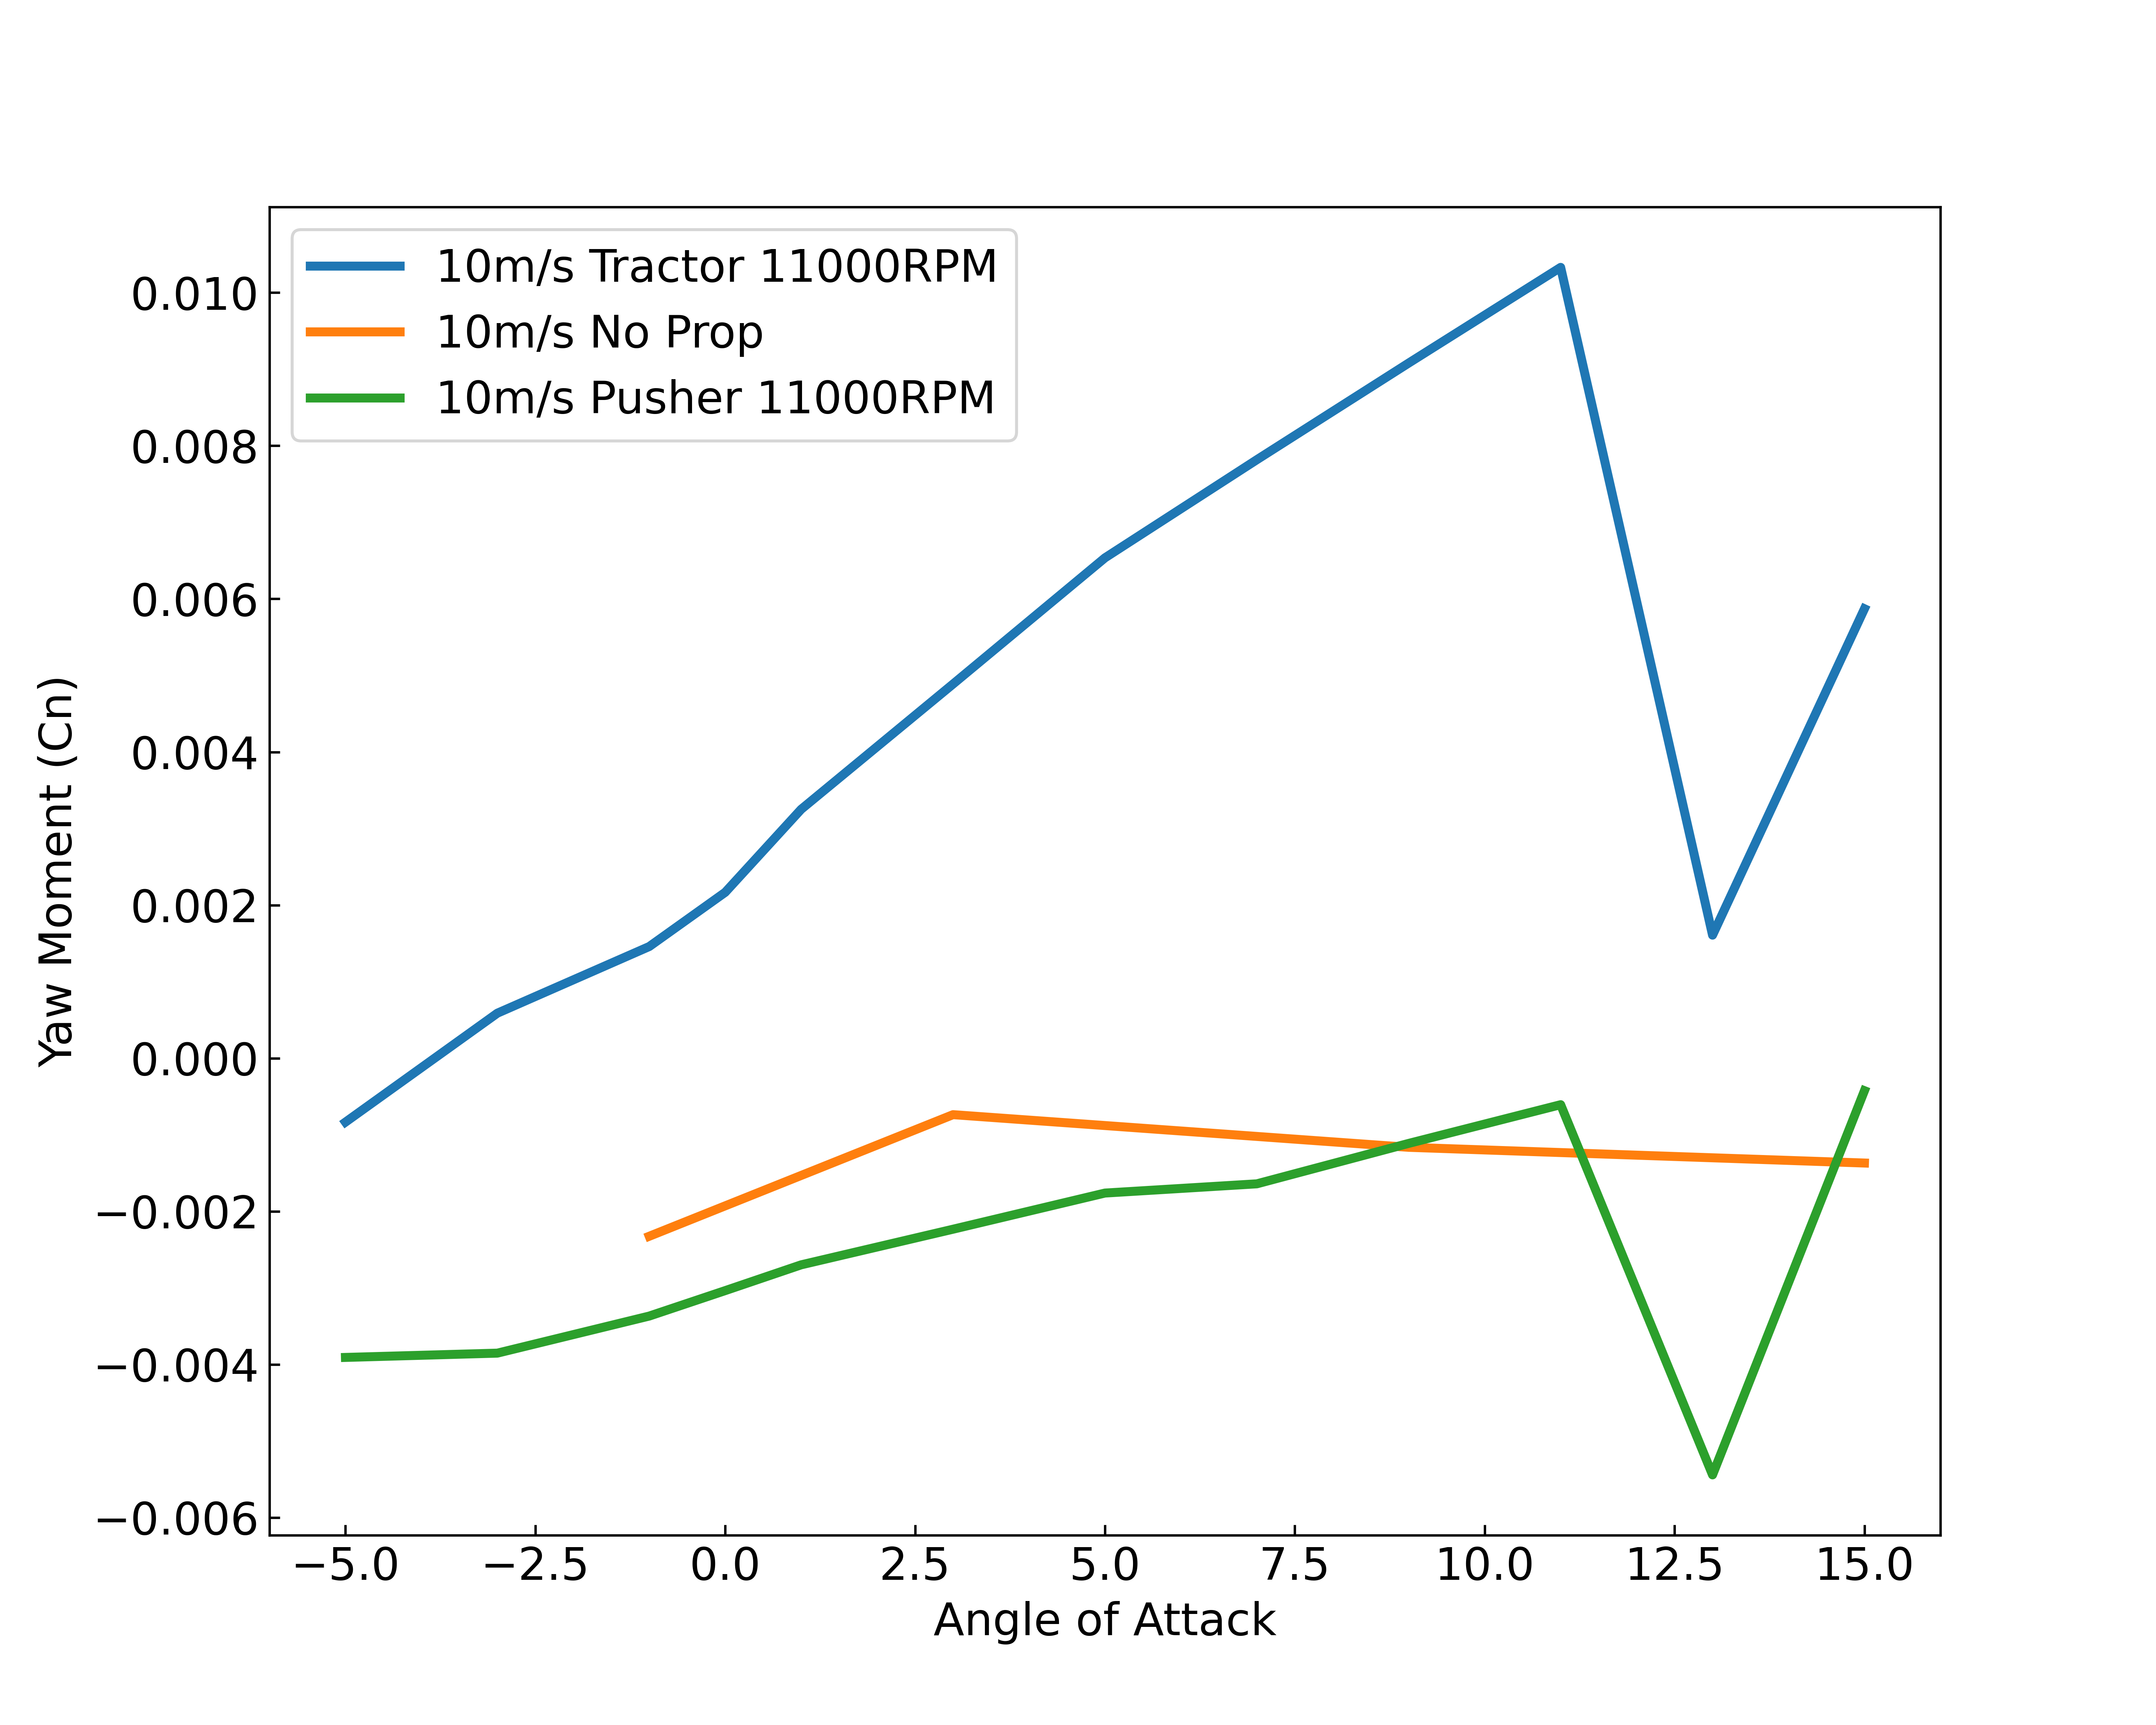
\includegraphics[width=\textwidth]{05_Results/Figs/Cn/10ms_11000RPM_Cn.png}
        \caption{Yawing Moment Coefficient at 10m/s airspeed and 11000RPM motor speed}
        \label{fig:Cn_10ms_11000}
    \end{subfigure}
    \begin{subfigure}[b]{0.467\textwidth}
        \centering
        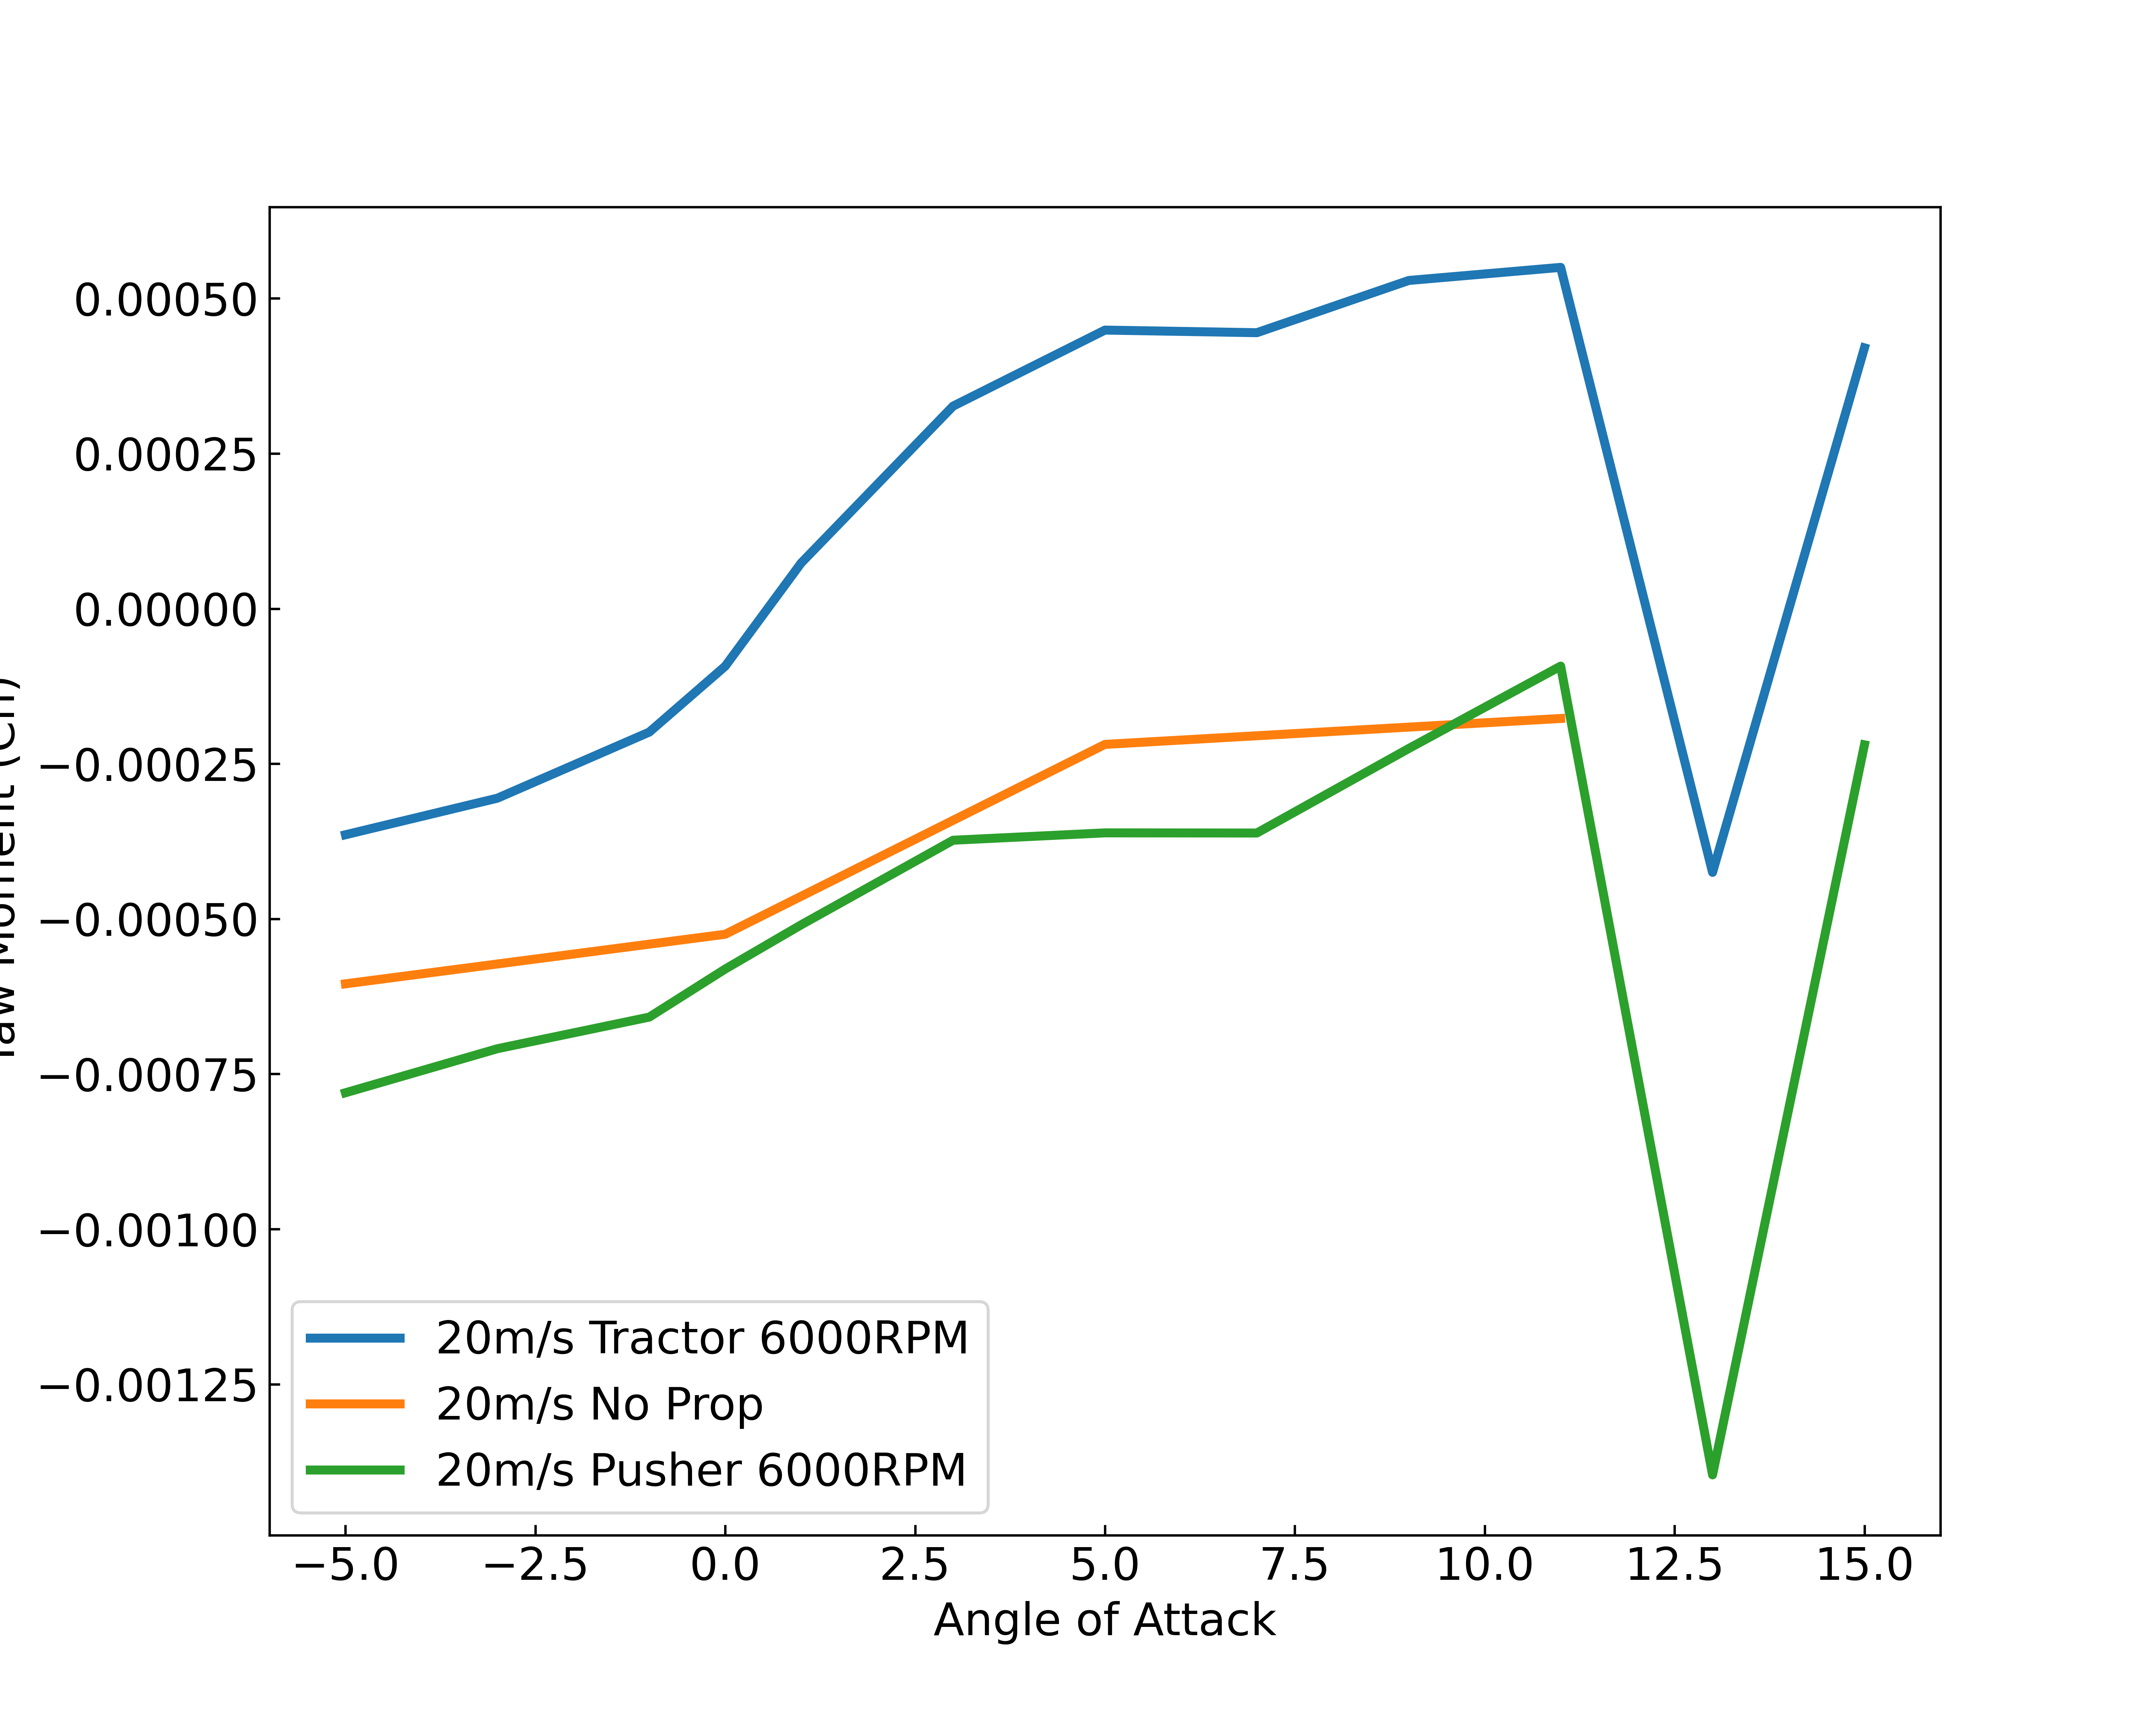
\includegraphics[width=\textwidth]{05_Results/Figs/Cn/20ms_6000RPM_Cn.png}
        \caption{Yawing Moment Coefficient at 20m/s airspeed and 6000RPM motor speed}
        \label{fig:Cn_20ms_6000}
    \end{subfigure}
    \begin{subfigure}[b]{0.467\textwidth}
        \centering
        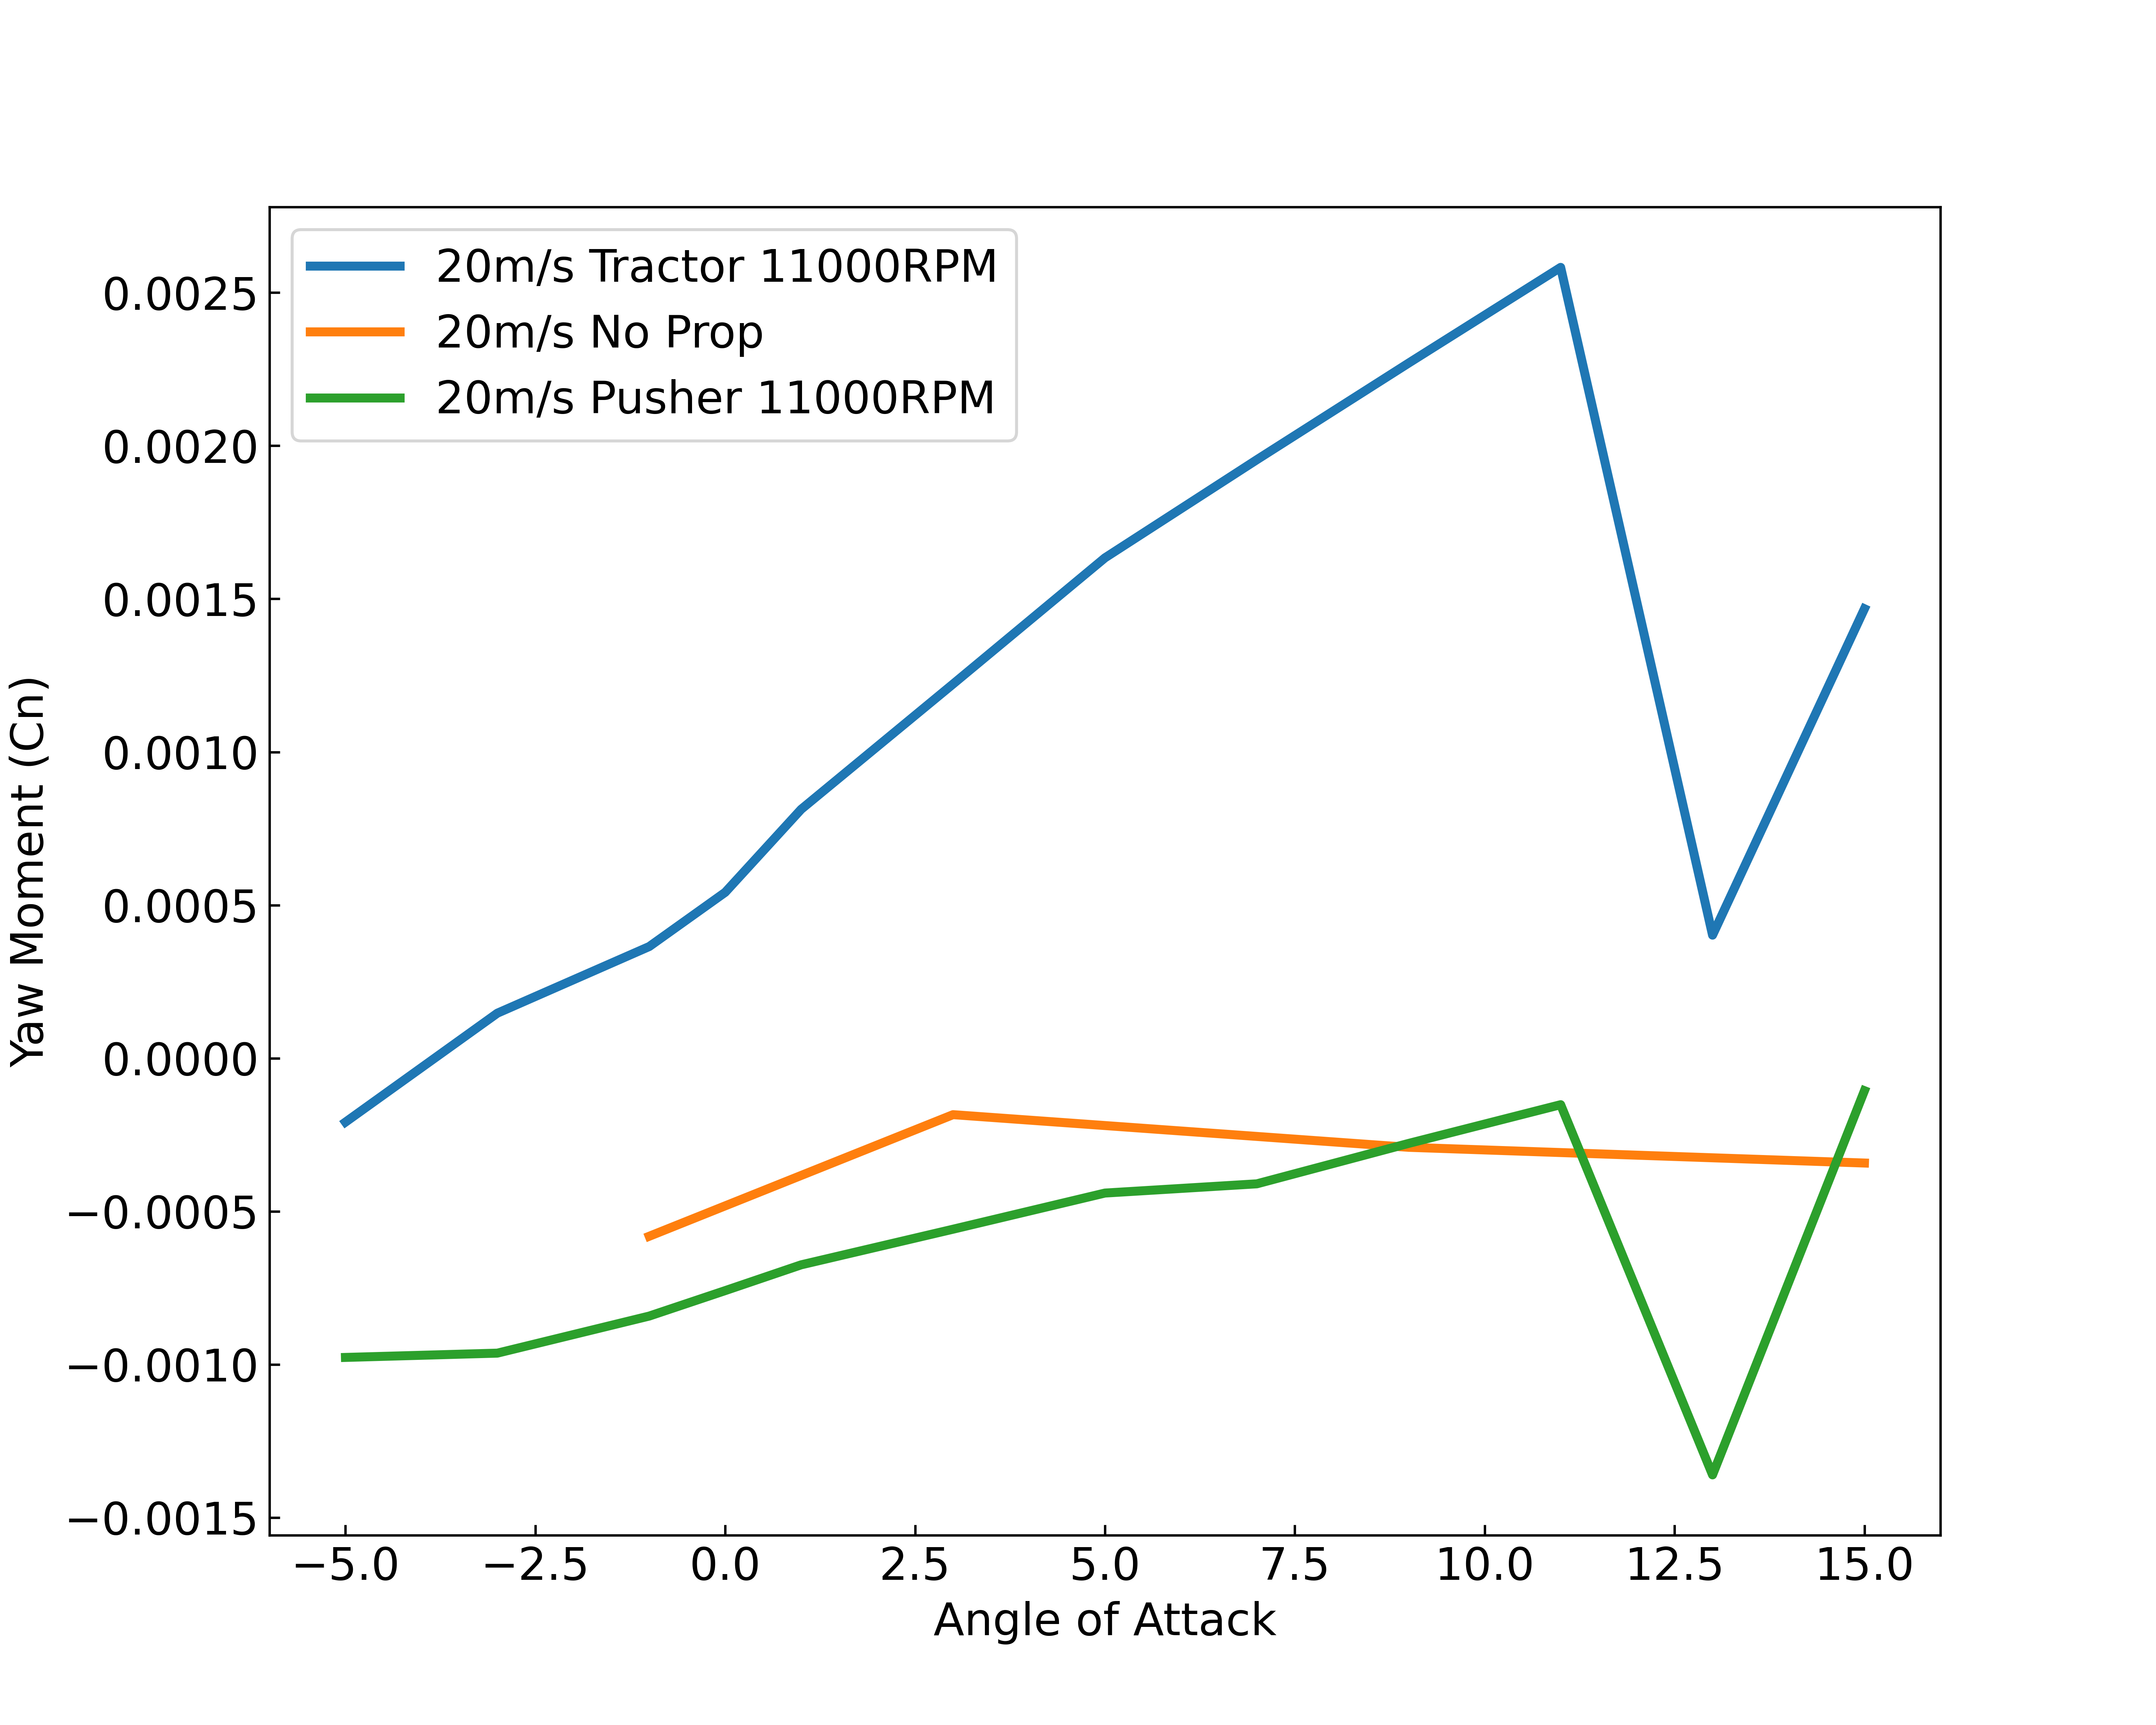
\includegraphics[width=\textwidth]{05_Results/Figs/Cn/20ms_11000RPM_Cn.png}
        \caption{Yawing Moment Coefficient at 20m/s airspeed and 11000RPM motor speed}
        \label{fig:Cn_20ms_11000}
    \end{subfigure}
\end{figure}


\subsection{Rolling Moment Coefficient}

\begin{figure}[H]
    \centering
    \begin{subfigure}[b]{0.467\textwidth}
        \centering
        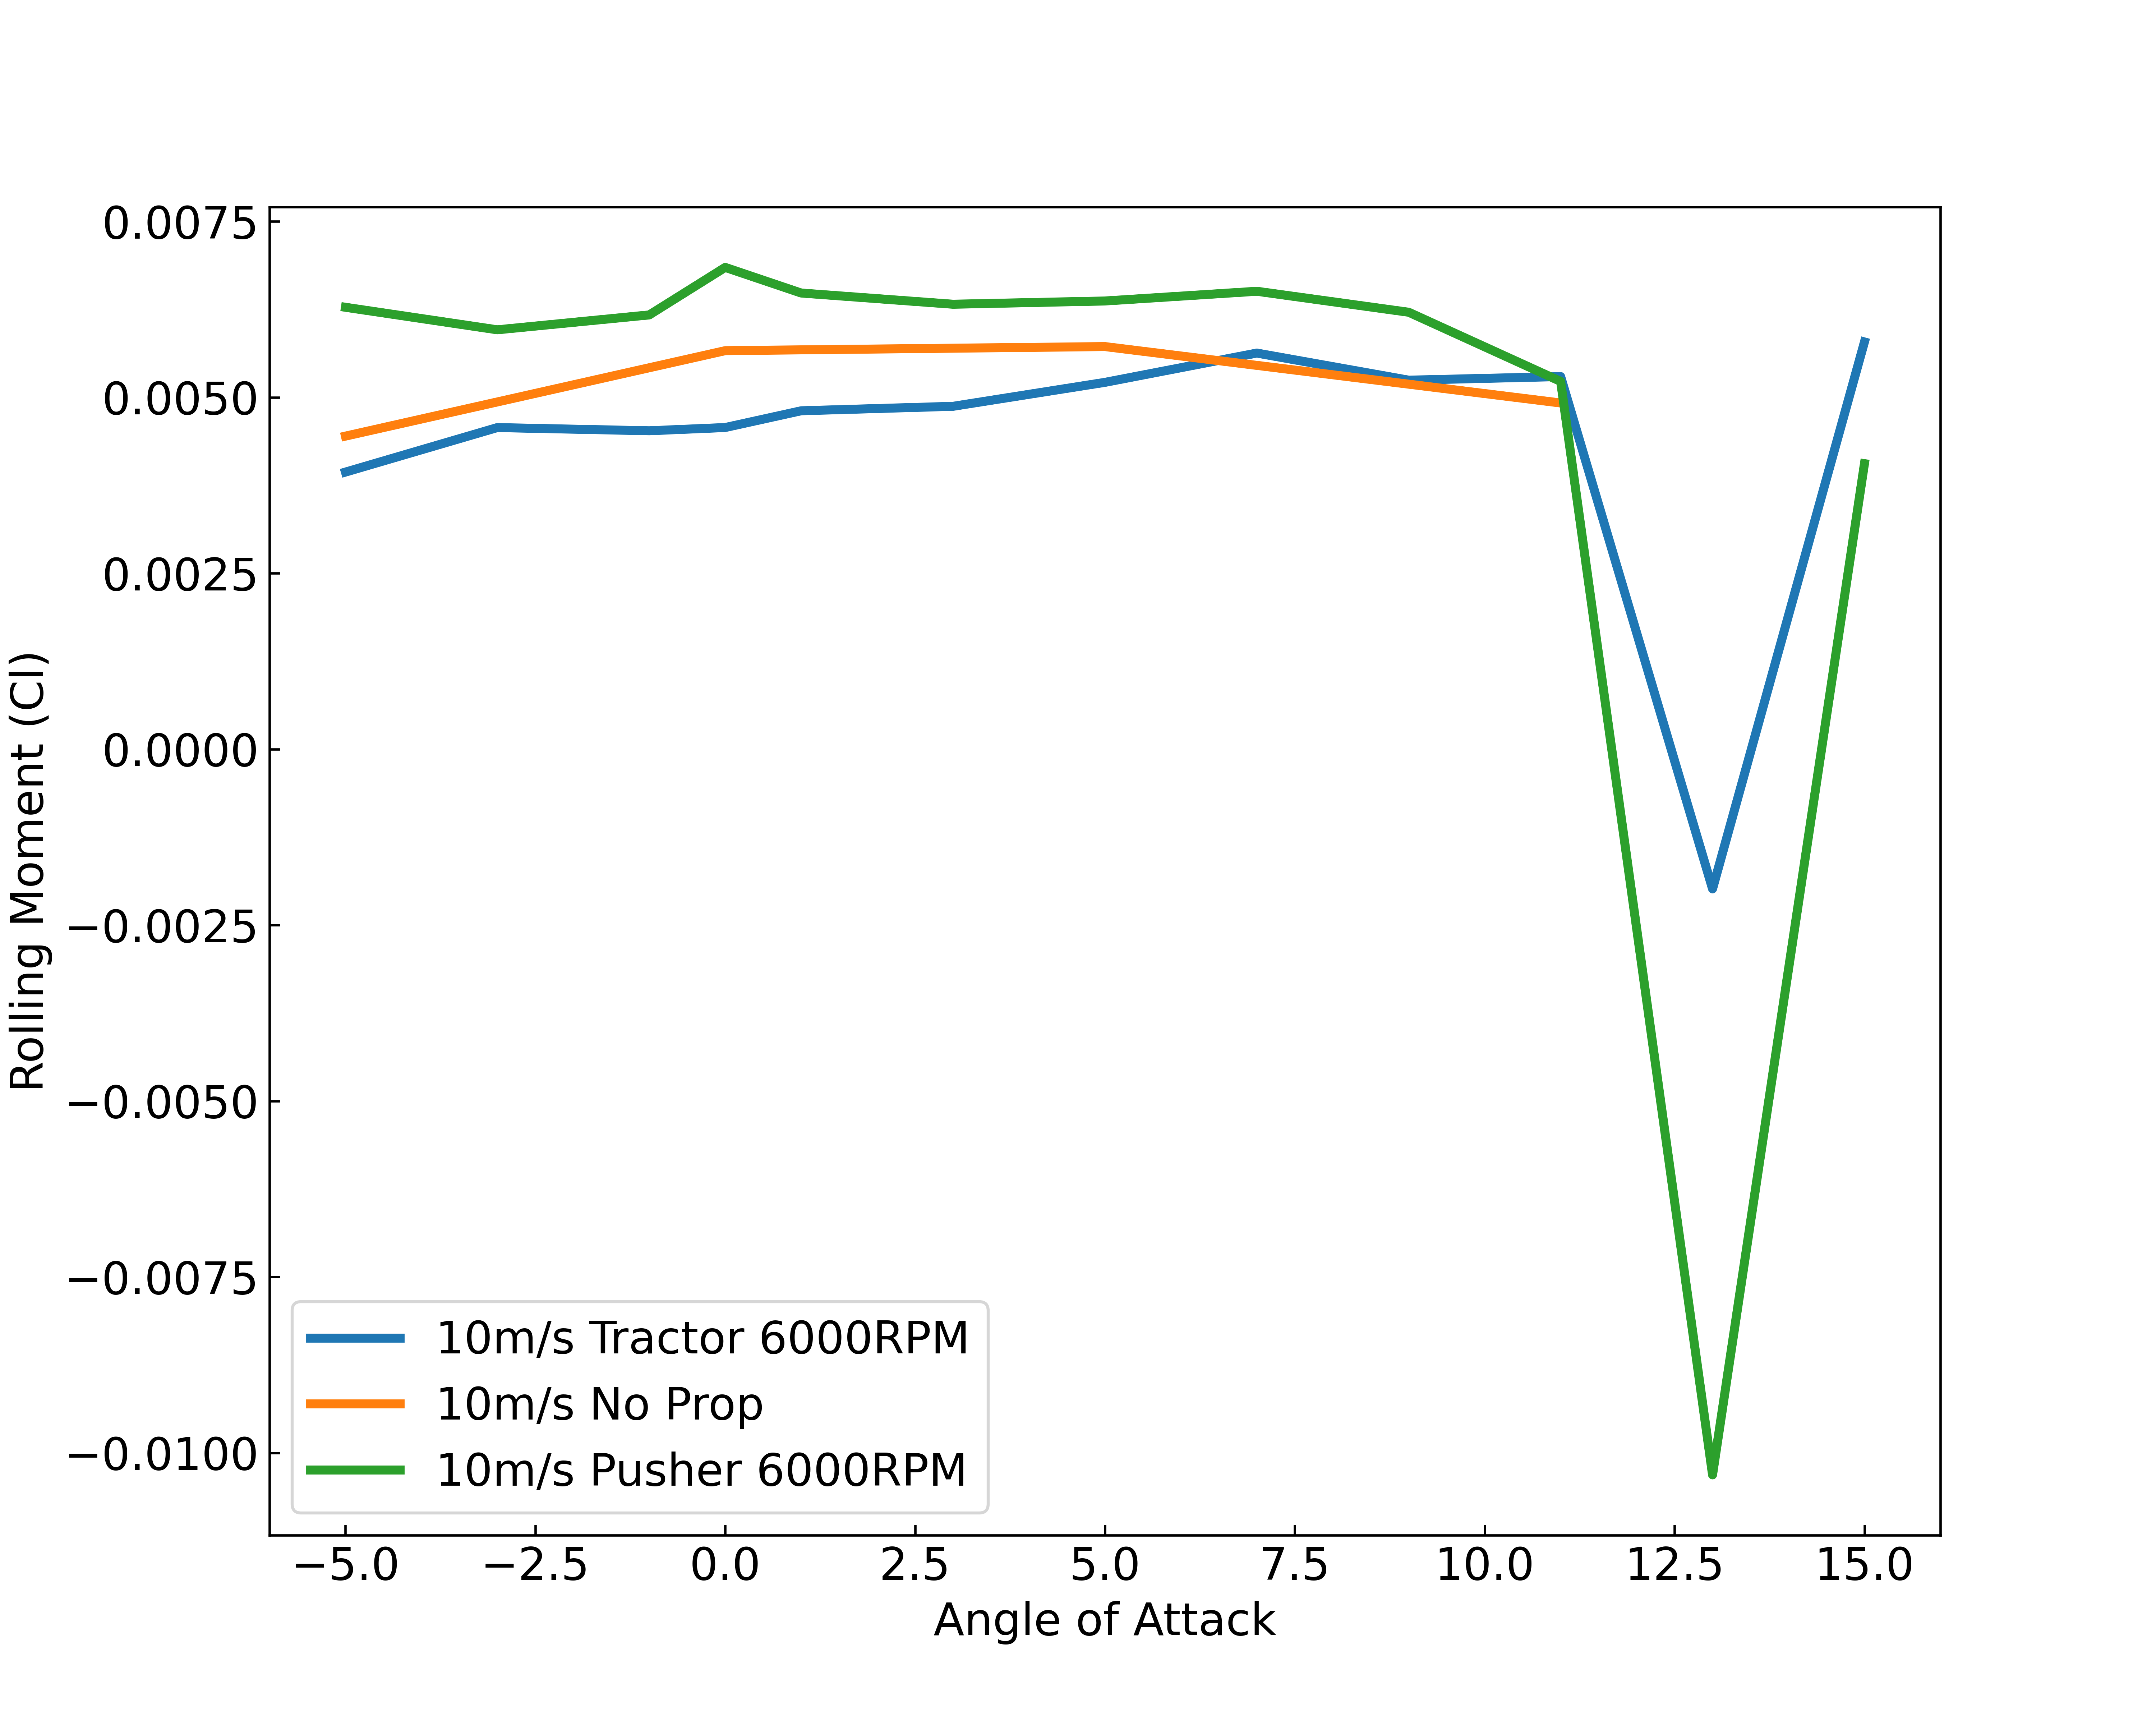
\includegraphics[width=\textwidth]{05_Results/Figs/Cl_roll/10ms_6000RPM_Cl_roll.png}
        \caption{Rolling Moment Coefficient at 10m/s airspeed and 6000RPM motor speed}
        \label{fig:Cl_roll_10ms_6000}
    \end{subfigure}
    \begin{subfigure}[b]{0.467\textwidth}
        \centering
        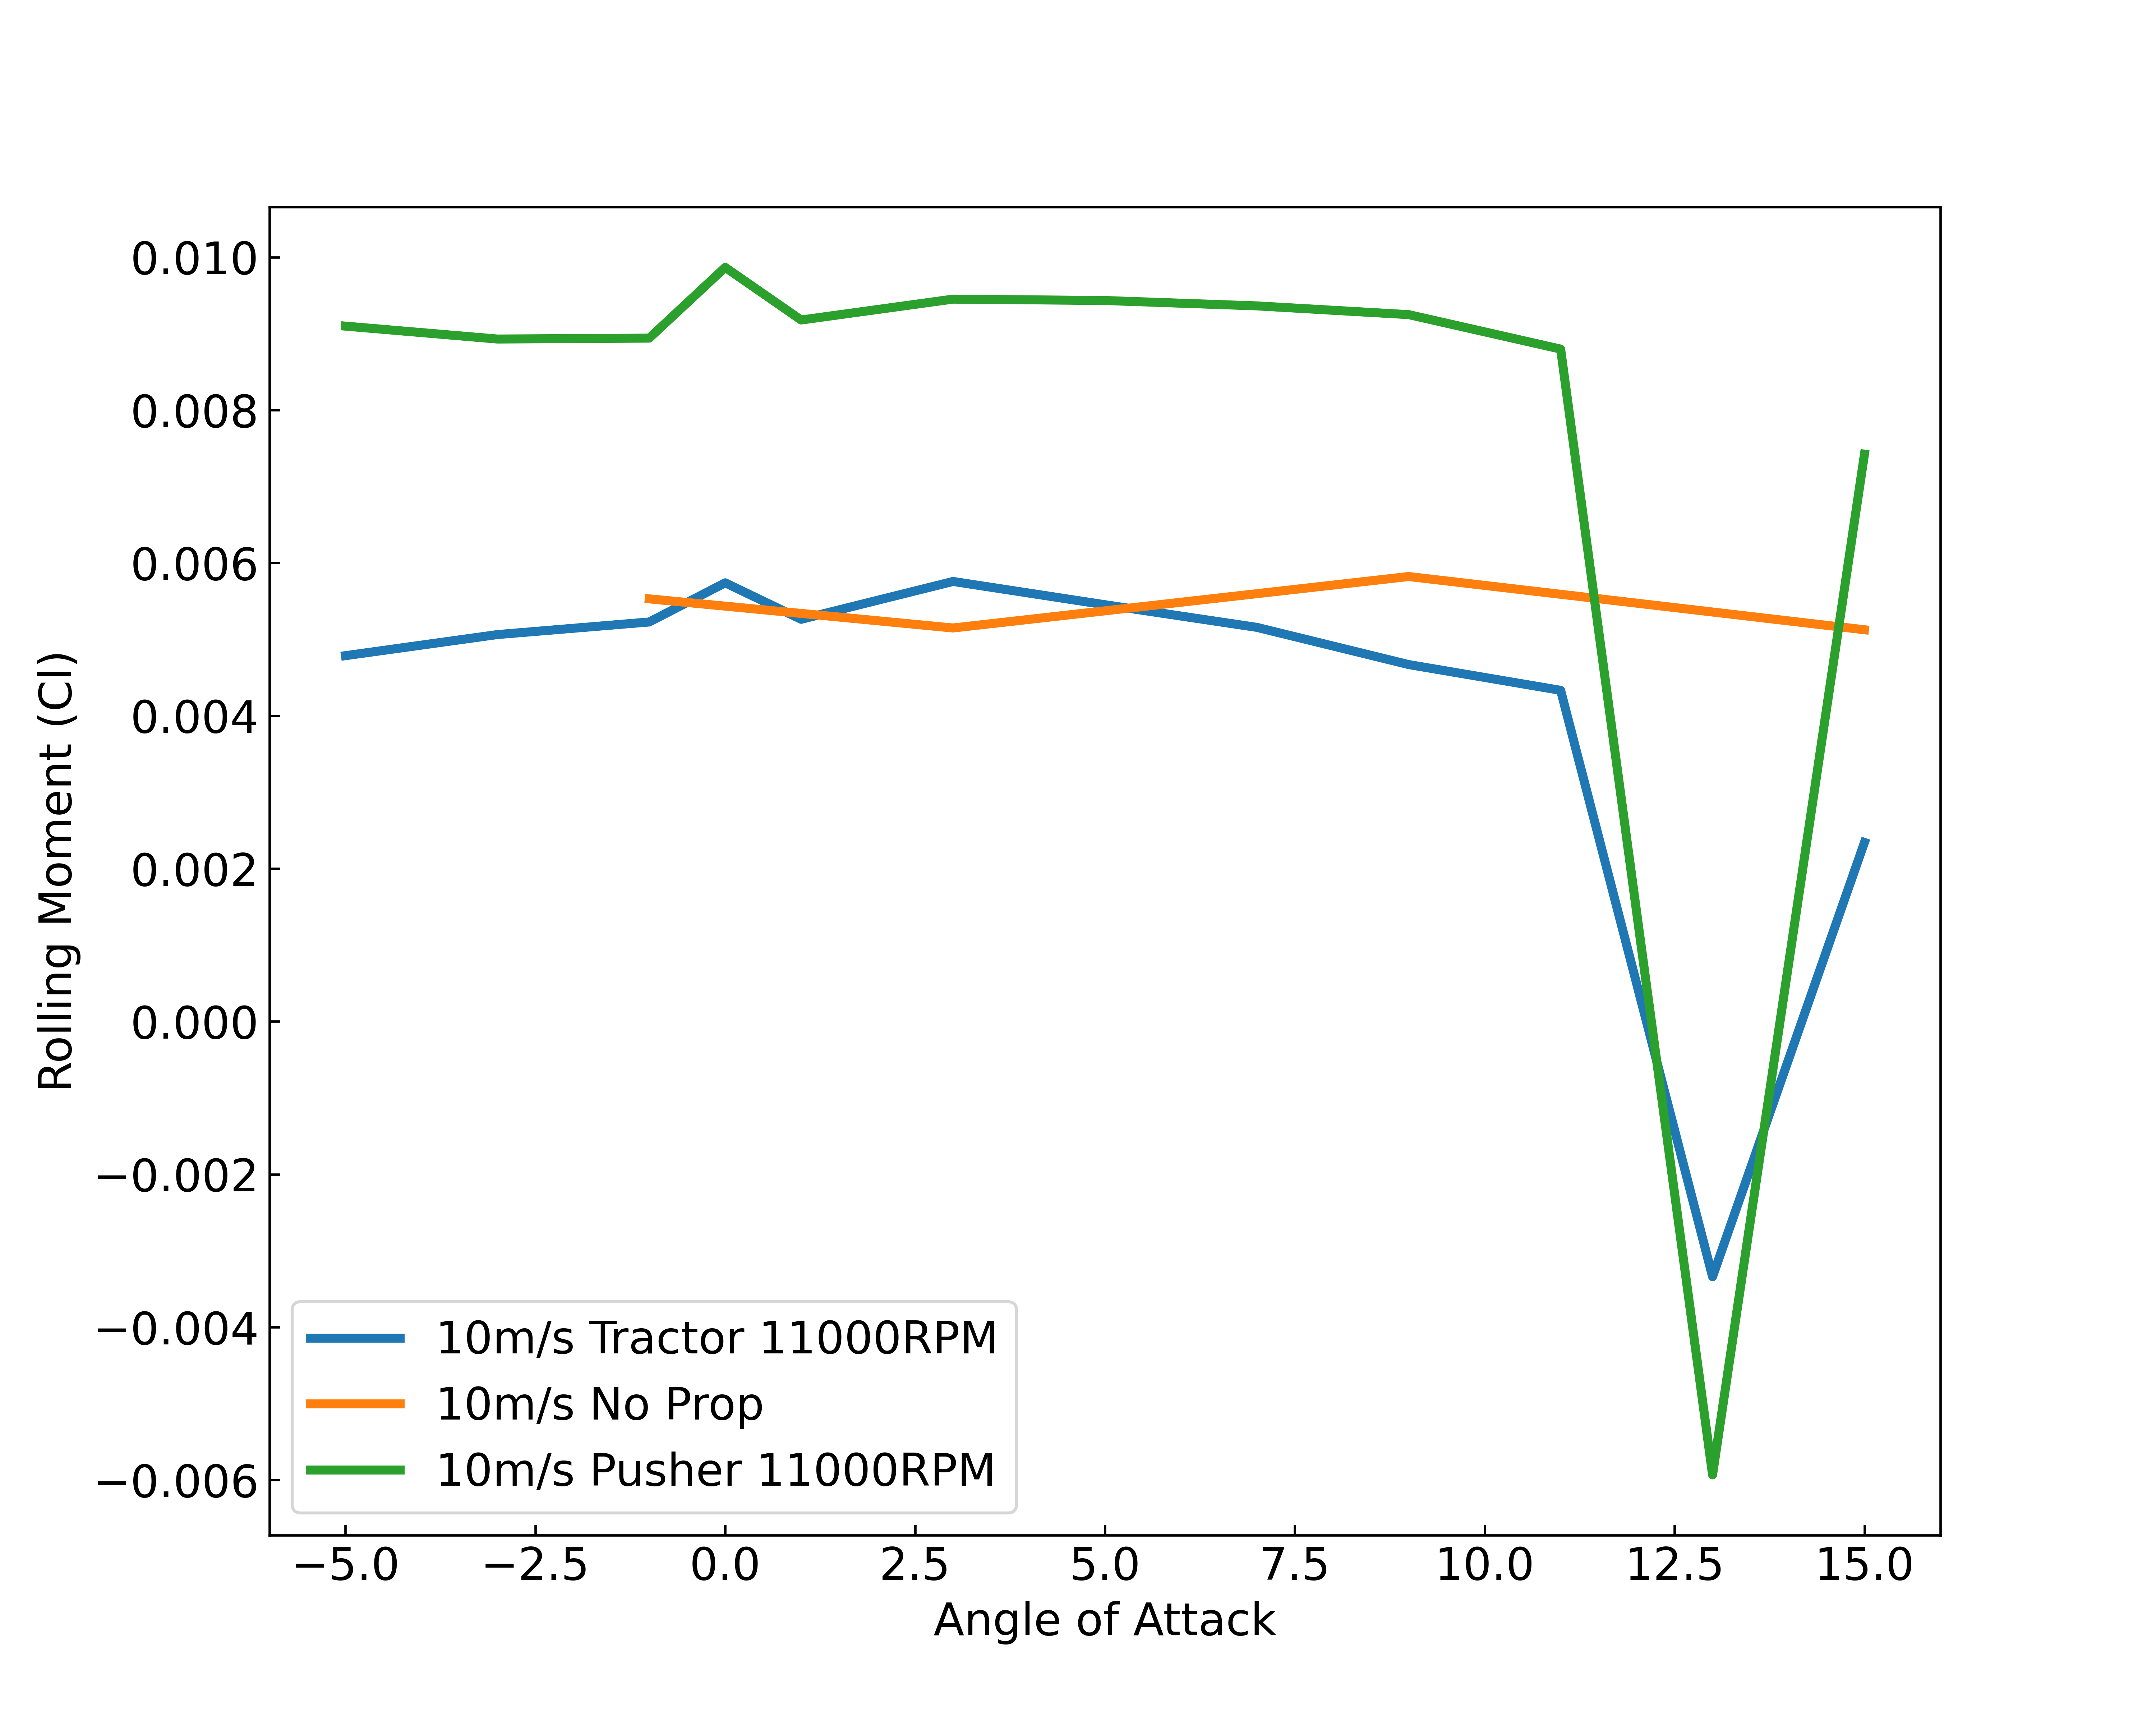
\includegraphics[width=\textwidth]{05_Results/Figs/Cl_roll/10ms_11000RPM_Cl.png}
        \caption{Rolling Moment Coefficient at 10m/s airspeed and 11000RPM motor speed}
        \label{fig:Cl_roll_10ms_11000}
    \end{subfigure}
    \begin{subfigure}[b]{0.467\textwidth}
        \centering
        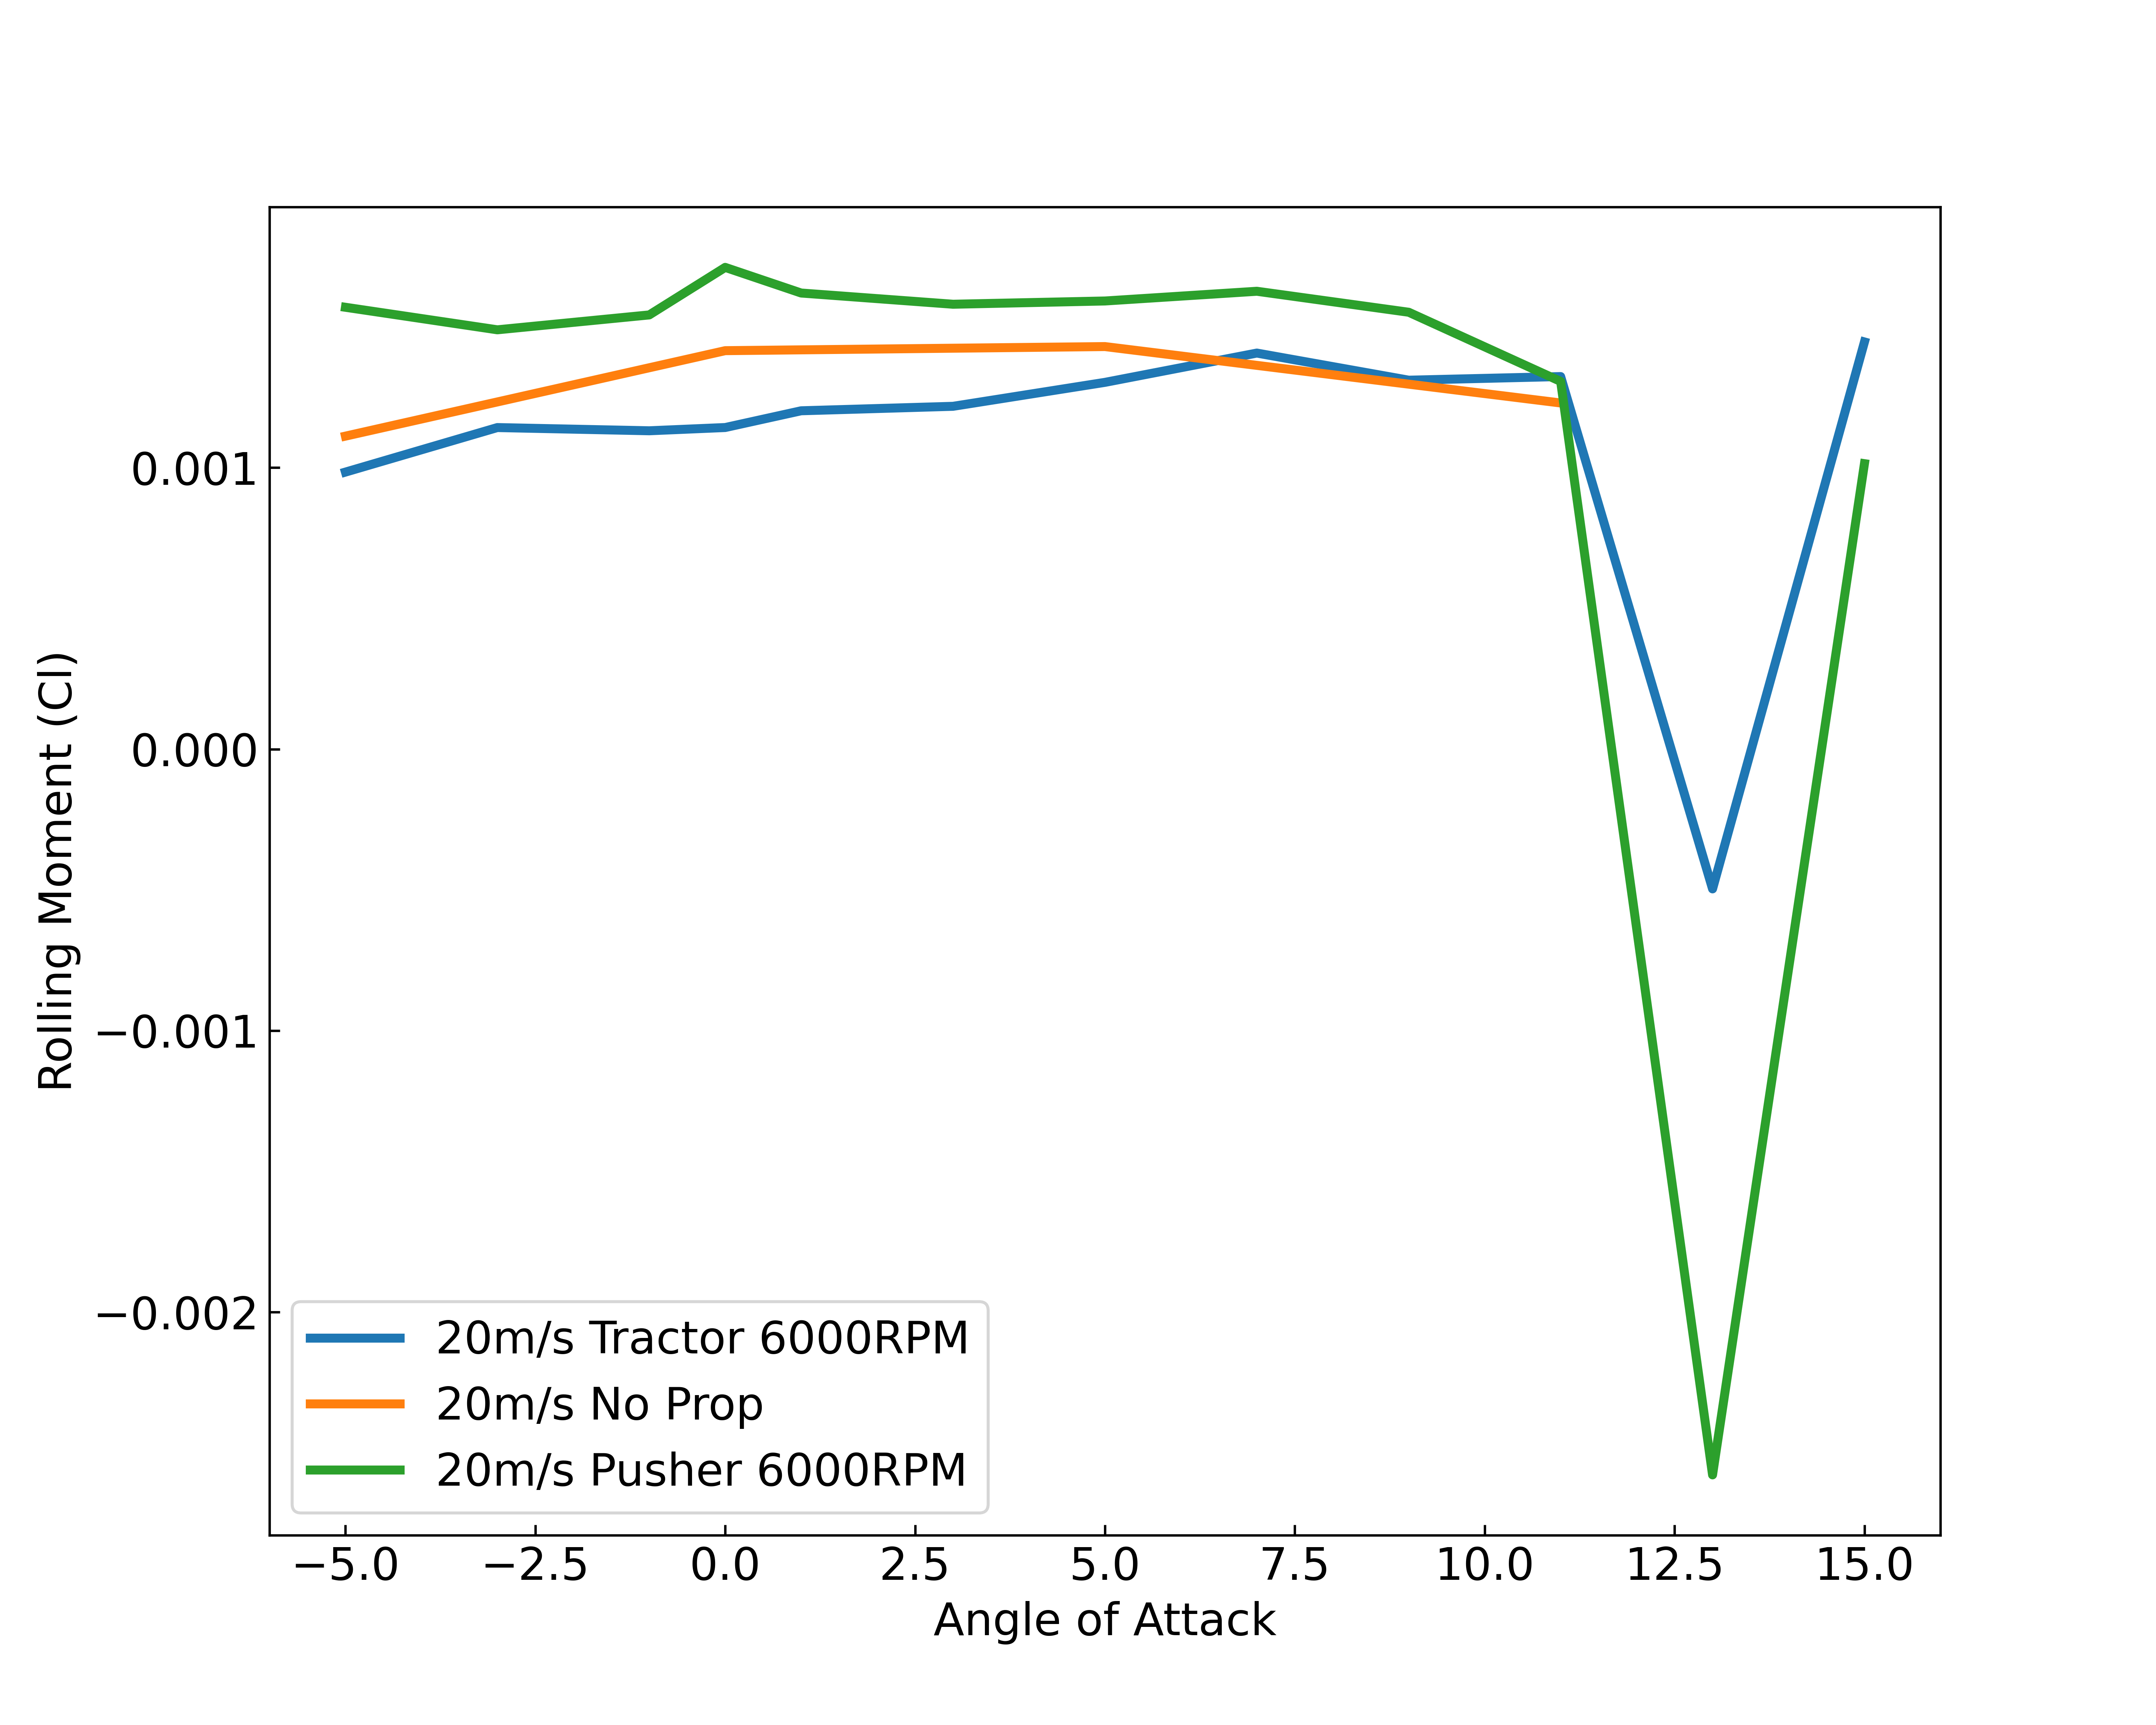
\includegraphics[width=\textwidth]{05_Results/Figs/Cl_roll/20ms_6000RPM_Cl_roll.png}
        \caption{Rolling Moment Coefficient at 20m/s airspeed and 6000RPM motor speed}
        \label{fig:Cl_roll_20ms_6000}
    \end{subfigure}
    \begin{subfigure}[b]{0.467\textwidth}
        \centering
        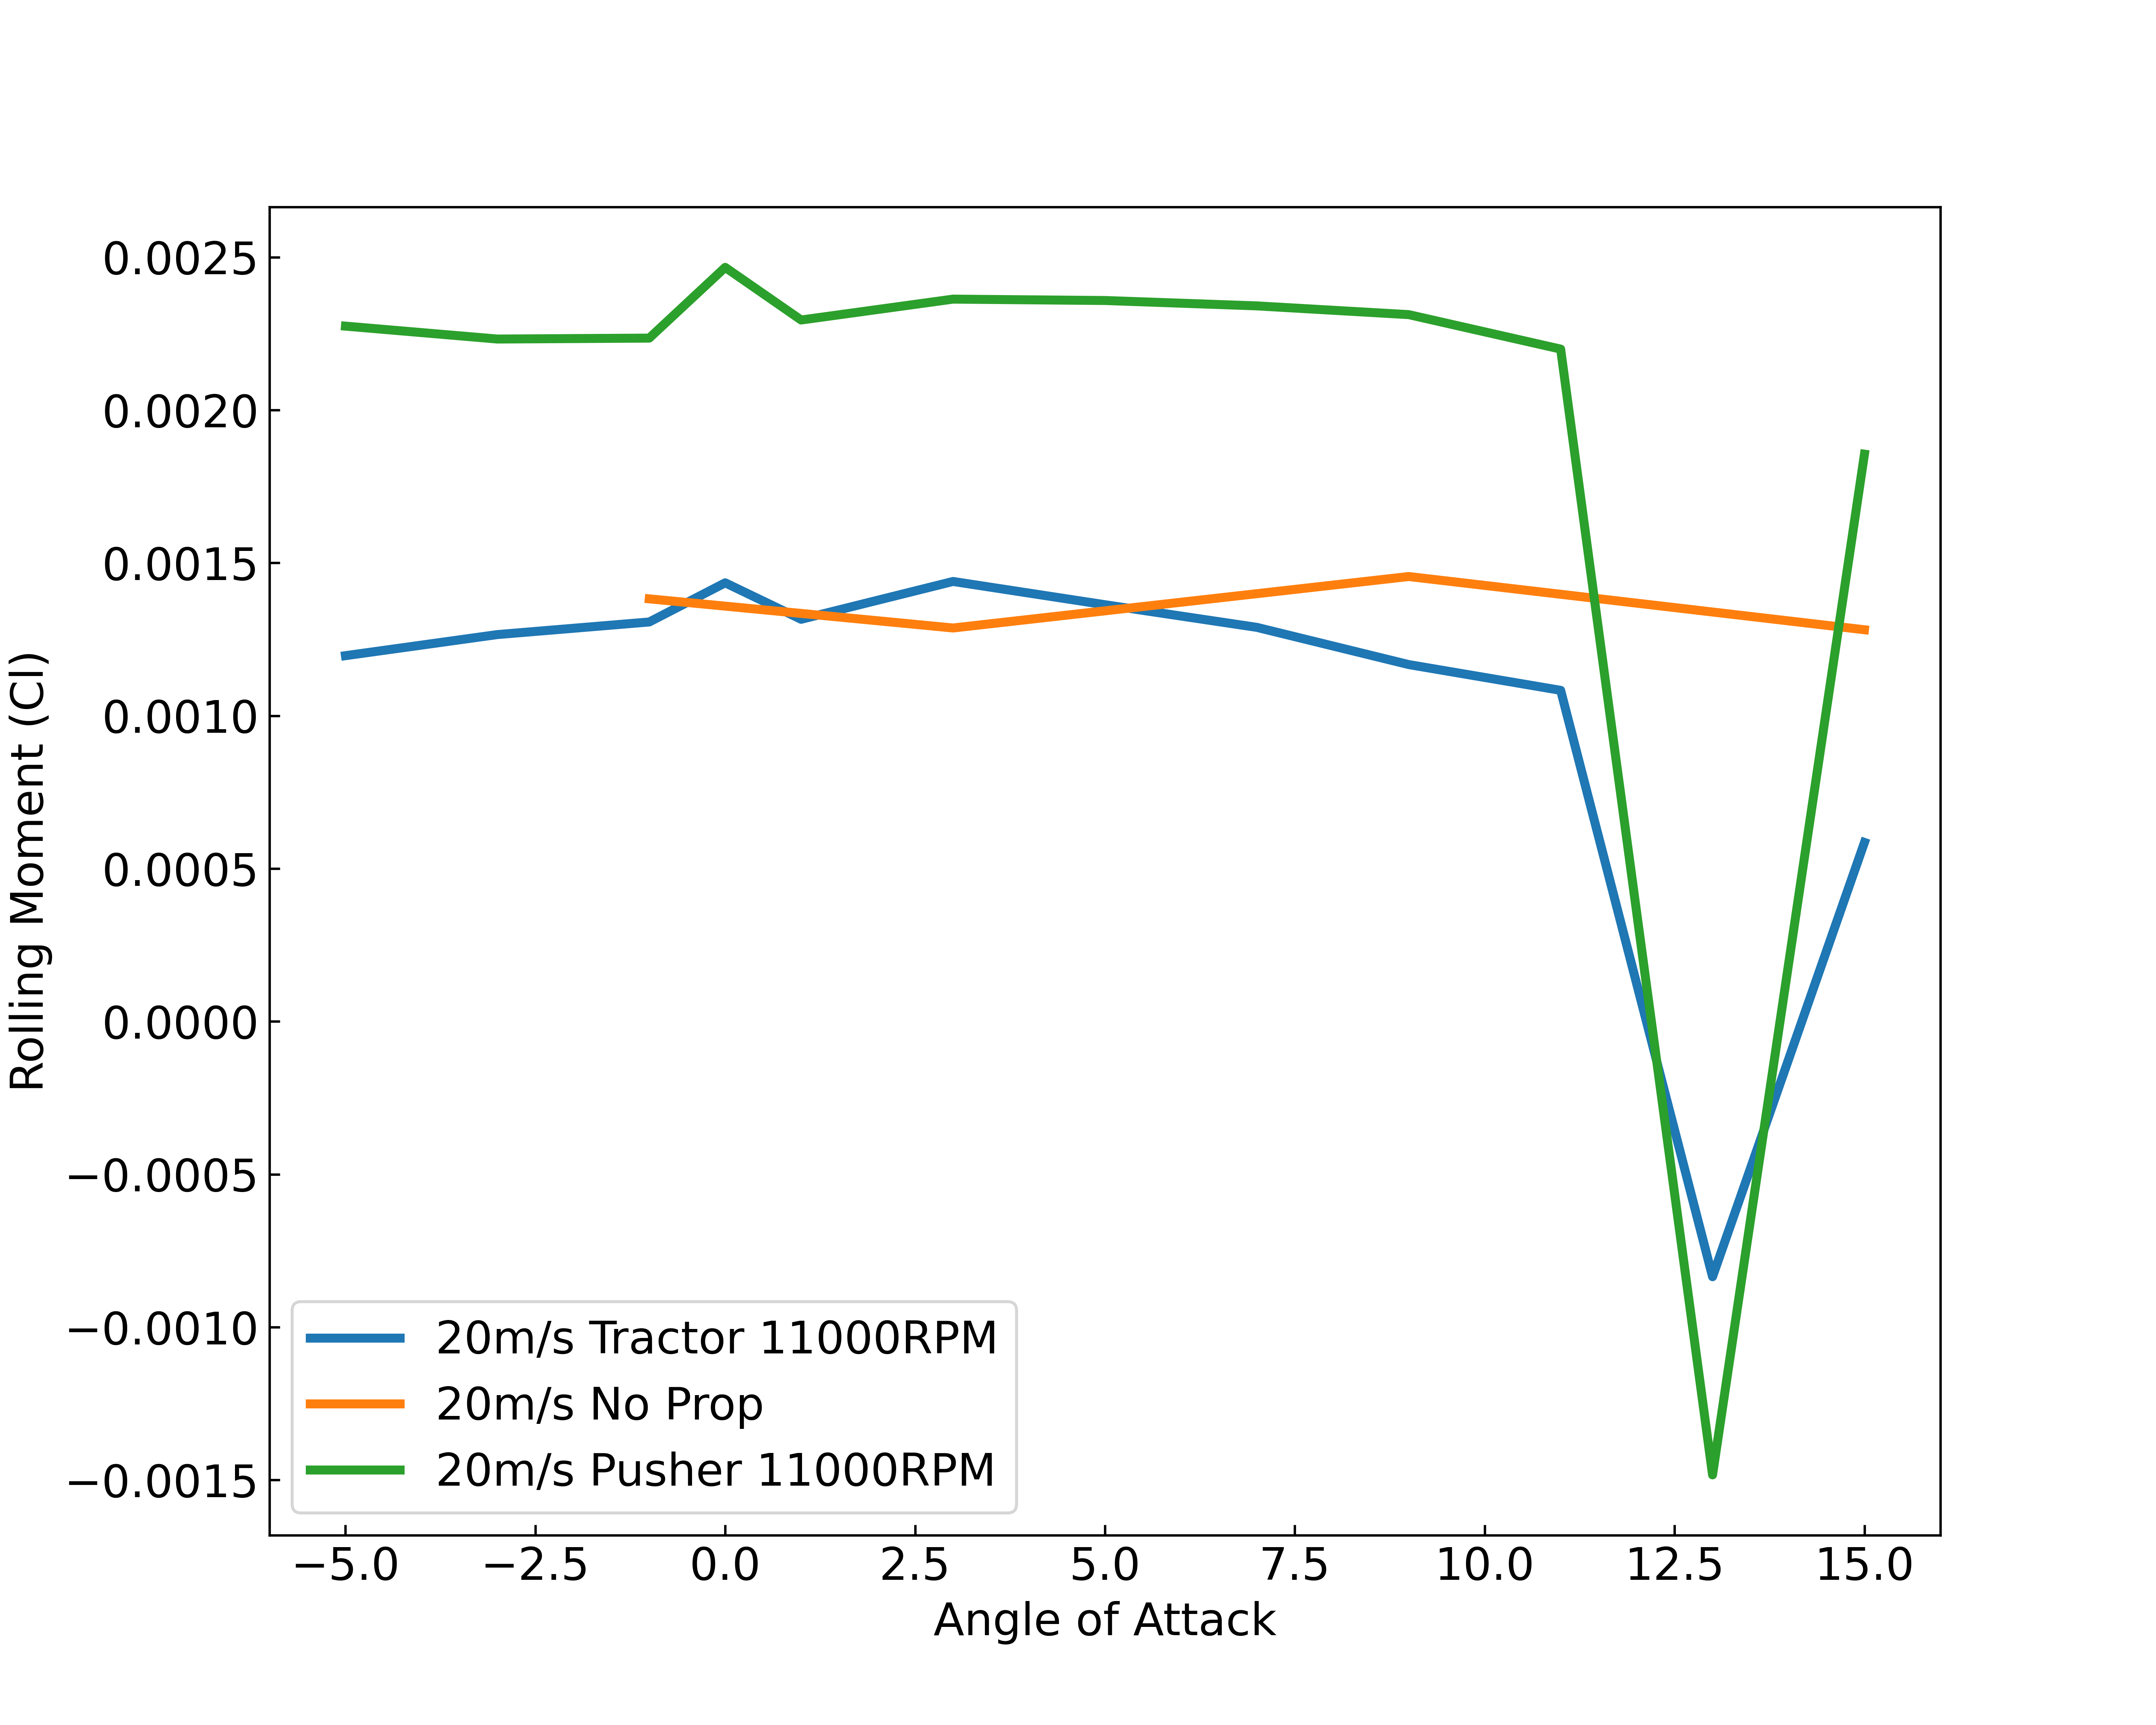
\includegraphics[width=\textwidth]{05_Results/Figs/Cl_roll/20ms_11000RPM_Cl.png}
        \caption{Rolling Moment Coefficient at 20m/s airspeed and 11000RPM motor speed}
        \label{fig:Cl_roll_20ms_11000}
    \end{subfigure}
\end{figure}

\subsection{Static Margin}

\todo{Add table with values of static margin}
\begin{figure}[H]
    \centering
    \begin{subfigure}[b]{0.467\textwidth}
        \centering
        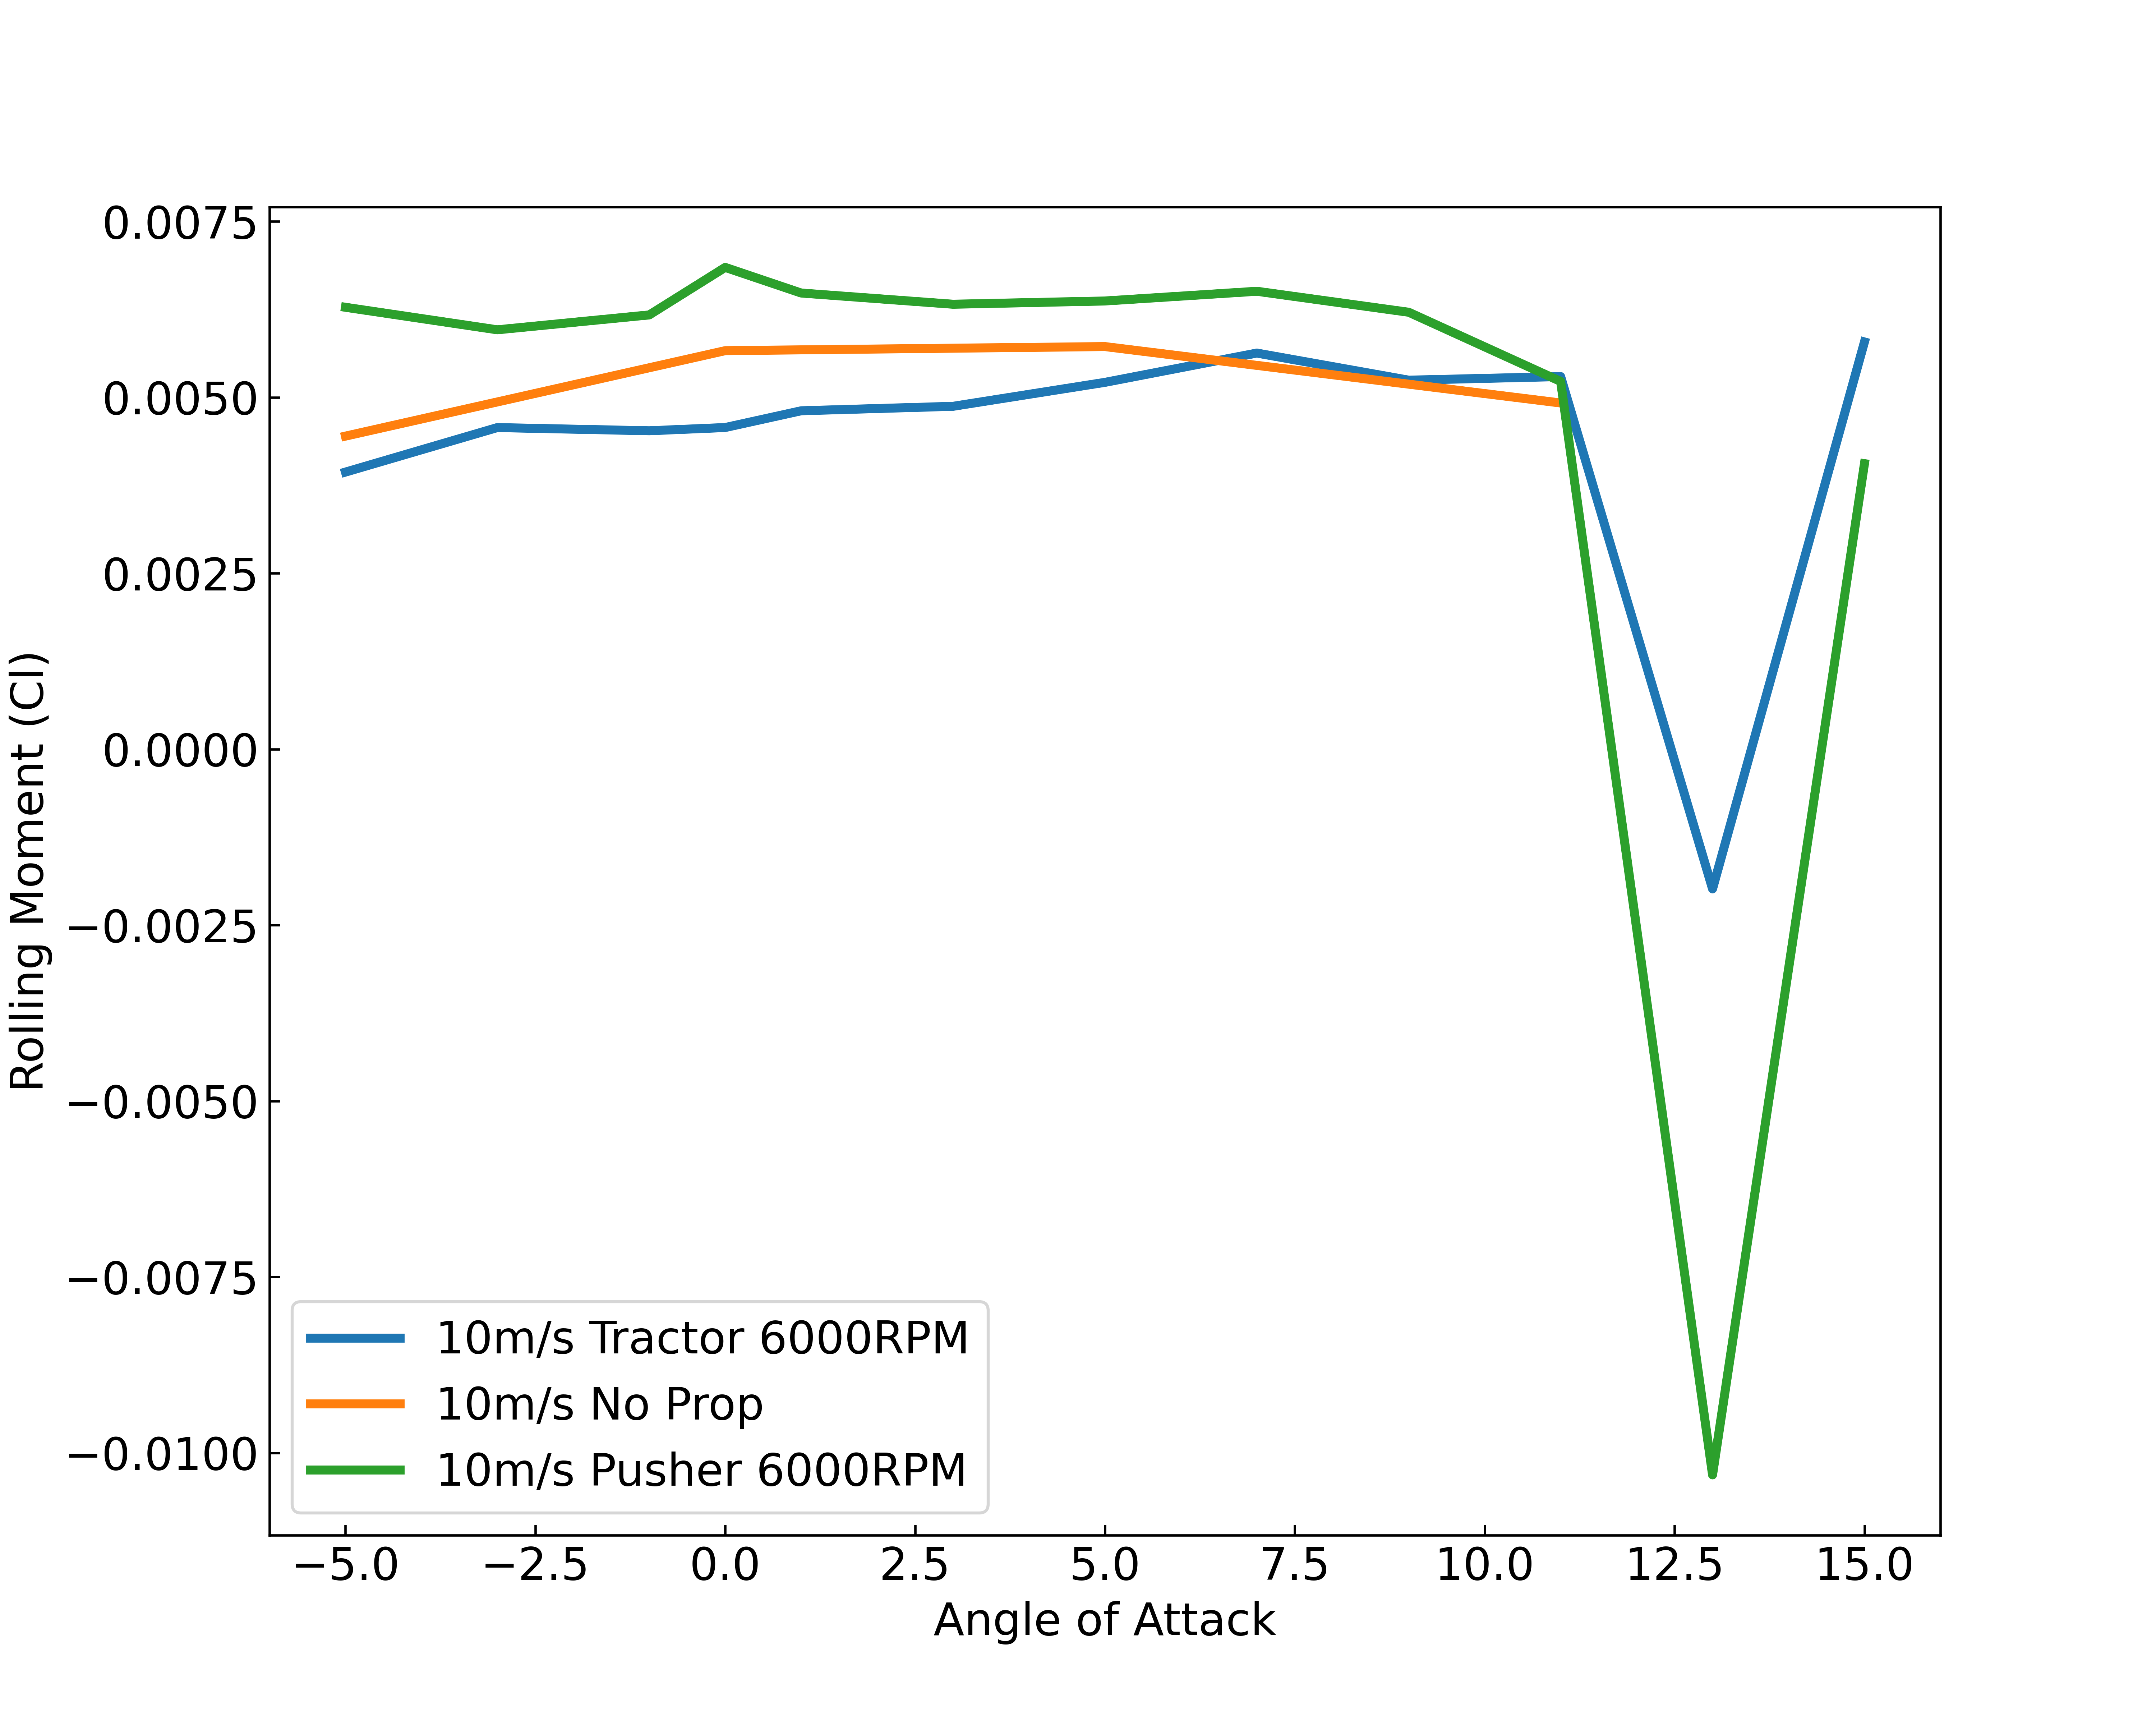
\includegraphics[width=\textwidth]{05_Results/Figs/Cl_roll/10ms_6000RPM_Cl_roll.png}
        \caption{Rolling Moment Coefficient at 10m/s airspeed and 6000RPM motor speed}
        \label{fig:CmCl_10ms_6000}
    \end{subfigure}
    \begin{subfigure}[b]{0.467\textwidth}
        \centering
        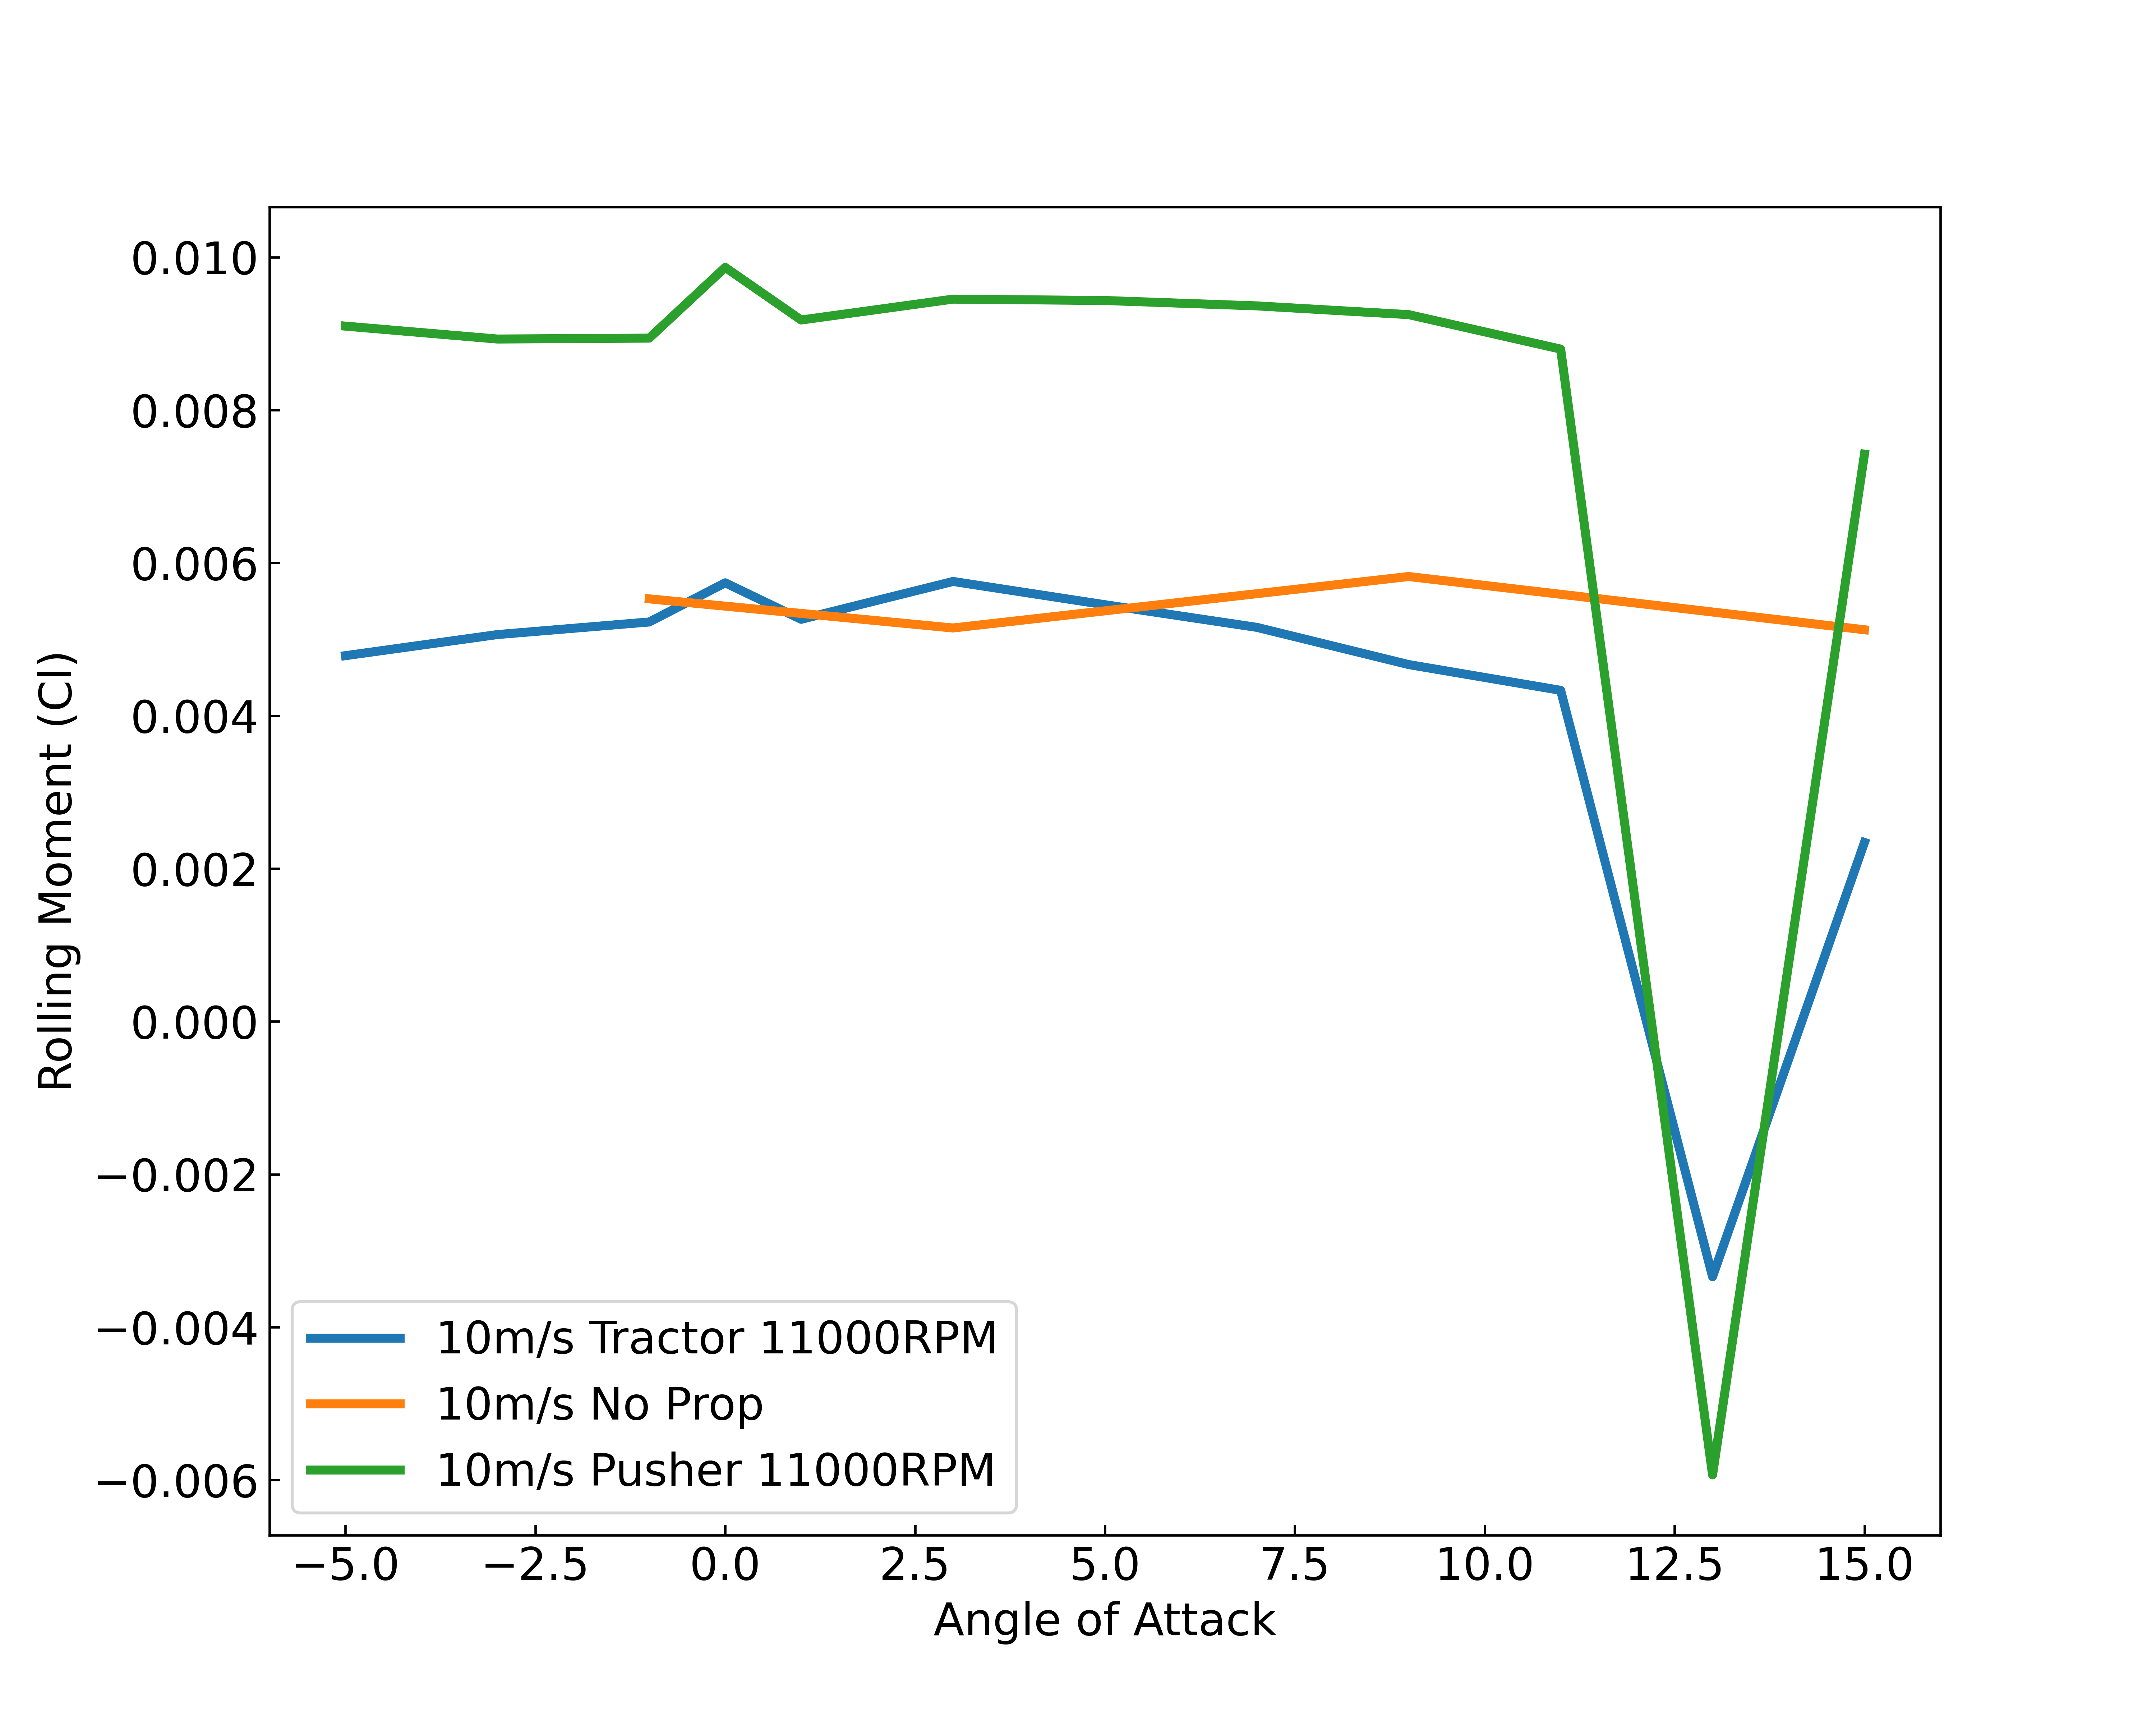
\includegraphics[width=\textwidth]{05_Results/Figs/Cl_roll/10ms_11000RPM_Cl.png}
        \caption{Rolling Moment Coefficient at 10m/s airspeed and 11000RPM motor speed}
        \label{fig:CmCl_10ms_11000}
    \end{subfigure}
    \begin{subfigure}[b]{0.467\textwidth}
        \centering
        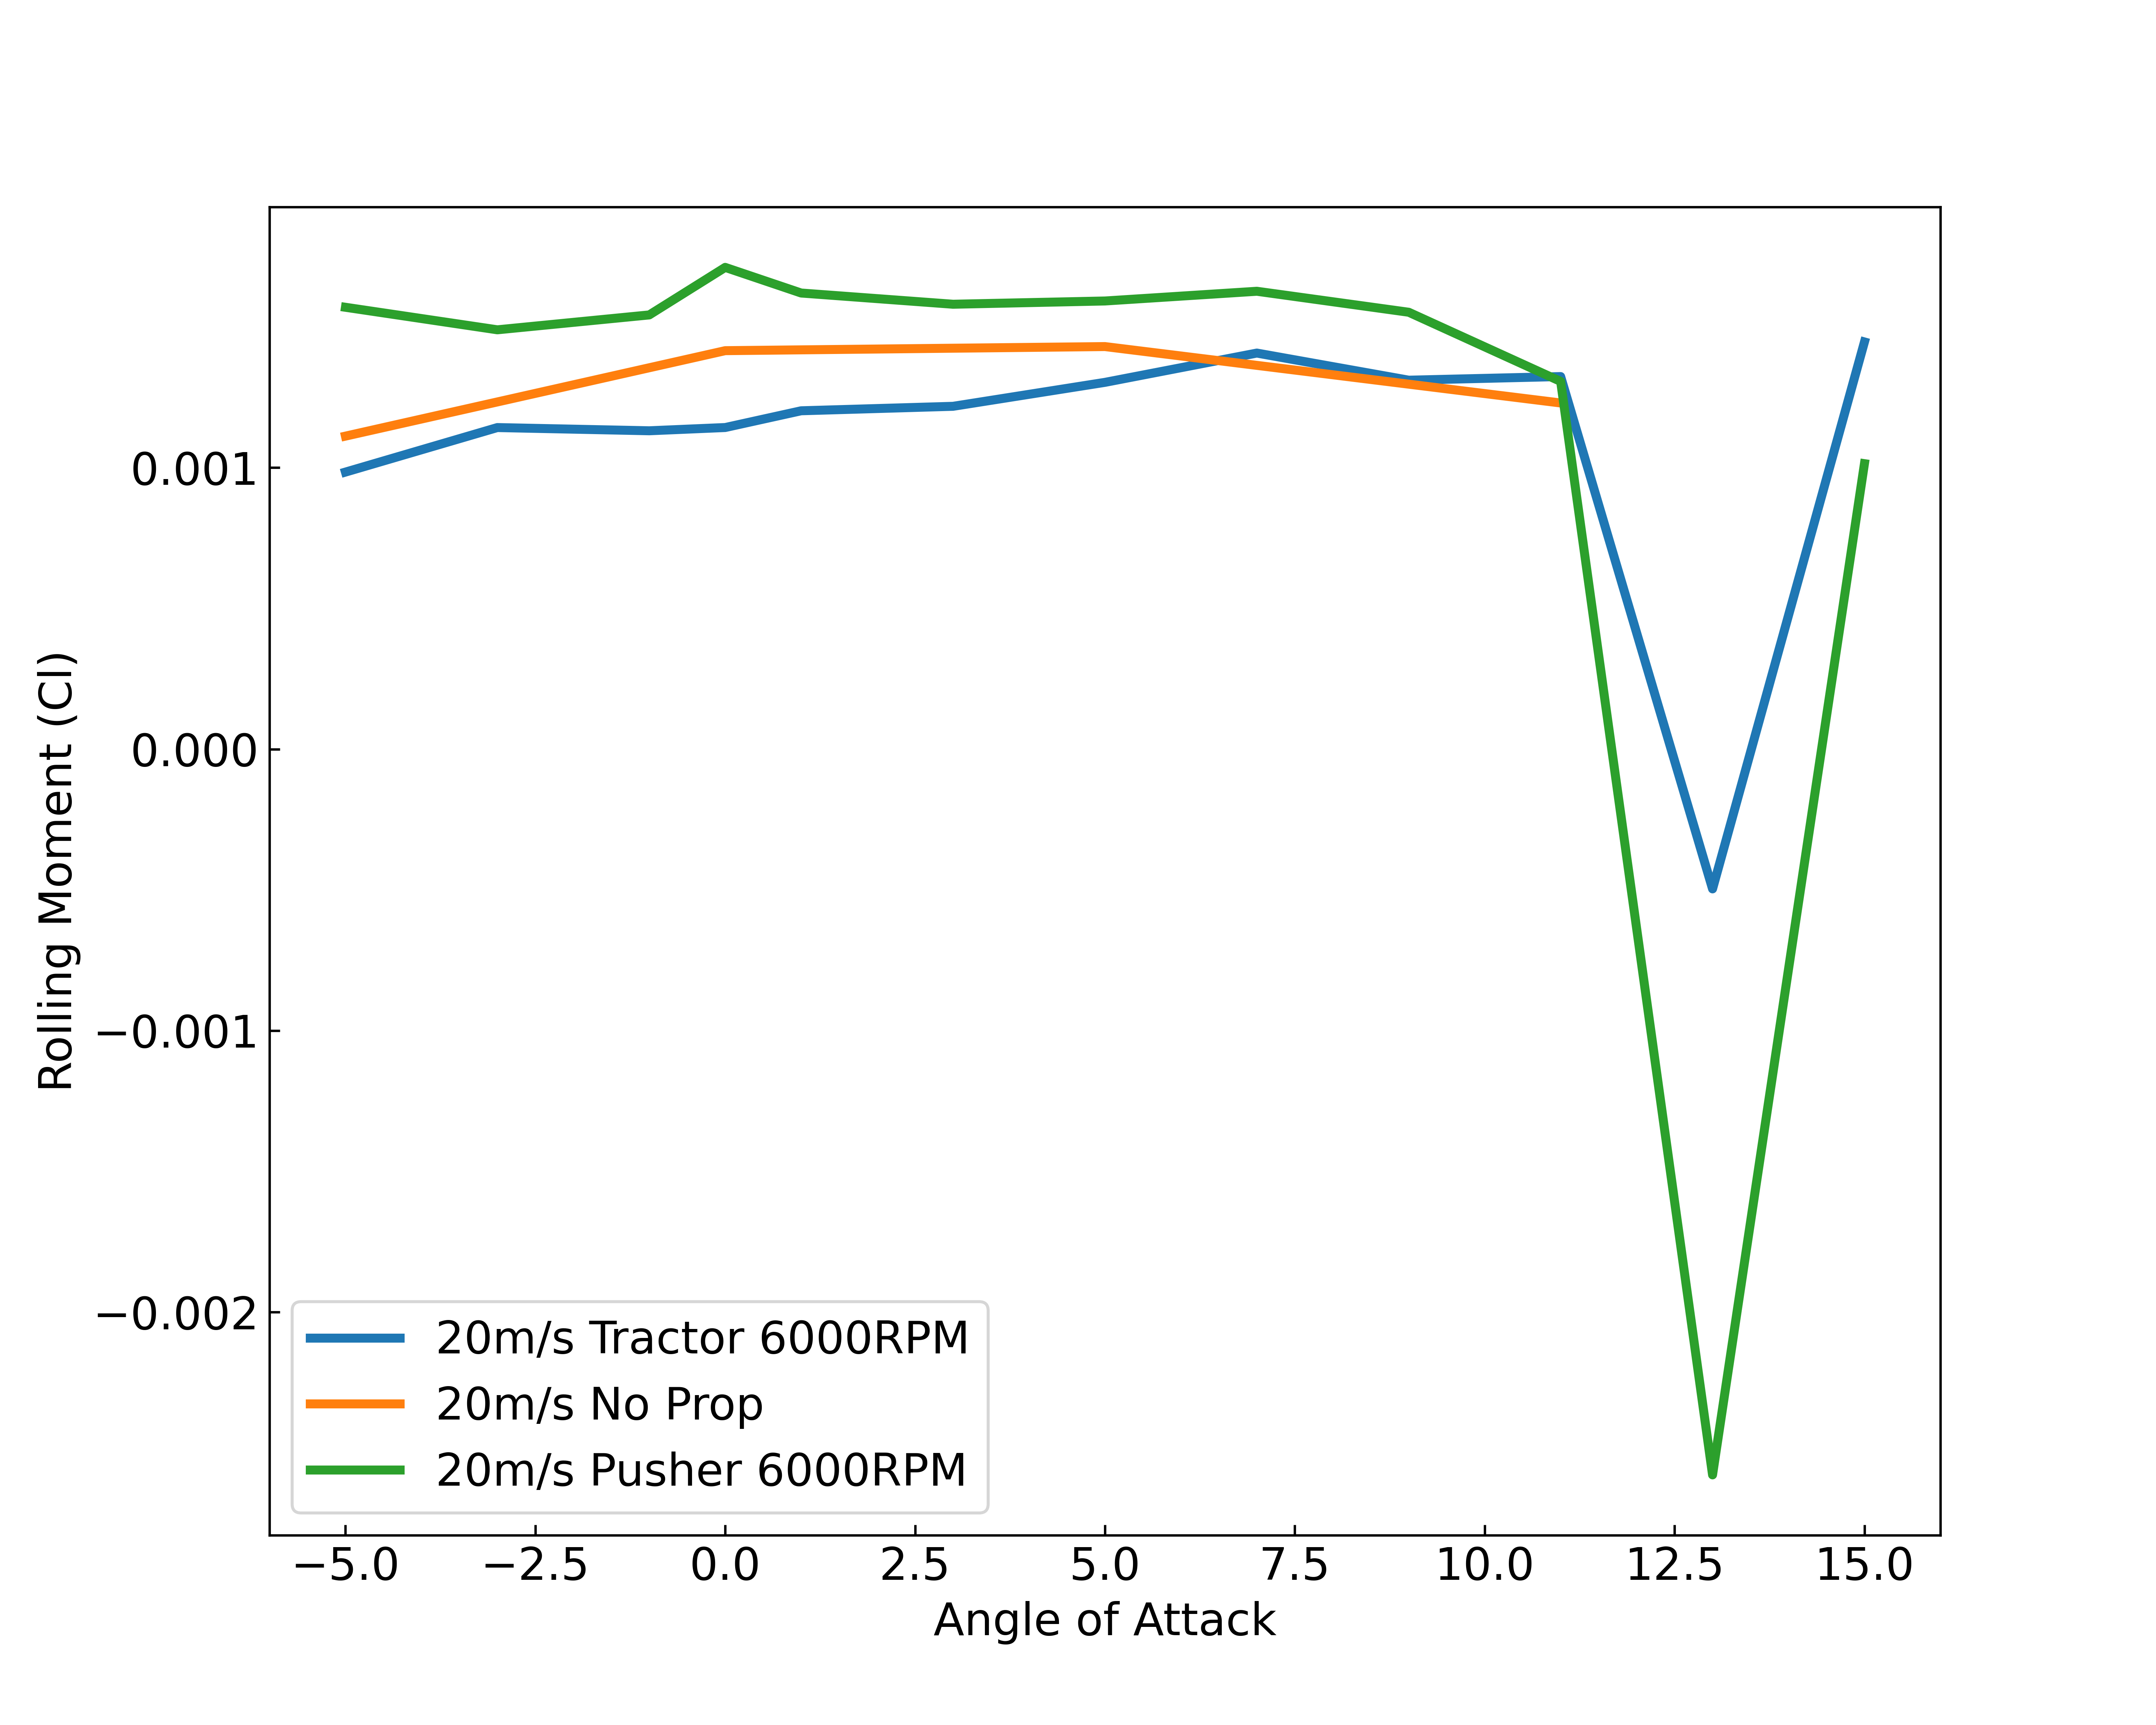
\includegraphics[width=\textwidth]{05_Results/Figs/Cl_roll/20ms_6000RPM_Cl_roll.png}
        \caption{Rolling Moment Coefficient at 20m/s airspeed and 6000RPM motor speed}
        \label{fig:CmCl_20ms_6000}
    \end{subfigure}
    \begin{subfigure}[b]{0.467\textwidth}
        \centering
        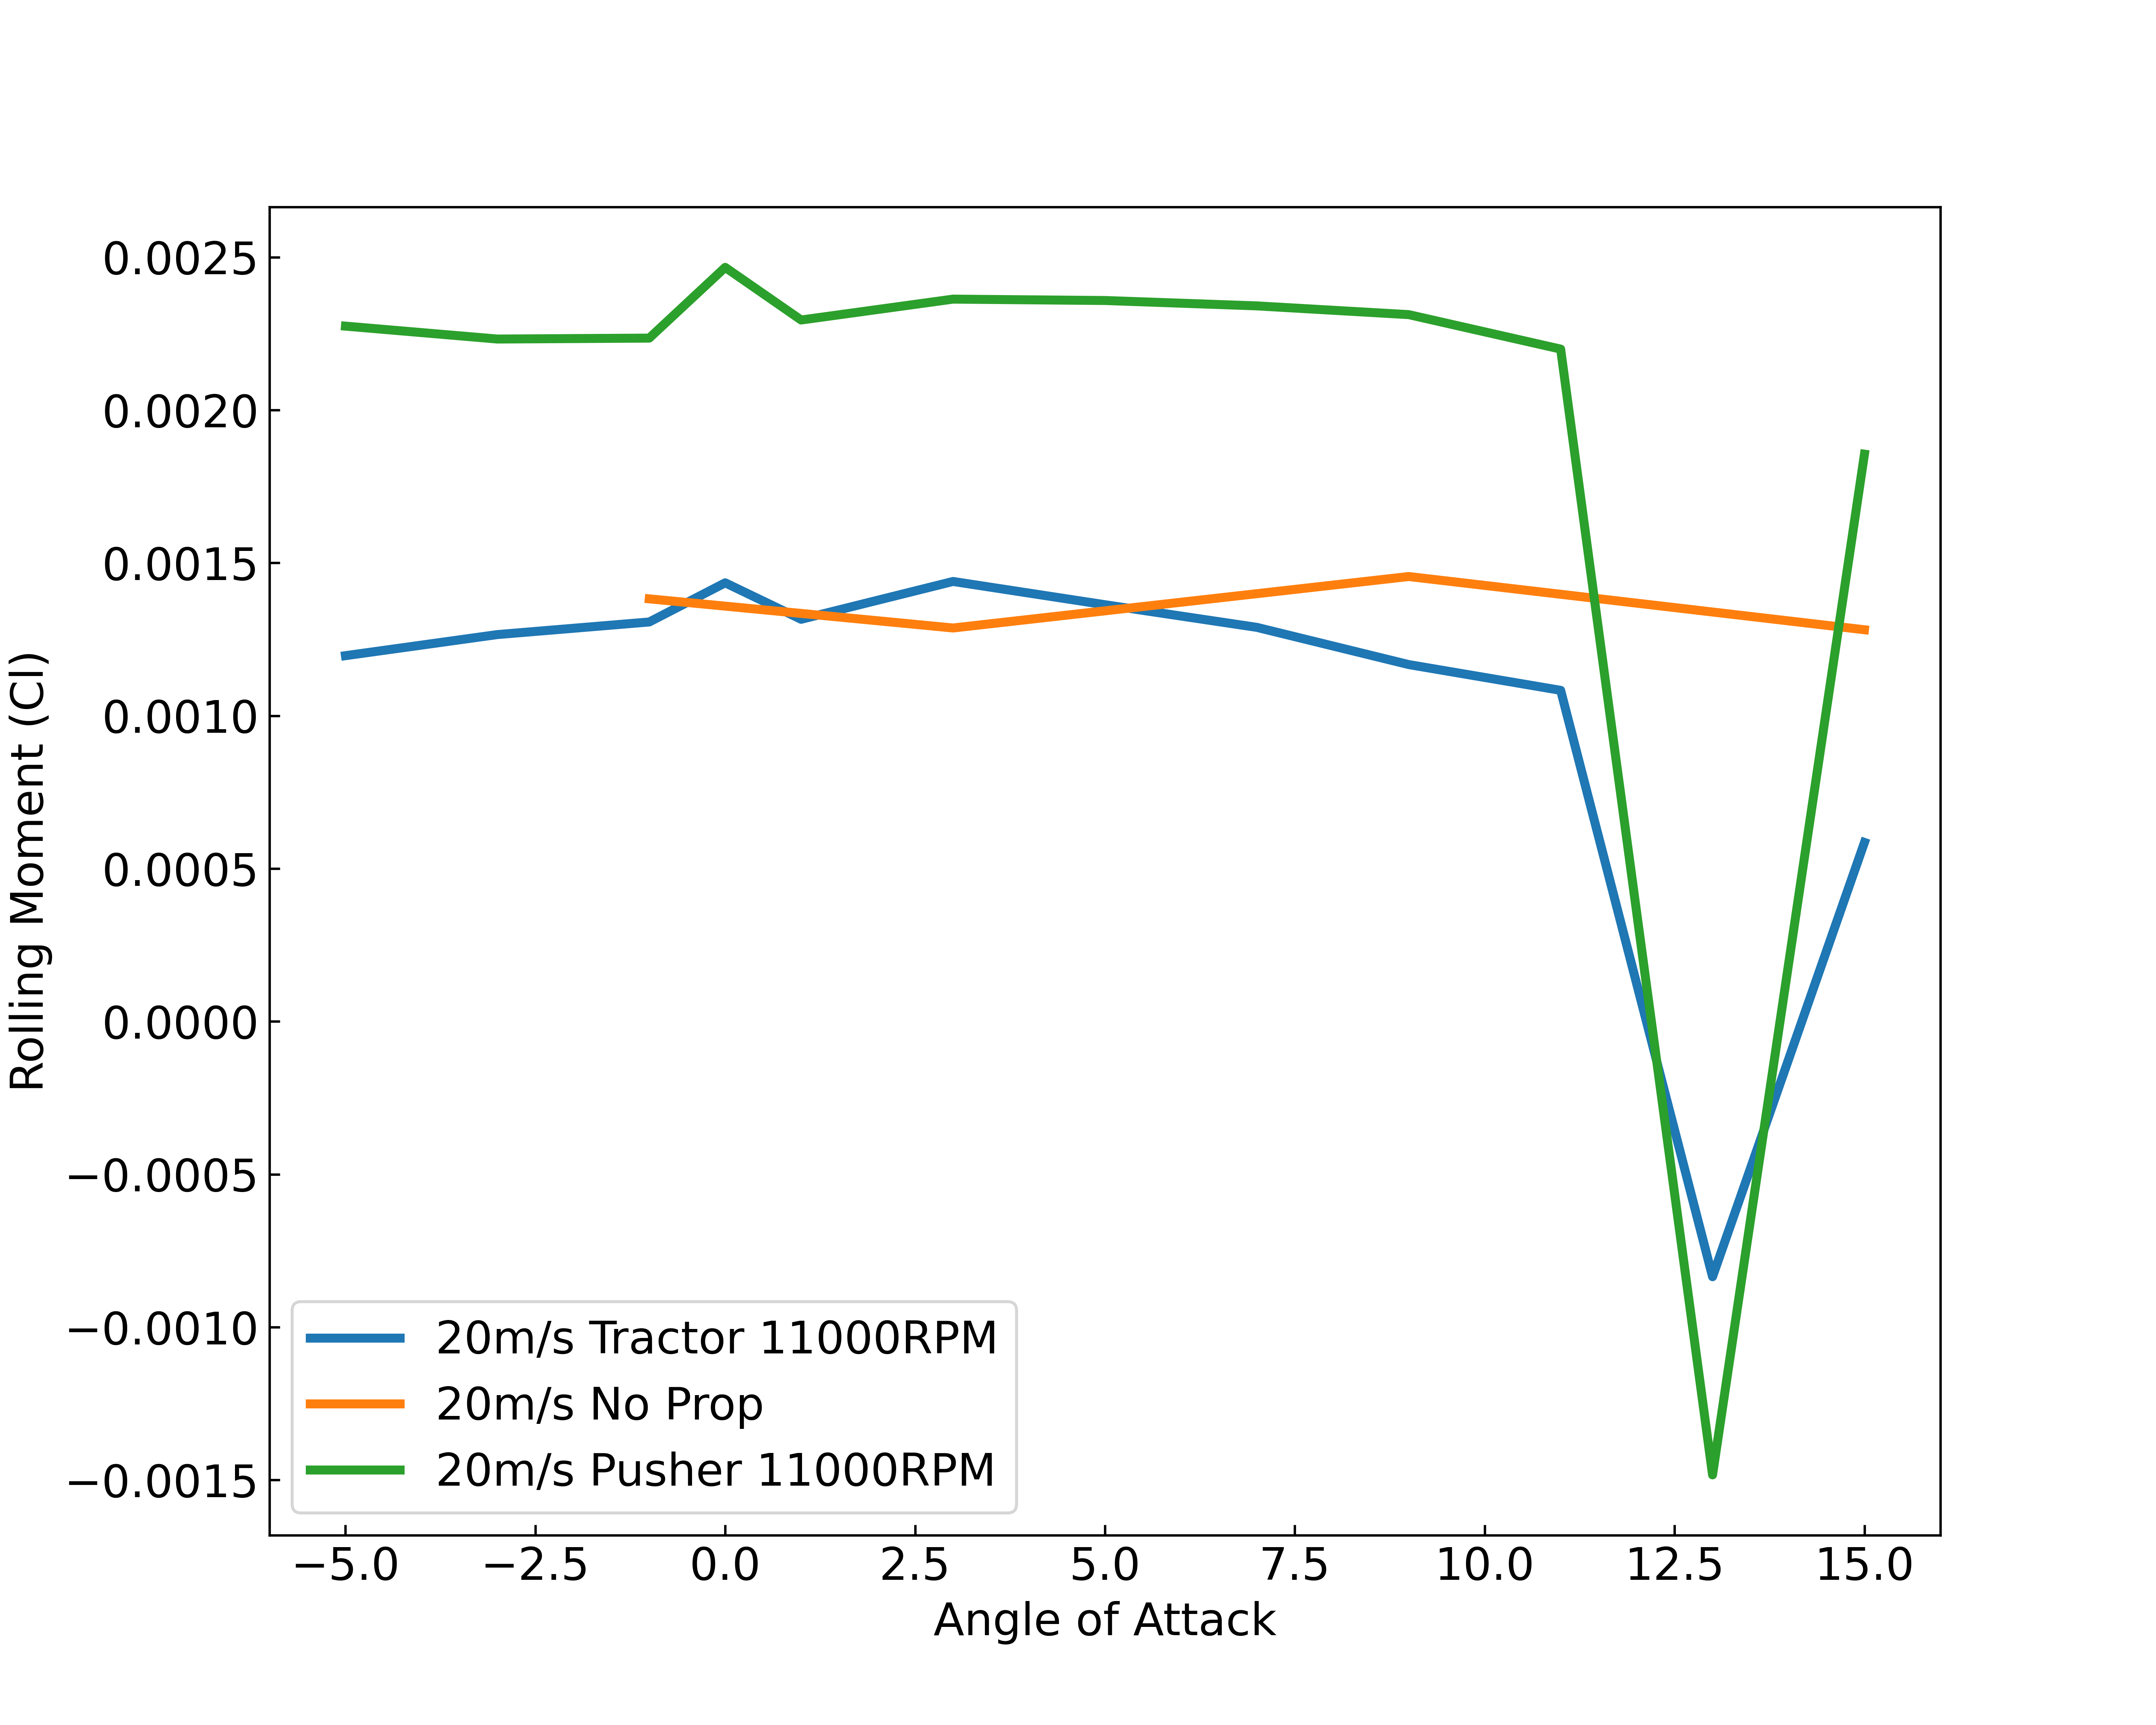
\includegraphics[width=\textwidth]{05_Results/Figs/Cl_roll/20ms_11000RPM_Cl.png}
        \caption{Rolling Moment Coefficient at 20m/s airspeed and 11000RPM motor speed}
        \label{fig:CmCl_20ms_11000}
    \end{subfigure}
\end{figure}


\section{VAP Validation}

\subsection{Wing Validation}


\begin{figure}[H]
     \centering
     \begin{subfigure}[b]{0.45\textwidth}
         \centering
         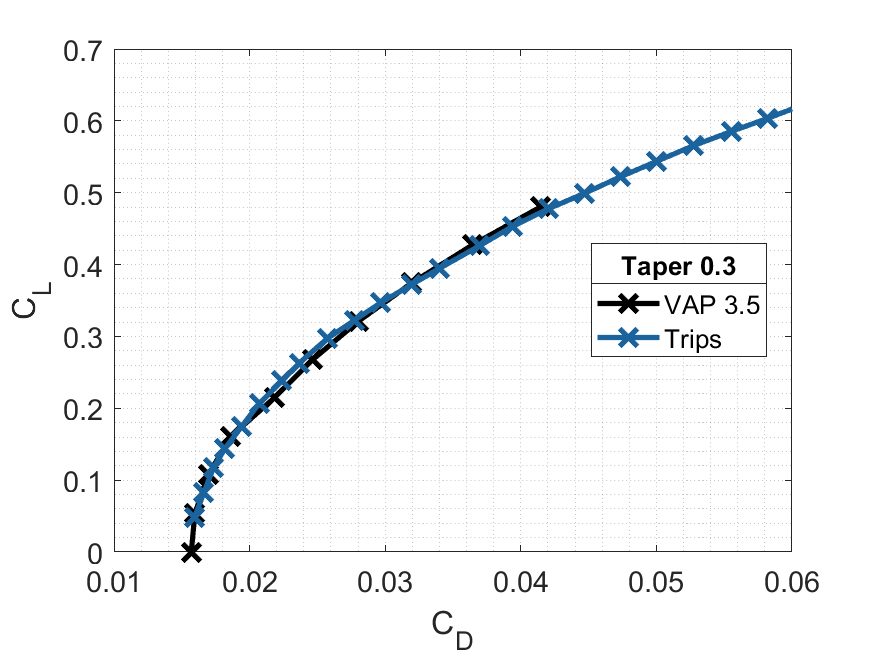
\includegraphics[width=\textwidth]{05_Results/Figs/VAP/genMAV/taper3a.png}

     \end{subfigure}
     \hfill
     \begin{subfigure}[b]{0.45\textwidth}
         \centering
         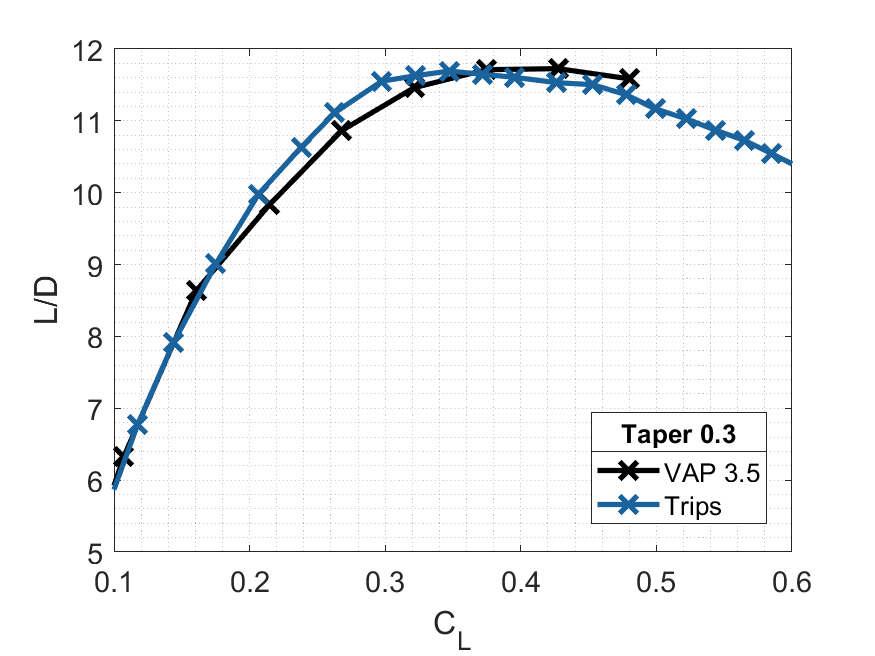
\includegraphics[width=\textwidth]{05_Results/Figs/VAP/genMAV/taper3b.png}
      
     \end{subfigure}
     \hfill

        
\end{figure}


\begin{figure}[H]
     \centering
     \begin{subfigure}[b]{0.45\textwidth}
         \centering
         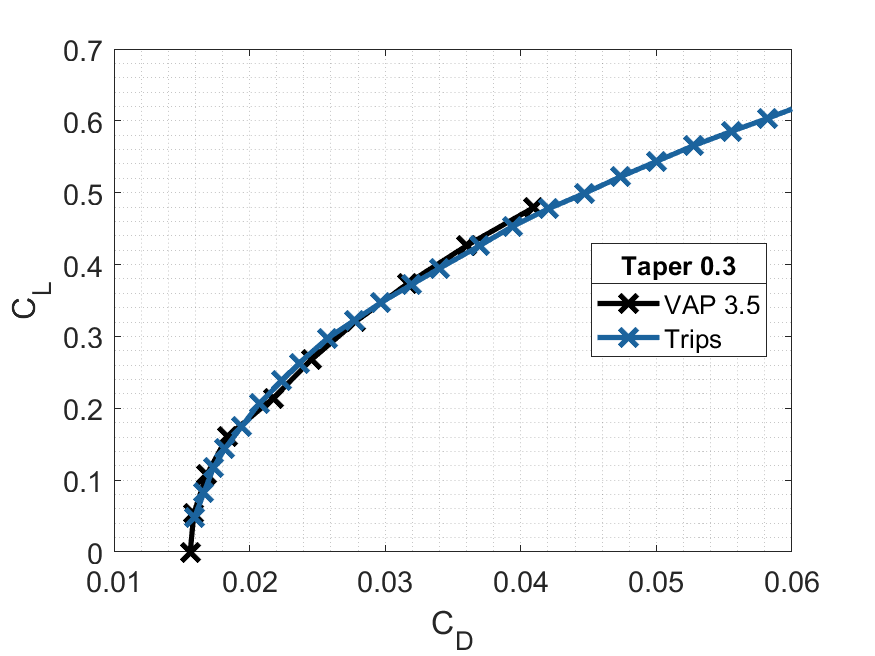
\includegraphics[width=\textwidth]{05_Results/Figs/VAP/genMAV/taper5a.png}

     \end{subfigure}
     \hfill
     \begin{subfigure}[b]{0.45\textwidth}
         \centering
         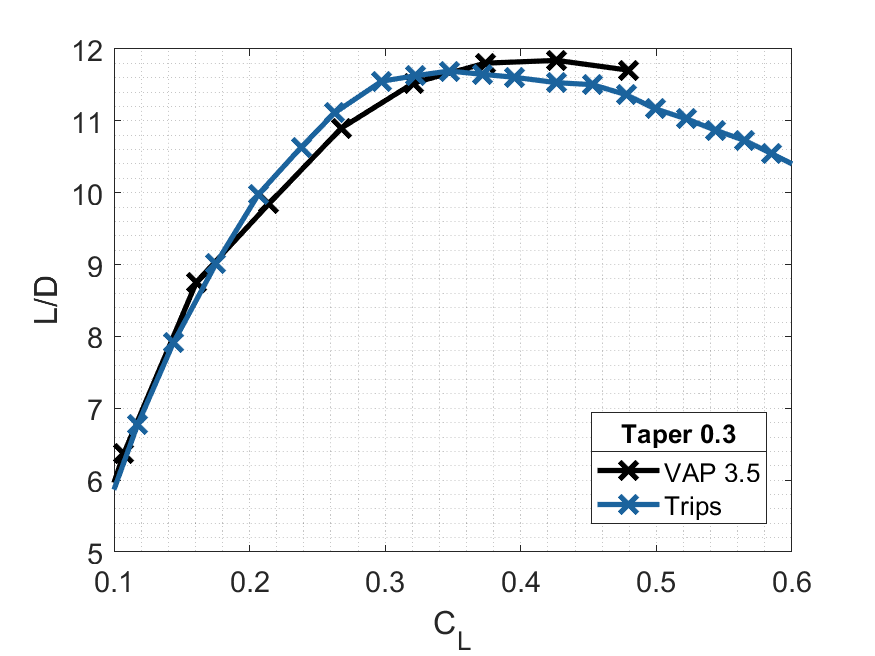
\includegraphics[width=\textwidth]{05_Results/Figs/VAP/genMAV/taper5b.png}
      
     \end{subfigure}
     \hfill

        
\end{figure}


\begin{figure}[H]
     \centering
     \begin{subfigure}[b]{0.45\textwidth}
         \centering
         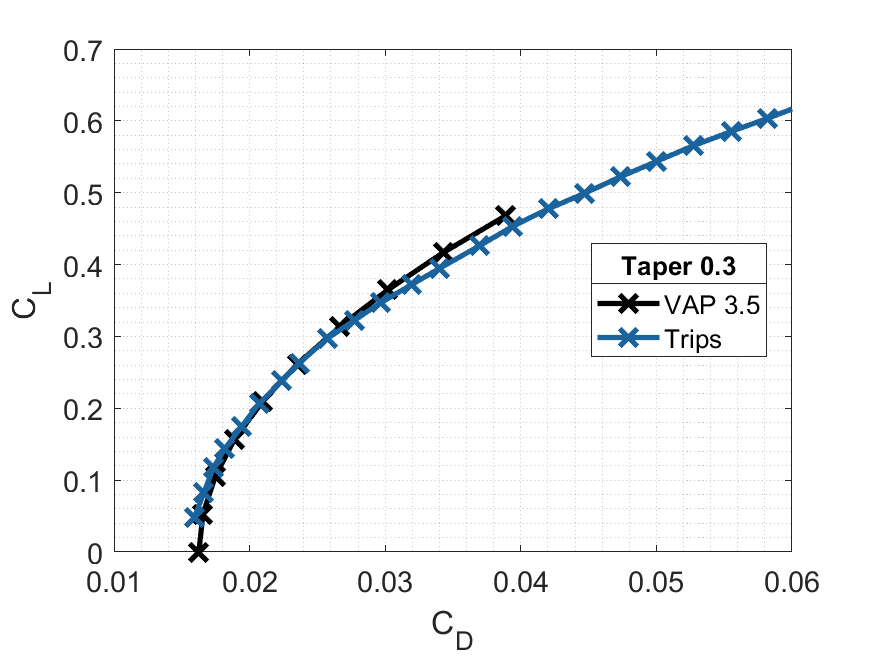
\includegraphics[width=\textwidth]{05_Results/Figs/VAP/genMAV/taper10a.png}

     \end{subfigure}
     \hfill
     \begin{subfigure}[b]{0.45\textwidth}
         \centering
         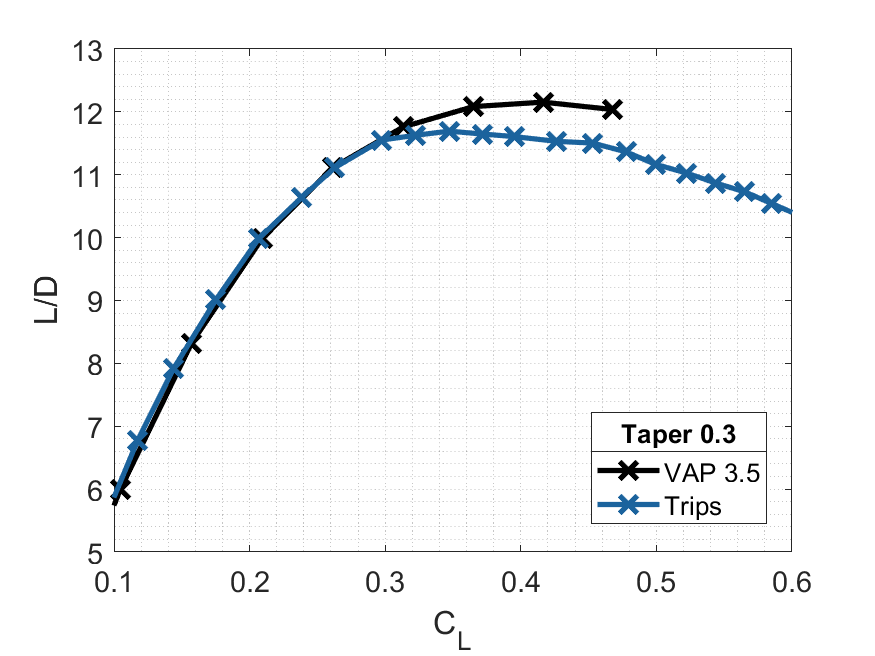
\includegraphics[width=\textwidth]{05_Results/Figs/VAP/genMAV/taper10b.png}
      
     \end{subfigure}
     \hfill

        
\end{figure}

\subsection{Model Validation}

\begin{figure}[H]
    \centering
    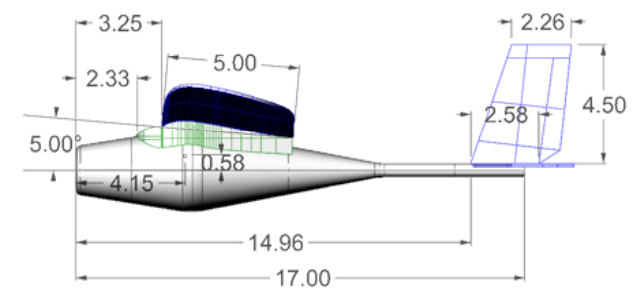
\includegraphics[width=0.5\textwidth]{05_Results/Figs/VAP/genMAV/dimensions.png}
    \label{fig:genMAVDimensions}
\end{figure}

\begin{figure}[H]
         \centering
         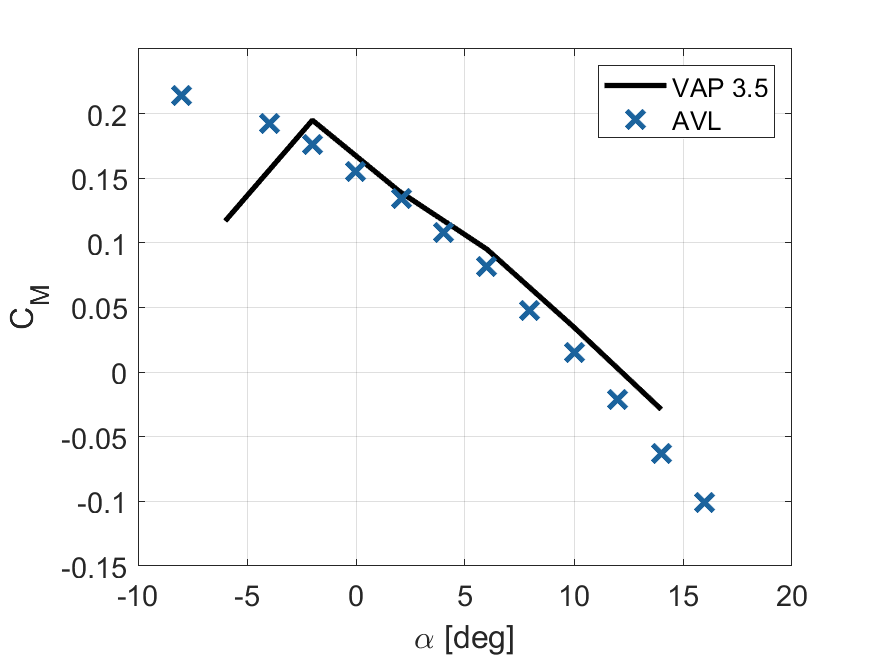
\includegraphics[width=0.5\textwidth]{05_Results/Figs/VAP/genMAV/GenMAVModelValidation1.png}
         \label{fig:genMAV_Cm}
         \caption{}
\end{figure}

\begin{figure}[H]
         \centering
         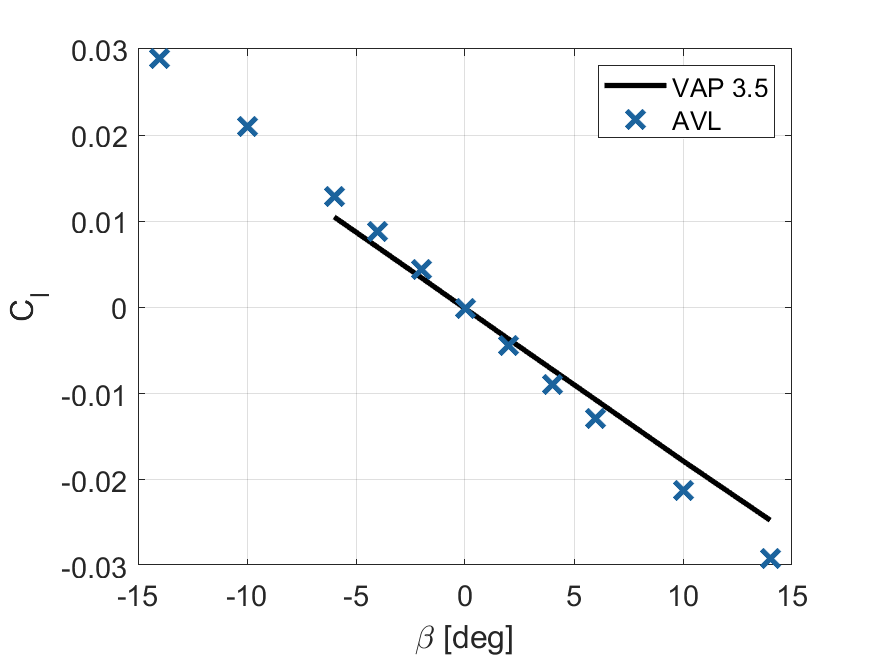
\includegraphics[width=0.5\textwidth]{05_Results/Figs/VAP/genMAV/GenMAVModelValidation2.png}
         \label{fig:genMAV_Cl_roll}
         \caption{}
\end{figure}

\begin{figure}
         \centering
         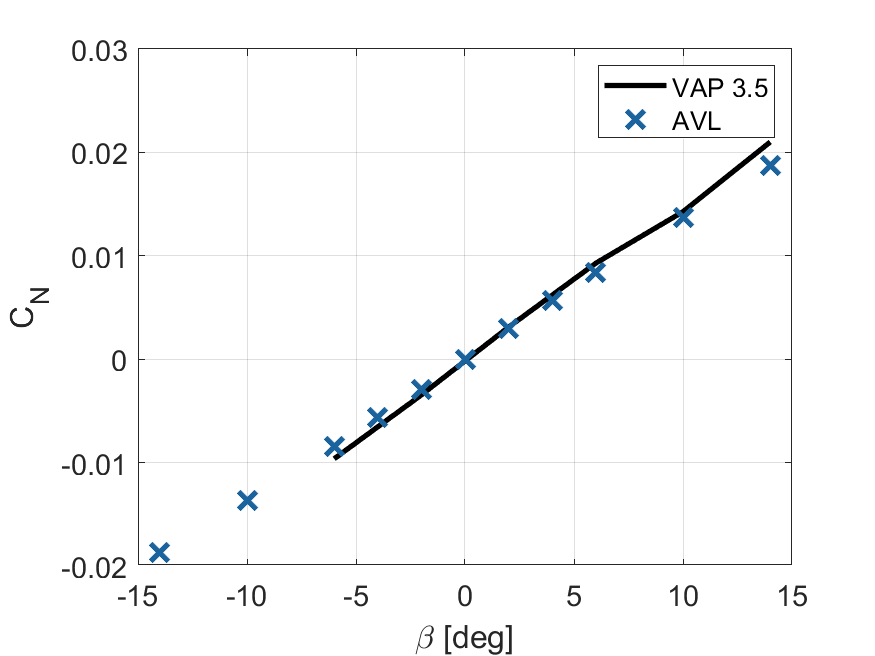
\includegraphics[width=\textwidth]{05_Results/Figs/VAP/genMAV/GenMAVModelValidation3.png}
         \label{fig:genMAV_Cn}
         \caption{}
\end{figure}




\section{Discussion}